\documentclass[a4paper]{report}
\usepackage[main=vietnamese,english]{babel}
\usepackage[utf8]{inputenc}
\usepackage{amsmath}
\usepackage{amsfonts}
\usepackage{amssymb}
\usepackage{graphicx}
\usepackage{xspace}
% \usepackage{caption}
\usepackage[font=small]{caption}
\usepackage{booktabs}
\usepackage[unicode]{hyperref}
\usepackage[left=3cm,right=2cm,top=2.5cm,bottom=3cm]{geometry}
\usepackage{titlesec} 
\usepackage{scrextend}
\usepackage{enumerate}
\usepackage{url}
\usepackage{tikz}
\usepackage{float}
\usepackage{afterpage}
\usepackage{multirow}
\usepackage{sectsty}
\usepackage{tocloft,calc}
\usepackage{listings}
\usepackage{makecell}
% \usepackage[sort&compress]{natbib}
\usetikzlibrary{calc}
\usepackage{algorithm}
\usepackage{subcaption}
\usepackage{biblatex}
% \usepackage[perpage]{footmisc}
\usepackage[flushleft]{threeparttable}
% \usepackage{subcaption}
\usepackage{perpage} %the perpage package
\addbibresource{references.bib}
\MakePerPage{footnote} %the perpage package command
% \usepackage[ruled,vlined]{algorithm2e}
\PassOptionsToPackage{table}{xcolor}

\def\changemargin#1#2{\list{}{\rightmargin#2\leftmargin#1}\item[]}
\let\endchangemargin=\endlist 

\changefontsizes{13pt}
% \bibliographystyle{unsrt}

\makeatletter
\def\l@figure{\@dottedtocline{1}{1em}{2.2em}}
\def\l@table{\@dottedtocline{1}{1em}{2.2em}}
\renewcommand*{\ALG@name}{Thuật toán}
\makeatother

\sectionfont{\fontsize{15}{15}\selectfont}
\subsectionfont{\fontsize{13}{15}\selectfont}

\titleformat{\chapter}[display]   
{\normalfont\LARGE\bfseries}{\chaptertitlename\ \thechapter}{0pt}{\LARGE}
\titlespacing*{\chapter}{0cm}{-\topskip}{0pt}[0pt]

\renewcommand{\baselinestretch}{1.3}
\newcommand{\nl}{\\[0.6em]}
%\renewcommand{\cftsecpresnum}{Chương\space}
\renewcommand{\cftchappresnum}{Chương }
\AtBeginDocument{\addtolength\cftchapnumwidth{\widthof{\bfseries Chương }}}
\setlength{\parskip}{0.6em}
\setlength{\parindent}{1.5em}
%
\title{Hệ thống kết nối người yêu thích du lịch, lên kế hoạch và chia sẻ trải nghiệm}	%% title
\author{Nguyễn Nhật Minh}			%% author's name

%
\newcommand{\argmax}{\arg\!\max}
\newcommand{\tool}{\textsc{DeFP}\xspace}
\newcommand{\toolLong}{\textbf{De}tect \textbf{F}alse \textbf{P}ositive\xspace}

\definecolor{dkgreen}{rgb}{0,0.6,0}
\definecolor{gray}{rgb}{0.5,0.5,0.5}
\definecolor{mauve}{rgb}{0.58,0,0.82}
\definecolor{gray}{rgb}{0.4,0.4,0.4}
\definecolor{darkblue}{rgb}{0.0,0.0,0.6}
\definecolor{lightblue}{rgb}{0.0,0.0,0.9}
\definecolor{cyan}{rgb}{0.0,0.6,0.6}
\definecolor{darkred}{rgb}{0.6,0.0,0.0}
\definecolor{bg_gray}{RGB}{242, 242, 235}

\renewcommand{\lstlistingname}{Hình}
\newcommand{\cev}[1]{\reflectbox{\ensuremath{\vec{\reflectbox{\ensuremath{#1}}}}}}

\lstset{
  basicstyle=\ttfamily\footnotesize,
  columns=fullflexible,
  showstringspaces=false,
  numbers=left,                   % where to put the line-numbers
  numberstyle=\small\color{gray},  % the style that is used for the line-numbers
  stepnumber=1,
  numbersep=5pt,                  % how far the line-numbers are from the code
  backgroundcolor=\color{bg_gray},      % choose the background color. You must add \usepackage{color}
  showspaces=false,               % show spaces adding particular underscores
  showstringspaces=false,         % underline spaces within strings
  showtabs=false,                 % show tabs within strings adding particular underscores
  frame=none,                   % adds a frame around the code
  rulecolor=\color{black},        % if not set, the frame-color may be changed on line-breaks within not-black text (e.g. commens (green here))
  tabsize=2,                      % sets default tabsize to 2 spaces
  captionpos=b,                   % sets the caption-position to bottom
  breaklines=true,                % sets automatic line breaking
  breakatwhitespace=false,        % sets if automatic breaks should only happen at whitespace
  title=\lstname,                   % show the filename of files included with \lstinputlisting;
                                  % also try caption instead of title  
  commentstyle=\color{gray}\upshape
}


\lstdefinelanguage{XML}
{
  morestring=[s][\color{mauve}]{"}{"},
  morestring=[s][\color{black}]{>}{<},
  morecomment=[s]{<?}{?>},
  morecomment=[s][\color{dkgreen}]{<!--}{-->},
  stringstyle=\color{black},
  identifierstyle=\color{lightblue},
  keywordstyle=\color{red},
  morekeywords={xmlns,xsi,noNamespaceSchemaLocation,type,id,x,y,source,target,version,tool,transRef,roleRef,objective,eventually}% list your attributes here
}

\definecolor{codegreen}{rgb}{0,0.6,0}
\definecolor{codegray}{rgb}{0.5,0.5,0.5}
\definecolor{codepurple}{rgb}{0.58,0,0.82}
\definecolor{backcolour}{rgb}{0.95,0.95,0.92}

\begin{document}
% Cover Vietnamese 1

% Cover Vietnamese 1

% Cover english
\pagenumbering{gobble}
\begin{center}
	\begin{tikzpicture}[overlay,remember picture]
	    \draw [line width=3pt,rounded corners=0pt,
	        ]
	        ($ (current page.north west) + (25mm,-25mm) $)
	        rectangle
	        ($ (current page.south east) + (-15mm,25mm) $);
	    \draw [line width=1pt,rounded corners=0pt]
	        ($ (current page.north west) + (26.5mm,-26.5mm) $)
	        rectangle
	        ($ (current page.south east) + (-16.5mm,26.5mm) $);
	\end{tikzpicture}
	\\[1mm]
	%%12pt
	\textbf{ĐẠI HỌC QUỐC GIA HÀ NỘI\\TRƯỜNG ĐẠI HỌC CÔNG NGHỆ}\\[1cm]
	
\includegraphics[width=0.2\linewidth]{figures/uet}\\[0.3cm]
	\Large{\textbf{Nguyễn Nhật Minh}}
	\\[2cm]
	
	\large{\textbf{HỆ THỐNG KẾT NỐI NGƯỜI YÊU THÍCH DU LỊCH, LÊN KẾ HOẠCH VÀ CHIA SẺ CÁC TRẢI NGHIỆM}}
	\\[2.6cm]
	\normalsize{\textbf{KHOÁ LUẬN TỐT NGHIỆP ĐẠI HỌC
		\\[2mm]
	Ngành: Công nghệ thông tin}}

	\vfill
	\textbf{HÀ NỘI - 2025}
	\vspace{10mm}
\end{center}

\begin{center}
	
	\begin{tikzpicture}[overlay,remember picture]
	\draw [line width=3pt,rounded corners=0pt,
	]
	($ (current page.north west) + (25mm,-25mm) $)
	rectangle
	($ (current page.south east) + (-15mm,25mm) $);
	\draw [line width=1pt,rounded corners=0pt]
	($ (current page.north west) + (26.5mm,-26.5mm) $)
	rectangle
	($ (current page.south east) + (-16.5mm,26.5mm) $);
	\end{tikzpicture}
	\\[1mm]
	\textbf{ĐẠI HỌC QUỐC GIA HÀ NỘI\\TRƯỜNG ĐẠI HỌC CÔNG NGHỆ}
	\\[1cm]
	
\includegraphics[width=0.2\linewidth]{figures/uet}
	\\[0.3cm]
	\Large{\textbf{Nguyễn Nhật Minh}}
	\\[2cm]
	
	\large{\textbf{HỆ THỐNG KẾT NỐI NGƯỜI YÊU THÍCH DU LỊCH, LÊN KẾ HOẠCH VÀ CHIA SẺ CÁC TRẢI NGHIỆM}}
	\\[2.6cm]
	\normalsize{\textbf{KHOÁ LUẬN TỐT NGHIỆP ĐẠI HỌC
		\\[2mm]
	Ngành: Công nghệ thông tin}}
\end{center}
\vspace{16mm}
\hspace*{12mm}\textbf{ Cán bộ hướng dẫn: TS. Lê Khánh Trình}\\[0.2cm]
\hspace*{12mm}\textbf{ Cán bộ đồng hướng dẫn: TS. Đặng Trần Bình}
\vfill
\begin{center}
	\textbf{HÀ NỘI - 2025}
	\vspace{10mm}
\end{center}


% \begin{center}
	
% 	\begin{tikzpicture}[overlay,remember picture]
% 	\draw [line width=3pt,rounded corners=0pt,
% 	]
% 	($ (current page.north west) + (25mm,-25mm) $)
% 	rectangle
% 	($ (current page.south east) + (-15mm,25mm) $);
% 	\draw [line width=1pt,rounded corners=0pt]
% 	($ (current page.north west) + (26.5mm,-26.5mm) $)
% 	rectangle
% 	($ (current page.south east) + (-16.5mm,26.5mm) $);
% 	\end{tikzpicture}
% 	\\[1mm]
% 	\textbf{ VIETNAM NATIONAL UNIVERSITY, HANOI\\UNIVERSITY OF ENGINEERING AND TECHNOLOGY}
% 	\\[1cm]
% 	
\includegraphics[width=0.2\linewidth]{figures/uet}
% 	\\[0.3cm]
% 	\textbf{Nguyen Van A}
% 	\\[2cm]
	
% 	\textbf{THESIS TITLE}
% 	\\[2.6cm]
% 	\textbf{BACHELOR'S THESIS
% 		\\[2mm]
% 		Major: Information technology}
% \end{center}
% \vspace{16mm}
% \hspace*{12mm}\textbf{ Supervisor: Dr. ...}\\[0.8cm]
% \hspace*{12mm}\textbf{ Co-Supervisor: Dr. ...}
% \vfill
% \begin{center}
% 	\textbf{HANOI - 2022}
% 	\vspace{4mm}
% \end{center}

\newpage\cleardoublepage

% Acknowledgement
\begin{center}
\textbf{\large{Lời cảm ơn}	}
\end{center}
\addcontentsline{toc}{chapter}{Lời cảm ơn}
 Lời đầu tiên em xin chân thành cảm ơn tập thể các Giảng viên Trường Đại học Công
 nghệ nói chung và Khoa Công Nghệ Thông Tin nói riêng đã tận tình giảng dạy
 truyền đạt cho em kiến thức, kinh nghiệm quý giá trong suốt 4 năm học vừa
 qua.
 \nl
 \indent Tiếp theo em xin bày tỏ lòng biết ơn sâu sắc tới Thầy giáo, TS. Lê Khánh
 Trình, Khoa Công nghệ Thông tin– Trường Đại học Công nghệ- ĐHQGHN. Trong
 quá trình từ khi được Thầy giảng dạy hướng dẫn, Thầy vẫn luôn ủng hộ và động
 viên em và đưa ra hướng đi phù hợp với khả năng của mình. Nhờ sự quan tâm chỉ bảo và những ý kiến đóng góp quý báu
 của Thầy, em mới có thể tiếp tục và hoàn thiện luận văn này.\nl
 \indent Em cũng xin cảm ơn các bạn sinh viên đã luôn sẵn sàng chia sẻ, hỗ trợ và động viên em trong quá trình nghiên cứu và thực hiện đồ án. Những cuộc thảo luận, góp ý từ mọi người đã giúp em có nhiều góc nhìn mới và cải thiện chất lượng của luận văn này.\nl
 \indent Cuối cùng em xin chân thành cảm ơn gia đình, người thân đã hết lòng giúp
 đỡ, hỗ trợ về vật chất lẫn tinh thần giúp em yên tâm học tập và nghiên cứu trong
 suốt quá trình học tập và thực hiện luận văn.

 \indent Mặc dù đã cố gắng hết sức để hoàn thành đồ án một cách hoàn thiện nhất, nhưng chắc chắn vẫn không thể tránh khỏi những thiếu sót. Em rất mong nhận được sự góp ý từ thầy cô và các bạn để có thể tiếp tục hoàn thiện và phát triển hơn trong tương lai.\newpage\cleardoublepage
% Assurance
\setcounter{page}{1}
\pagenumbering{roman}
\begin{center}
\textbf{\large{Lời cam đoan}	}
\end{center}
\addcontentsline{toc}{chapter}{Lời cam đoan}
Em là Nguyễn Nhật Minh, sinh viên lớp QH-2021-J khóa K66 theo học ngành Công nghệ thông tin tại trường Đại học Công Nghệ - Đại học Quốc gia Hà Nội. Em xin cam đoan khoá luận ``Hệ thống kết nối người yêu thích du lịch tích hợp AI tổng hợp lịch trình'' là công trình nghiên cứu do bản thân em thực hiện. Các nội dung nghiên cứu, kết quả trong khoá luận là xác thực.

Các thông tin sử dụng trong khoá luận là có cơ sở và không có nội dung nào sao chép từ các tài liệu mà không ghi rõ trích dẫn tham khảo. Tôi xin chịu trách nhiệm về lời cam đoan này.

\begin{flushright}
Hà Nội, ngày 30 tháng 3 năm 2025
\end{flushright}

\begin{changemargin}{12cm}{2cm}
Sinh viên
\\[2cm]
\end{changemargin}

\begin{changemargin}{11cm}{1cm}
Nguyễn Nhật Minh
\end{changemargin}\newpage\cleardoublepage
% \begin{center}
% \textbf{\large{Tóm tắt}	}
% \end{center}
% \addcontentsline{toc}{chapter}{Tóm tắt}
% Khóa luận tập trung xây dựng một ứng dụng di động \textbf{VieVu} hỗ trợ lập kế hoạch du lịch,  
% tìm kiếm bạn đồng hành và quản lý lịch trình chuyến đi một cách hiệu quả và dành riêng cho du lịch trong Việt Nam. 
% Ứng dụng cung cấp giao diện thân thiện, cho phép người dùng tạo, 
% chỉnh sửa kế hoạch du lịch cá nhân hoặc nhóm và chia sẻ, đăng tải chuyến đi đó cho. 
% Một trong những tính năng cốt lõi của hệ thống là khả năng 
% tự động trích xuất và tổng hợp thông tin lịch trình từ hội 
% thoại nhóm, giúp người dùng dễ dàng theo dõi các mốc thời gian, 
% địa điểm và sự kiện quan trọng trong chuyến đi.

% Bên cạnh đó, hệ thống ứng dụng AI và NLP để phân loại nội dung tin nhắn, nhận diện các hoạt động du lịch. Ngoài ra, ứng dụng còn tích hợp hệ thống gợi ý địa điểm dựa trên nội dung và đánh giá của người dùng khác, giúp cá nhân hóa trải nghiệm du lịch dựa trên sở thích, ngân sách và loại hình du lịch ưa thích của người dùng.

% Khóa luận không chỉ tập trung vào việc xây dựng nền tảng kỹ thuật vững chắc mà còn đảm bảo tính tiện ích và tối ưu hóa trải nghiệm người dùng, hướng đến một giải pháp hỗ trợ du lịch thông minh, hiệu quả và linh hoạt.

% \vspace{0.5cm}
% \noindent \textbf{Từ khóa}: Ứng dụng du lịch, VieVu, Tổng hợp lịch trình, Gợi ý địa điểm, Lập kế hoạch chuyến đi.


% \begin{flushright}
% Hà Nội, ngày 30 tháng 3 năm 2025
% \end{flushright}

% \begin{changemargin}{12cm}{2cm}
% Sinh viên
% \\[2cm]
% \end{changemargin}

% \begin{changemargin}{11cm}{1cm}
% Nguyễn Nhật Minh
% \end{changemargin}

\begin{center}
\textbf{\large{Tóm tắt}}
\end{center}
\addcontentsline{toc}{chapter}{Tóm tắt}
Khóa luận tập trung xây dựng ứng dụng di động \textbf{VieVu}, nền tảng hỗ trợ lập kế hoạch chuyến đi, tìm kiếm bạn đồng hành và quản lý lịch trình du lịch một cách thông minh. Ứng dụng được thiết kế dành riêng cho du lịch tại Việt Nam, giúp người dùng dễ dàng khám phá các chuyến đi, kết nối với cộng đồng du lịch và tham gia vào hành trình phù hợp.  
VieVu cho phép người dùng tạo, quản lý và đăng bài về chuyến đi du lịch trên news feed, nơi những người quan tâm có thể tìm kiếm, tương tác và tham gia. Bên cạnh đó, hệ thống tích hợp AI để tự động phân loại tin nhắn, trích xuất thông tin địa điểm và tổng hợp lịch trình từ hội thoại nhóm, giúp tạo lịch trình từ những ý kiến thảo luận của các thành viên.  
Ngoài ra, VieVu cũng gợi ý địa điểm dựa trên nội dung và đánh giá từ cộng đồng, cá nhân hóa trải nghiệm du lịch theo sở thích, ngân sách và loại hình du lịch.  
Khóa luận không chỉ tập trung vào việc xây dựng một nền tảng kỹ thuật vững chắc mà còn hướng đến trải nghiệm người dùng mượt mà, giúp việc lập kế hoạch du lịch trở nên dễ dàng, tiện lợi và kết nối hơn bao giờ hết.  
    
\vspace{0.5cm}
\noindent \textbf{Từ khóa}: Ứng dụng du lịch, VieVu, Zeroshot Classification, AI,  Hybrid Recommendation, Chia sẻ vị trí, Tổng hợp lịch trình.
    \newpage\cleardoublepage
% % Abstract Vietnamese
% \begin{center}
\textbf{\large{Tóm tắt}	}
\end{center}

\addcontentsline{toc}{chapter}{Tóm tắt}

\begin{small}



\vspace*{1cm}
\textbf{Từ khóa}: 

\end{small}\newpage\cleardoublepage
% % Abstract English
% \begin{center}
\textbf{\large{Abstract}	}
\end{center}

\addcontentsline{toc}{chapter}{Abstract}
\begin{small}



\vspace*{1cm}
\textbf{Keywords}: 
\end{small}\newpage\cleardoublepage
\addcontentsline{toc}{chapter}{Mục lục}
\tableofcontents\newpage\cleardoublepage
% %

% \newpage
% \addcontentsline{toc}{chapter}{\listfigurename}
% \listoffigures\cleardoublepage

% \newpage
% \addcontentsline{toc}{chapter}{\listtablename}
% \listoftables

% \newpage
% \chapter*{Danh mục các từ viết tắt}
\addcontentsline{toc}{chapter}{Danh mục các từ viết tắt}

%\begin{tabular}{|l|l|l|l|}
\begin{tabular}{|m{0.8cm}|m{2.2 cm}|m{5.2cm}|m{6.2cm}|}
    \hline
\thead{\textbf{STT}} & \thead{\textbf{Từ viết tắt}} & \thead{\textbf{Cụm từ đầy đủ}} & \thead{\textbf{Cụm từ tiếng Việt}} \\
                    \hline
1 & AI & Artificial Intelligence & Trí tuệ nhân tạo \\ \hline
2 & NLP & Natural Language Processing & Xử lý ngôn ngữ tự nhiên \\ \hline
3 & NER & Named Entity Recognition & Nhận dạng thực thể có tên \\ \hline
4 & ZSC & Zero-Shot Classification & Phân loại không cần mẫu (Zero-Shot) \\ \hline
5 & LLM & Large Language Model & Mô hình ngôn ngữ lớn \\ \hline
6 & API & Application Programming Interface & Giao diện lập trình ứng dụng \\ \hline
7 & BaaS & Backend as a Service & Backend dưới dạng dịch vụ \\ \hline
8 & UI & User Interface & Giao diện người dùng \\ \hline
9 & SQL & Structured Query Language & Ngôn ngữ truy vấn có cấu trúc \\ \hline
10 & JWT & JSON Web Token & Mã thông báo web JSON \\ \hline

\end{tabular}\newpage\cleardoublepage
% % \listoftables

\setcounter{page}{1}
\pagenumbering{arabic}

% \chapter*{Mở đầu}
\setcounter{page}{1}
\pagenumbering{arabic}
Trong thời đại mà những đổi mới về mặt công nghệ đang định hình lại thế giới, nhiều khía cạnh trong cuộc sống hàng ngày của con người đang chuyển dần sang những nền tảng ảo. Mô hình của các nền tảng này hướng đến khả năng kết nối và trao đổi thông tin giữa nhiều thiết bị công nghệ giúp tối ưu hóa sự tiện nghi cho con người, tuy nhiên từ đó lại đi kèm rủi ro khi dữ liệu riêng tư của người dùng được chia sẻ qua không gian mạng. Các cuộc tấn công khai thác lỗ hổng phần mềm (Software Vulnerability) nhằm vào hệ thống phần mềm máy tính, đặc biệt là các hệ thống quan trọng như quản lý dữ liệu công dân quốc gia, giao thông, điều phối hàng không, vận hành công nghiệp hóa học/hạt nhân, và các hệ thống an ninh quốc phòng, và có thể gây ra thiệt hại đáng kể. Theo khảo sát của Veracode trên hơn 130,000 phần mềm năm 2020, hơn 75\% trong số đó chứa ít nhất một lỗ hổng phần mềm~\cite{veracode}. Các lỗ hổng phổ biến bao gồm: kiểm soát truy cập bị hỏng (Broken Access Control), lỗi mật mã (Cryptographic Failures), SQL Injections, thiết kế không an toàn, cấu hình bảo mật sai. Vào năm 2021, 97\% phần mềm trong tổng số 2,409 phần mềm có chứa mã nguồn mở~\cite{synopsys}. 80\% trong số đó có chứa ít nhất một lỗ hổng phần mềm. 


Từ đó, một trong những mục tiêu quan trọng nhất của công nghệ phần mềm là làm thế nào để xây dựng phần mềm có khả năng đứng vững trước sự tấn công vào những lỗ hổng có trong phần mềm~\cite{mcgraw2006software}. Hiện nay có rất nhiều giải pháp được thiết kế nhằm giúp các nhà phát triển phần mềm xây dựng phần mềm an toàn hơn, chẳng hạn như thiết kế phần mềm theo quy chuẩn chung, kiểm thử phần mềm, nhận diện và phân tích các lỗ hổng để đánh giá tác động của những chúng lên phần mềm, và giảm độ phức tạp và tăng khả năng mở rộng của phần mềm, v.v. Ngoài ra, việc thực thi các phương pháp phân tích chương trình khác nhau trên mã nguồn phần mềm hoặc trên các phiên bản đã biên dịch có thể giúp phát hiện ra các lỗ hổng bảo mật tiềm ẩn có thể xảy ra. Nhìn chung, các phương pháp tiếp cận phân tích mã có thể được chia thành hai nhóm chính: Phân tích mã nguồn tĩnh (Static Code Analysis - SCA) và Phân tích chương trình động (Dynamic Program Analysis - DPA)~\cite{mcgraw2006software}.

Những nghiên cứu trước đây đã cho thấy DPA là một kỹ thuật hiệu quả để tìm ra các lỗi bảo mật tiềm ẩn trong mã nguồn bằng cách phân tích các hành vi của chương trình khi nó đang thực thi~\cite{andreasen2017survey}. Hơn nữa, kỹ thuật DPA có thể yêu cầu can thiệp và sửa đổi mã nguồn chương trình nhằm mục đích thu thập dấu vết trong quá trình chạy để phát hiện được những hành vi nghi vấn~\cite{larus1994rewriting}. Tuy nhiên, nhược điểm của DPA là phải chịu chi phí về mặt thời gian khi phải thực thi chương trình phức tạp. Bên cạnh đó, việc dựa vào DPA để tìm các lỗi có trong mã nguồn phần mềm có thể không còn hữu dụng khi thời điểm lỗi được phát hiện thường nằm về cuối của vòng đời phát triển phần mềm. Trái ngược với DPA, SCA xác định các lỗi tiềm ẩn trong phần mềm bằng cách phân tích mã nguồn hoặc mã nhị phân của phần mềm mà không cần thực thi~\cite{zheng2006value}. Các cảnh báo về lỗi phần mềm do các công cụ SCA tạo ra có thể được phân loại thành 3 nhóm chính: (1) \textit{dương tính giả} (False Positive - FP): là cảnh báo về lỗi nhưng thực sự thì lỗi đó không tồn tại; (2) \textit{dương tính thật} (True Positive - TP): là cảnh báo đúng về các lỗi tiềm ẩn đang nằm trong mã nguồn; (3) {âm tính giả} (False Negative - FN): là khi SCA không phát hiện ra lỗi, mặc dù thực sự lỗi có tồn tại trong mã nguồn~\cite{alikhashashneh2018using}.

Trong quá khứ đã có một số nghiên cứu tập để đánh giá chất lượng của các công cụ phân tích tĩnh (SCA Tool). Nghiên cứu của Ramos~\cite{ramos2016evaluating} đã đánh giá độ chính xác của Visual Code Grepper, FindBugs và SonarQube trong việc phát hiện các lỗ hổng SQL Injections, OS Command và LDAP Injections đối với bộ dữ liệu chuẩn Java Juliet~\cite{JULIET}. Tương tự như vậy, McLean~\cite{mclean2012comparing} đã thực hiện đánh giá một số công cụ phân tích tĩnh đối với các ứng dụng mã nguồn mở được sử dụng rộng rãi, chẳng hạn như Apache OpenOffice (AOO)~\cite{steinberg2013apache}, PuTTY~\cite{dooley2006cisco}, NMAP~\cite{lyon2008nmap} và Wireshark~\cite{orebaugh2006wireshark}. Tuy nhiên, giống như nhiều công cụ và kỹ thuật khác, công cụ phân tích tĩnh có một số nhược điểm cố hữu, trong đó nổi bật là việc SCA thường tạo ra một số lượng lớn các kết quả dương tính giả và âm tính giả. Trên thực tế, Kremenek và Engler~\cite{kremenek2003z} đã quan sát thấy rằng tỷ lệ dương tính giả đối với một số công cụ SCA nằm trong khoảng từ 30\%-100\%. Các nghiên cứu khác~\cite{boogerd2006prioritizing,heckman2008establishing} cũng đã chỉ ra rằng 35\%-91\% cảnh báo được báo cáo là dương tính giả. Theo nguyên tắc, để tránh bỏ sót lỗi có trong phần mềm thì các lập trình viên vẫn phải kiểm tra thủ công tất cả các cảnh báo đã được tạo ra để xác định chúng là cảnh báo dương tính giả hay dương tính thật. Tuy nhiên việc kiểm tra tất cả cảnh báo theo cách thủ công tiêu tốn một lượng lớn thời gian và nguồn lực, từ đó trở thành rào cản chính khiến các nhà phát triển phần mềm ngần ngại sử dụng các công cụ SCA cho các dự án của họ. Một giải pháp để giải quyết vấn đề này là thiết kế bước hậu xử lý giúp loại bỏ các cảnh báo dương tính giả một cách tự động, từ đó giữ lại được những cảnh báo có khả năng cao là dương tính thật để được đưa vào kiểm tra thủ công.

Theo định hướng đó, để giải quyết vấn đề về cảnh báo sai của các công cụ phân tích tĩnh, luận văn này sẽ trình bày một giải pháp giúp xếp hạng lại tập cảnh báo được tạo ra bởi các công cụ phân tích tĩnh. Ý tưởng chính của nghiên cứu dựa trên quan sát rằng các cảnh báo có bối cảnh tương tự thường có nhãn tương tự (TP hoặc FP). Đối với mỗi cảnh báo, giải pháp sẽ phân tích ngữ cảnh của cảnh báo cả về mặt cú pháp và ngữ nghĩa, sau đó áp dụng mô hình học sâu để dự đoán khả năng cảnh báo đó là TP (hay FP). Cụ thể, để có được ngữ cảnh của một cảnh báo, \tool áp dụng các kĩ thuật phân tích chương trình để trích xuất tất cả các câu lệnh có ảnh hưởng và bị ảnh hưởng bởi câu lệnh bị đánh dấu bởi công cụ phân tích tĩnh. Sau đó, để thể hiện giúp mô hình học được những mẫu ngữ cảnh chung, tên của các hằng số/biến số/phương thức sẽ được thay thế bằng tên trừu tượng. Tiếp theo, các câu lệnh bị cảnh báo và ngữ cảnh liên quan sẽ được véc-tơ hóa và dùng làm đầu vào để huấn luyện các mô hình mạng học sâu. Cuối cùng, các cảnh báo đầu vào sẽ được xếp hạng theo điểm dự đoán tương ứng của mô hình học sâu.

Ngoài ra, theo hiểu biết của học viên, hiện tại vẫn chưa có một bộ dữ liệu công khai nào được xây dựng trên các hệ thống phần mềm thực tế để đánh giá độ hiệu quả của các phương pháp hậu xử lý cảnh báo sai sinh ra từ các công cụ phân tích tĩnh. Trong các nghiên cứu hiện có~\cite{flynn2018prioritizing, berman2019active}, các mô hình học máy thường được đào tạo và thử nghiệm trên các bộ dữ liệu tổng hợp là Juliet~\cite{JULIET} và SARD~\cite{SARD}. Tuy nhiên, các bộ dữ liệu này đều chỉ bao gồm các ví dụ đơn giản với các lỗi được tạo ra dựa trên các mẫu lỗ hổng đã biết. Nghiên cứu của Chakraborty và cộng sự~\cite{chakraborty2021deep} cũng đã chứng minh rằng các bộ dữ liệu còn quá đơn giản và không phản ánh được hiệu suất của các cách tiếp cận khi được áp dụng trong thực tế. Vì vậy, để giải quyết hạn chế thiếu hụt dữ liệu, luận văn này còn đóng góp một bộ dữ liệu chứa 6,620 cảnh báo của 10 dự án phần mềm mã nguồn mở.

Về kết quả thực nghiệm, giải pháp \tool cho thấy rằng khoảng 60\% lỗ hổng thực tế được \tool xếp hạng sẽ nằm trong 20\% cảnh báo đầu tiên của danh sách. Hơn nữa, lập trình viên sử dụng \tool có thể tìm thấy hơn 90\% lỗ hổng thực tế mà chỉ cần kiểm tra 60\% tổng số cảnh báo. Trong khi đó, bằng cách sử dụng phương pháp được cho là tốt nhất hiện nay~\cite{lee2019classifying}, các lập trình viên chỉ có thể tìm thấy 46\% và 82\% số lượng cảnh báo là TP với cùng số lượng cảnh báo được kiểm tra.

Về chi tiết, luận văn sẽ được trình bày theo cấu trúc như sau. Chương 1 sẽ giới thiệu kĩ hơn về những vấn đề mà các công cụ phân tích tĩnh đang gặp phải, những nghiên cứu trước đây và đặt vấn đề cần giải quyết trong luận văn này. Chương 2 sẽ nhắc lại sơ lược một số kiến thức cơ sở về công cụ phân tích tĩnh, các kĩ thuật phân tích chương trình và mô hình học biểu diễn bằng học sâu. Giải pháp được xây dựng trong luận văn sẽ được mô tả chi tiết ở Chương 3. Tiếp theo, Chương 4 tập trung vào việc thử nghiệm phương pháp và đánh giá kết quả chi tiết. Phần cuối cùng rút ra kết luận và hướng mở rộng trong tương lai.

\cleardoublepage\newpage\cleardoublepage
\chapter{ĐẶT VẤN ĐỀ}
Chương này giới thiệu bối cảnh du lịch hiện đại, nhấn mạnh sự phát triển của du lịch nhóm và những thách thức trong việc lập kế hoạch. Tiếp theo, chương phân tích các giải pháp hiện có trên thị trường, chỉ ra các hạn chế trong nhu cầu du lịch nhóm, từ đó đề xuất ứng dụng VieVu như một giải pháp chuyên biệt. Cuối cùng, chương xác định mục tiêu, đóng góp của khóa luận và trình bày bố cục tổng thể.

\section{Giới thiệu bài toán}

Ngày nay, du lịch ngày càng trở thành một phần không thể thiếu trong đời sống hiện đại.
Theo số liệu từ Bộ Văn hóa, Thể thao và Du lịch, năm 2024, Việt Nam đón khoảng 17,5 triệu lượt khách quốc tế, tăng 38.9\% so với năm 2023~\cite{bvhttdl2024}, cho thấy nhu cầu du lịch đang tăng
trưởng mạnh mẽ. Cùng với đó, xu hướng du lịch nhóm ``chữa lành'' ngày càng phổ biến, đặc biệt trong giới trẻ và các gia đình, nhờ vào mong muốn chia sẻ trải nghiệm, khám phá và nghỉ ngơi.\nl
\indent Tuy nhiên, việc lập kế hoạch cho một chuyến đi nhóm không hề đơn giản, đòi hỏi sự phối hợp chặt chẽ giữa các thành viên để thống nhất lịch trình, lựa chọn địa điểm, 
phương tiện di chuyển và các hoạt động giải trí phù hợp. 
Trong thực tế, đa số nhóm du lịch hiện nay vẫn 
dựa vào các nền tảng nhắn tin phổ biến như Zalo, Messenger 
để thảo luận và sắp xếp kế hoạch. Tuy nhiên, 
thông tin quan trọng về thời gian, địa điểm, hoạt động thường bị phân tán trong 
hàng trăm tin nhắn, dẫn đến khó khăn trong việc theo dõi
, điều chỉnh và tổ chức lịch trình. Việc tổng hợp thủ công từ
 các đoạn hội thoại này không chỉ mất thời gian mà còn
  dễ bỏ sót những chi tiết quan trọng. \nl
\indent Hiện nay, trên thị trường có một số ứng dụng hỗ trợ du lịch, nhưng hầu hết tập trung vào đặt vé, khách sạn, hoặc gợi ý địa điểm hơn là hỗ trợ lập kế hoạch chuyến đi một cách toàn diện. Các công cụ lập kế hoạch hiện có thường đơn giản, không hỗ trợ tốt cho việc tạo lịch trình nhóm hoặc tìm kiếm bạn đồng hành. Do đó, một hệ thống hỗ trợ tổ chức và quản lý chuyến đi nhóm
, cho phép người dùng tương tác, trao đổi thông tin trực tiếp, 
đồng thời tự động tổng hợp lịch trình từ hội thoại nhóm,
 sẽ là một giải pháp cần thiết. Hệ thống này không chỉ tiện lợi trong lập kế hoạch mà còn 
 cải thiện trải nghiệm du lịch nhóm, 
 giúp người dùng kết nối dễ dàng hơn với cộng đồng du lịch.\nl

\section{Hiện trạng trên thị trường}
\subsection{Thị trường Việt Nam}

Tại Việt Nam, nhiều nền tảng du lịch trực tuyến đã được phát triển nhằm đáp ứng nhu cầu du lịch ngày càng tăng. Các nền tảng này chủ yếu do doanh nghiệp trong nước hoặc các công ty quốc tế triển khai, cung cấp các dịch vụ từ đặt vé, khách sạn đến gợi ý lịch trình. Dưới đây là một số ứng dụng tiêu biểu:

\begin{itemize}
    \item[-]\textbf{TripHunter}~\cite{triphunter}: Cung cấp dịch vụ tìm kiếm thông tin điểm đến, đặt vé máy bay, khách sạn và các dịch vụ du lịch khác. Ngoài ra, ứng dụng hỗ trợ tạo lịch trình tự động và dự toán chi phí cho chuyến đi.

    \item[-]\textbf{Trip.com}~\cite{tripcom}: Nền tảng du lịch trực tuyến toàn cầu, hỗ trợ đặt vé máy bay, khách sạn, thuê xe và các tour du lịch. Ứng dụng cung cấp dịch vụ đa ngôn ngữ và đa tiền tệ, phù hợp với du khách quốc tế.

    \item[-]\textbf{TripAdvisor}~\cite{tripadvisor}: Một trong những nền tảng đánh giá du lịch lớn nhất thế giới, cung cấp đánh giá, ý kiến và hình ảnh về các điểm đến du lịch. TripAdvisor giúp người dùng lên kế hoạch dựa trên đánh giá cộng đồng và có hỗ trợ tạo lịch trình tự động.

    % \item[-]\textbf{TripIt}~\cite{tripit}: Ứng dụng hỗ trợ người dùng tổ chức và quản lý kế hoạch du lịch bằng cách tự động tạo lịch trình từ các email xác nhận đặt chỗ.

\end{itemize}

Mặc dù các nền tảng này có lợi thế về giao diện thân thiện, dữ liệu địa điểm du lịch phong phú và khả năng hỗ trợ đặt dịch vụ, nhưng chúng chủ yếu tập trung vào đặt vé, khách sạn và tour du lịch. Các tính năng liên quan đến lập kế hoạch chuyến đi nhóm hay kết nối mọi người vẫn chưa được chú trọng cũng như chưa tối ưu hóa quy trình tổ chức du lịch nhóm, khiến người dùng vẫn phải dựa vào các nền tảng nhắn tin để thảo luận và tự tổng hợp thông tin một cách thủ công.


\subsection{Điểm mạnh so với các ứng dụng trên thị trường}

Trên thị trường du lịch trong nước, hầu hết các ứng dụng hiện nay chủ yếu tập trung vào việc cung cấp thông tin đặt vé, khách sạn hay tạo lịch trình dựa trên đề xuất cá nhân. Một số nền tảng như TripHunter và TripAdvisor mặc dù có hỗ trợ tạo lịch trình tự động bằng AI, nhưng đều chỉ giới hạn ở khía cạnh cá nhân hóa cho mỗi người dùng, mà chưa khai thác triệt để nhu cầu lập kế hoạch chuyến đi nhóm – một xu hướng ngày càng phổ biến trong du lịch hiện nay.

Do đó, ứng dụng VieVu được đề xuất nhằm khắc phục các hạn chế của những công cụ hiện có đối với việc tổ chức du lịch nhóm. Cụ thể, VieVu mang lại các giải pháp chính:

\textbf{Tích hợp nhắn tin và lập kế hoạch trong một nền tảng duy nhất:}
Cho phép người dùng vừa trao đổi thông tin qua chat vừa cập nhật, theo dõi lịch trình chuyến đi theo thời gian thực mà không cần chuyển đổi giữa nhiều ứng dụng hay tổng hợp thủ công. 

\textbf{Hỗ trợ hiệu quả việc lập kế hoạch nhóm dựa trên ý kiến các thành viên:}
Thay vì chỉ dựa vào AI hay mẫu có sẵn. Hệ thống đơn giản hóa quy trình này bằng cách cho phép tạo lịch trình từ các mục đã lưu, tự động nhận diện địa điểm trong tin nhắn và tổng hợp ý kiến nhóm bằng AI để tạo bản nháp lịch trình.

\textbf{Tăng cường tính cộng đồng và trải nghiệm thực tế:}
Thông qua việc cho phép công khai chuyến đi tìm bạn đồng hành, mời bạn bè, tự động cập nhật trạng thái chuyến đi, chia sẻ vị trí thời gian thực khi đi, và đánh giá chuyến đi cũng như các thành viên sau khi kết thúc.

Với những tính năng trên, VieVu không chỉ nâng cao trải nghiệm lập kế hoạch du lịch cho người dùng mà còn tạo ra một môi trường kết nối cộng đồng hiệu quả, khác biệt so với các ứng dụng hiện có trên thị trường.



\section{Mục tiêu và đóng góp của khoá luận}

Mục tiêu của khóa luận này là phát triển một hệ thống ứng dụng di động hỗ trợ người dùng lên kế hoạch, quản lý và chia sẻ các chuyến du lịch, với tính năng kết nối người có cùng sở thích du lịch và tìm kiếm bạn đồng hành. Hệ thống này không chỉ giúp giảm thiểu thời gian và công sức trong việc tổ chức các chuyến đi mà còn tăng cường khả năng kết nối cộng đồng du lịch, tạo điều kiện thuận lợi cho việc chia sẻ thông tin về địa điểm, lịch trình, và các hoạt động du lịch.

\section{Bố cục trình bày}
Phần còn lại của khóa luận được bố cục như sau: 
\begin{itemize}
    \item \textbf{Chương 2 trình bày công nghệ sử dụng và những kiến thức nền tảng}\nl
    Chương này giới thiệu về các công nghệ được sử dụng trong phát triển ứng dụng, bao gồm công nghệ phía người dùng, phía máy chủ, cơ sở dữ liệu. Bên cạnh đó, chương này cũng trình bày các cơ sở lý thuyết, khái niệm và phương pháp liên quan đến AI và ML được áp dụng trong hệ thống nhằm thực hiện các chức năng chính.
    
    \item \textbf{Chương 3 trình bày phân tích và thiết kế hệ thống}\nl Chương này bao gồm các đặc tả yêu cầu cho từng chức năng của hệ thống và người dùng cùng với luồng công việc và luồng dữ liệu cho hệ thống.
    
    \item \textbf{Chương 4 trình bày về quá trình triển khai và đánh giá hệ thống}\nl Chương này mô tả chi tiết quy trình thực nghiệm, dữ liệu sử dụng, các độ đo đánh giá và phân tích kết quả thực nghiệm. Ngoài ra, chương này cũng đề cập đến các thách thức gặp phải trong quá trình phát triển và cách khắc phục.
    
    \item \textbf{Kết Luận}\nl tóm tắt những kết quả đạt được của khóa luận, đánh giá những đóng góp của ứng dụng trong việc giải quyết các vấn đề lập kế hoạch du lịch nhóm. Những hạn chế hiện tại và hướng phát triển trong tương lai cũng được đề xuất để tiếp tục cải thiện hệ thống.
\end{itemize}\newpage\cleardoublepage
\chapter{CÔNG NGHỆ VÀ KIẾN THỨC NỀN TẢNG}
Chương này trình bày các công nghệ và kiến thức nền tảng của hệ thống VieVu. Phần đầu giới thiệu các công nghệ phát triển ứng dụng (frontend, backend, cơ sở dữ liệu). Phần tiếp theo đi sâu vào cơ sở lý thuyết và phương pháp AI/Machine Learning được áp dụng. Nội dung này cung cấp cái nhìn tổng quan về công nghệ và thuật toán cốt lõi, làm nền tảng cho các chương sau về thiết kế và triển khai.
\section{Các công nghệ được sử dụng}
Dưới đây là các công nghê được sử dụng để phát triển hệ thống VieVu, bao gồm các công nghệ phía người dùng (frontend), phía máy chủ (backend), cơ sở dữ liệu và các công nghệ AI/ML.
\subsection{Công nghệ phía người dùng (Frontend)}
\label{subsec:frontend_tech}

Giao diện người dùng của VieVu được phát triển bằng \textbf{Flutter} \cite{flutter_doc}, bộ công cụ UI của Google, sử dụng ngôn ngữ lập trình Dart. Lựa chọn này cho phép xây dựng ứng dụng đa nền tảng (Android, iOS) từ một cơ sở mã nguồn duy nhất, mang lại hiệu năng tốt và đẩy nhanh quá trình phát triển nhờ khả năng hot reload.

Ứng dụng tuân thủ kiến trúc \textbf{Clean Architecture} \cite{clean_arch} với cách tổ chức thư mục theo Feature-First, giúp mã nguồn rõ ràng và dễ bảo trì. Việc quản lý trạng thái (state management) được thực hiện linh hoạt thông qua sự kết hợp của các thư viện \textbf{Bloc/Cubit} (\texttt{flutter\_bloc}) \cite{bloc_package}, phù hợp với các nguyên tắc của Clean Architecture.

\subsection{Công nghệ phía máy chủ (Backend)}
\label{subsec:backend_tech}

Phía máy chủ của VieVu được xây dựng dựa trên sự kết hợp của hai công nghệ chính là nền tảng \textbf{Supabase} đảm nhiệm các chức năng backend cốt lõi và framework \textbf{FastAPI} để tạo một API server cho các tác vụ chuyên biệt.

\begin{itemize}
    \item \textbf{Supabase (Backend as a Service)\cite{supabase_doc}:}
    là nền tảng dịch vụ Cloud Backend mã nguồn mở dựa trên PostgreSQL, được sử dụng làm Backend chính để xử lý các nghiệp vụ cốt lõi và quản lý dữ liệu. Các tính năng chính trong Supabase được khai thác bao gồm:
        \begin{itemize}
            \item \textit{PostgreSQL Database:} Lưu trữ toàn bộ dữ liệu quan hệ của ứng dụng như người dùng, chuyến đi, địa điểm, đánh giá, lịch trình,.v.v.
                        \item \textit{Realtime Features:} Lắng nghe sự thay đổi trên cơ sở dữ liệu và đồng bộ dữ liệu trong thời gian thực cho các tính năng như chat và chia sẻ vị trí.
                        \item \textit{Authentication:} Quản lý vòng đời (sessions) và xác thực người dùng một cách an toàn, hỗ trợ đăng nhập qua nền tảng thứ ba như Google, Facebook, emai.v.v.
                        \item \textit{Scheduled Tasks:} Thực thi các tác vụ nền tự động (như cập nhật trạng thái chuyến đi) bằng cách kết hợp PostgreSQL Functions với cơ chế Cron Jobs (\texttt{pg\_cron}) .
                        \item \textit{RLS Policy:}  Quản lý quyền truy cập và bảo mật dữ liệu thông qua các chính sách RLS (Row Level Security), cho phép kiểm soát quyền truy cập chi tiết đến từng bản ghi trong cơ sở dữ liệu.
        \end{itemize}

    \item \textbf{API Server với FastAPI\cite{fastapi_doc}:}
 Là một framework Python hiện đại, nhanh chóng và dễ sử dụng để xây dựng các API RESTful, hỗ trợ tự động tạo tài liệu API và có khả năng xử lý đồng thời tốt, giúp tối ưu hóa hiệu suất cho các ứng dụng web. Hệ thống sử dụng FastAPI để xây dựng server cung cấp các API endpoint cho các chức năng:
        \begin{itemize}
             \item \textit{Xử lý AI/ML:} Bao gồm gợi ý địa điểm, nhận diện thực thể, phân loại tin nhắn, tổng hợp và tạo lịch trình.
             \item \textit{Tra cứu, tìm kiếm:} Tích hợp và trả về kết quả tìm kiếm từ chính cơ sở dữ liệu PostgreSQL và các API bên thứ ba (Trip.com, Ticketbox,v.v.).
        \end{itemize}
        

\end{itemize}

\subsection{Công nghệ cơ sở dữ liệu}

\label{subsec:database}
Hệ quản trị cơ sở dữ liệu chính của VieVu là \textbf{PostgreSQL} \cite{postgresql_doc}, một hệ quản trị CSDL quan hệ - đối tượng (ORDBMS) mã nguồn mở, được quản lý và vận hành thông qua nền tảng Supabase. PostgreSQL chịu trách nhiệm lưu trữ toàn bộ dữ liệu quan hệ cốt lõi của ứng dụng, bao gồm thông tin người dùng, các chuyến đi, địa điểm du lịch, lịch trình, đánh giá và các mối quan hệ liên quan.

Việc sử dụng PostgreSQL phù hợp với VieVu nhờ độ tin cậy cao (đảm bảo tính ACID) và mô hình dữ liệu quan hệ mạnh mẽ. Khả năng mở rộng của PostgreSQL, đặc biệt là việc hỗ trợ PostgreSQL Functions cho các tác vụ nền tự động, cũng là một lợi thế quan trọng. Ngoài ra, sự tích hợp chặt chẽ trong nền tảng Supabase cho phép PostgreSQL tương tác hiệu quả với các dịch vụ khác như Realtime (đồng bộ dữ liệu trực tiếp) và Row Level Security (RLS) để tăng cường bảo mật dữ liệu.


\section{Các mô hình, thư viện và cơ sở lý thuyết}
\label{sec:fundamental_knowledge}
\subsection{Thư viện Underthesea}

\textbf{Underthesea}~\cite{underthesea_lib} là một thư viện Python mã nguồn mở, cung cấp bộ công cụ xử lý ngôn ngữ tự nhiên (NLP) cho tiếng Việt, bao gồm các mô hình tiền huấn luyện. Thư viện hỗ trợ nhiều tác vụ như phân tách từ, gán nhãn từ loại, và đặc biệt là \textbf{Nhận dạng thực thể tên (Named Entity Recognition - NER)}.

NER là nhiệm vụ định vị và phân loại các thực thể tên (như người, tổ chức, địa điểm) trong văn bản. Mô hình NER trong \texttt{underthesea} được huấn luyện sẵn trên dữ liệu tiếng Việt.

\textit{Ứng dụng trong VieVu: Hệ thống sử dụng mô hình NER từ thư viện để phân tích tin nhắn chat, trích xuất các thực thể \textbf{Địa điểm (Location - LOC)} làm đầu vào cho việc hỗ trợ tạo lịch trình.}

\subsection{Mô hình pre-trained XLM RoBERTA cho ứng dụng phân loại Zero-Shot}

VieVu sử dụng mô hình \textbf{\texttt{joeddav/xlm-roberta-large-xnli}}~\cite{xlm_roberta_xnli_model} từ Hugging Face, dựa trên kiến trúc \textbf{XLM-RoBERTa}~\cite{xlm_roberta_paper} đa ngôn ngữ. Mô hình này được tinh chỉnh trên bộ dữ liệu \textbf{XNLI} cho nhiệm vụ Suy luận Ngôn ngữ Tự nhiên (NLI), tức xác định mối quan hệ logic giữa các câu.

Khả năng thực hiện NLI cho phép mô hình được dùng cho phân loại Zero-Shot (Zero-Shot Classification - ZSC). Bài toán phân loại được diễn giải thành NLI: tin nhắn là ``premise'', mỗi lớp là ``hypothesis'' (ví dụ: ``Tin nhắn này là về địa điểm"). Mô hình đánh giá mức độ ``kéo theo'' để phân loại tin nhắn vào lớp phù hợp nhất mà không cần dữ liệu huấn luyện riêng cho các lớp đó.

\textit{Ứng dụng trong VieVu: Hệ thống dùng mô hình này để phân loại tin nhắn chat dựa trên mức độ liên quan đến việc lập kế hoạch chuyến đi, lọc ra các tin nhắn hữu ích cho việc tạo lịch trình.}

\subsection{Hệ thống gợi ý (Recommendation Systems)}

Hệ thống gợi ý đề xuất các đối tượng (ví dụ: địa điểm) phù hợp cho người dùng. VieVu sử dụng hai phương pháp chính:
\begin{itemize}
    \item \textbf{Gợi ý dựa trên nội dung (Content-Based Filtering - CB)~\cite{cb_concept}:} Đề xuất các đối tượng mới dựa trên sự tương đồng về \textbf{đặc điểm nội dung} (thuộc tính, mô tả) với những đối tượng người dùng đã thích trước đây.

    \textit{Ứng dụng trong VieVu: Gợi ý các địa điểm du lịch có nội dung liên quan đến địa điểm người dùng đang xem.}

    \item \textbf{Lọc cộng tác (Collaborative Filtering - CF)~\cite{cf_concept}:} Đưa ra gợi ý dựa trên \textbf{hành vi và sở thích của cộng đồng người dùng} (ví dụ: ratings). Hệ thống tìm kiếm các mẫu tương đồng trong tương tác người dùng-đối tượng để dự đoán sở thích.

    \textit{Ứng dụng trong VieVu: Làm cơ sở cho hệ thống gợi ý địa điểm chính, dựa trên dữ liệu đánh giá (ratings) của cộng đồng.}
\end{itemize}
\subsection{Neural Network cho hệ thống gợi ý}

Mạng Nơ-ron nhân tạo (Neural Networks - NN), đặc biệt là Học Sâu, có khả năng học các biểu diễn phức tạp từ dữ liệu. Trong gợi ý, NN thường được dùng để học các vector biểu diễn nhúng (embeddings) cho người dùng và đối tượng từ ma trận tương tác (theo nguyên tắc CF). Sự phù hợp giữa người dùng và đối tượng được dự đoán bằng cách kết hợp các embeddings này.

NN cũng cho phép dễ dàng tích hợp thông tin phụ trợ (đặc điểm đối tượng, thông tin người dùng) tạo thành mô hình Hybrid. Các đặc điểm hạng mục (như loại hình địa điểm) có thể được xử lý bằng One-Hot Encoding (OHE)~\cite{ohe_concept} để đưa vào mô hình.

\textit{Ứng dụng trong VieVu: Hệ thống gợi ý địa điểm chính được xây dựng dựa trên mô hình Neural Network, học từ ratings người dùng (CF) và sử dụng đặc điểm địa điểm (đã mã hóa OHE) để cá nhân hóa đề xuất.}

\subsection{Cosine Similarity cho hệ thống gợi ý}

Ngoài NN, VieVu dùng cơ chế gợi ý địa điểm liên quan dựa trên nội dung (Content-Based) khi xem chi tiết một địa điểm, sử dụng Độ tương đồng Cosine.

Nội dung văn bản (mô tả địa điểm) được chuyển thành vector số học, ví dụ bằng kỹ thuật Bag-of-Words (BoW)~\cite{bow_concept}. Sau đó, \textbf{Độ tương đồng Cosine (Cosine Similarity)}~\cite{cosine_similarity_concept} được dùng để đo mức độ giống nhau giữa các vector địa điểm bằng cách tính cosin của góc giữa chúng. Giá trị gần 1 cho thấy sự tương đồng cao.

\textit{Ứng dụng trong VieVu: Hệ thống ứng dụng tính Cosine Similarity trên vector đặc trưng của địa điểm để gợi ý các địa điểm tương đồng nhất với địa điểm người dùng đang xem.}
\newpage\cleardoublepage
\chapter{PHÂN TÍCH VÀ THIẾT KẾ HỆ THỐNG}
\raggedbottom % <--- Thêm dòng này
\section{Đặc tả yêu cầu}
Phần này trình bày các yêu cầu chức năng và phi chức năng cho hệ thống VieVu, được xác định dựa trên mục tiêu dự án và nhu cầu người dùng. Việc đặc tả rõ ràng các yêu cầu này là nền tảng cho quá trình thiết kế, triển khai và kiểm thử hệ thống.
\subsection{Yêu cầu chức năng}

Để hệ thống VieVu hoạt động hiệu quả, đáp ứng nhu cầu kết nối, lập kế hoạch và chia sẻ trải nghiệm du lịch nhóm một cách thông minh và tiện lợi, các yêu cầu chức năng chính được xác định như sau:

\begin{itemize}
    \item[-] \textbf{Đăng ký và xác thực người dùng:} Cho phép đăng ký tài khoản mới và đăng nhập, bao gồm xác thực thông tin.
    \item[-] \textbf{Quản lý hồ sơ người dùng:} Cho phép người dùng xem, cập nhật hồ sơ cá nhân và xem hồ sơ người dùng khác.
    \item[-] \textbf{Tra cứu Thông tin Du lịch:} Cho phép tìm kiếm, lọc và xem chi tiết địa điểm/sự kiện du lịch (danh sách/bản đồ).
    \item[-] \textbf{Quản lý chuyến đi:} Cho phép tạo, sửa, hủy chuyến đi; xem và tham gia chuyến đi công khai.
    \item[-] \textbf{Quản lý thành viên chuyến đi:} Cho phép chủ chuyến đi mời, xóa, ủy quyền thành viên và quản lý quyền truy cập.
    \item[-] \textbf{Quản lý lịch trình chuyến đi:} Cho phép tạo, sửa, xóa mục lịch trình; xem lịch trình (danh sách/bản đồ) và đánh dấu hoàn thành.
    \item[-] \textbf{Lưu các địa điểm yêu thích:} Hệ thống cho phép người dùng lưu lại các địa điểm yêu thích của mình vào chuyến đi mà họ tham gia để dễ dàng truy cập và dùng nguyên liệu tạo lịch trình.
    \item[-] \textbf{Nhắn tin:} Cung cấp chat riêng và chat nhóm trong chuyến đi để trao đổi thông tin.
    \item[-] \textbf{Tổng hợp lịch trình từ chat:} Tự động phân tích và tóm tắt lịch trình nháp từ nội dung chat nhóm khi được yêu cầu.
    \item[-] \textbf{Nhận diện địa điểm trong tin nhắn:} Tự động nhận diện và làm nổi bật tên địa điểm trong chat, cho phép xem nhanh thông tin.
    \item[-] \textbf{Bỏ phiếu lịch trình trong tin nhắn:} Cho phép thành viên bỏ phiếu (reaction) cho các đề xuất lịch trình trong chat.
    \item[-] \textbf{Tự động cập nhật trạng thái chuyến đi:} Tự động thay đổi trạng thái chuyến đi (Sắp diễn ra, Đang diễn ra, Đã kết thúc) dựa trên thời gian.
    \item[-] \textbf{Chia sẻ vị trí thời gian thực:} Cho phép thành viên chia sẻ vị trí hiện tại với nhóm trong chuyến đi đang diễn ra.
    \item[-] \textbf{Đánh giá sau chuyến đi:} Cho phép người dùng đăng đánh giá về chuyến đi và đánh giá lẫn nhau sau khi kết thúc.
    \item[-] \textbf{Thông báo Hệ thống:} Cung cấp cơ chế gửi thông báo về các sự kiện quan trọng (lời mời, tin nhắn mới, thay đổi trạng thái, nhắc lịch trình).
\item[-] \textbf{Hệ thống Gợi ý:} Tích hợp gợi ý thông minh để đề xuất nội dung phù hợp (địa điểm cá nhân hóa dựa trên khảo sát/hành vi, địa điểm liên quan).
\end{itemize}

\subsection{Yêu cầu phi chức năng}

Hệ thống cần đáp ứng các yêu cầu về chất lượng và ràng buộc sau:

\begin{itemize}
    \item[-] \textbf{Hiệu năng:} Phản hồi giao diện nhanh; tải dữ liệu ban đầu < 3s; độ tác vụ thời gian thực < 1s; xử lý AI < 10-15s.
    \item[-] \textbf{Bảo mật và Toàn vẹn Dữ liệu:} Bảo vệ thông tin cá nhân, vị trí, chat; mã hóa dữ liệu nhạy cảm; xác thực mạnh; phân quyền chi tiết (RLS); đảm bảo toàn vẹn dữ liệu.
    \item[-] \textbf{Độ chính xác và Tin cậy của AI:} NER nhận diện đúng địa điểm; ZSC lọc đúng tin nhắn kế hoạch; tóm tắt lịch trình có ý nghĩa; gợi ý phù hợp và hữu ích.
    \item[-] \textbf{Khả năng mở rộng:} Kiến trúc backend và cơ sở dữ liệu có khả năng mở rộng để xử lý tải tăng cao mà không giảm hiệu suất.
    \item[-] \textbf{Tính khả dụng và Dễ sử dụng:} Backend có độ sẵn sàng cao (> 99.5\%); giao diện trực quan, thẩm mỹ, dễ sử dụng.
    \item[-] \textbf{Tối ưu Tài nguyên Thiết bị:} Ứng dụng di động hoạt động mượt mà, tiết kiệm CPU, RAM, và pin, đặc biệt khi chạy nền hoặc chia sẻ vị trí.
    \item[-] \textbf{Tính tương thích:} Hoạt động ổn định trên nhiều thiết bị và phiên bản HĐH phổ biến (Android 8.0+, iOS 14+), hiển thị tốt trên các kích thước màn hình.
    \item[-] \textbf{Cập nhật Thời gian thực Mượt mà:} Thông tin thời gian thực (chat, vị trí, trạng thái) được cập nhật nhanh chóng, mượt mà trên giao diện.
\end{itemize}
% \newpage
\section{Biểu đồ tổng quan ca sử dụng hệ thống}
Hình 3.1 biểu diễn tổng quan về các mối quan hệ giữa các ca sử dụng trong hệ
thống. Tác nhân chính của hệ thống gồm có: Người dùng.
\begin{figure}[H]
    \centering
    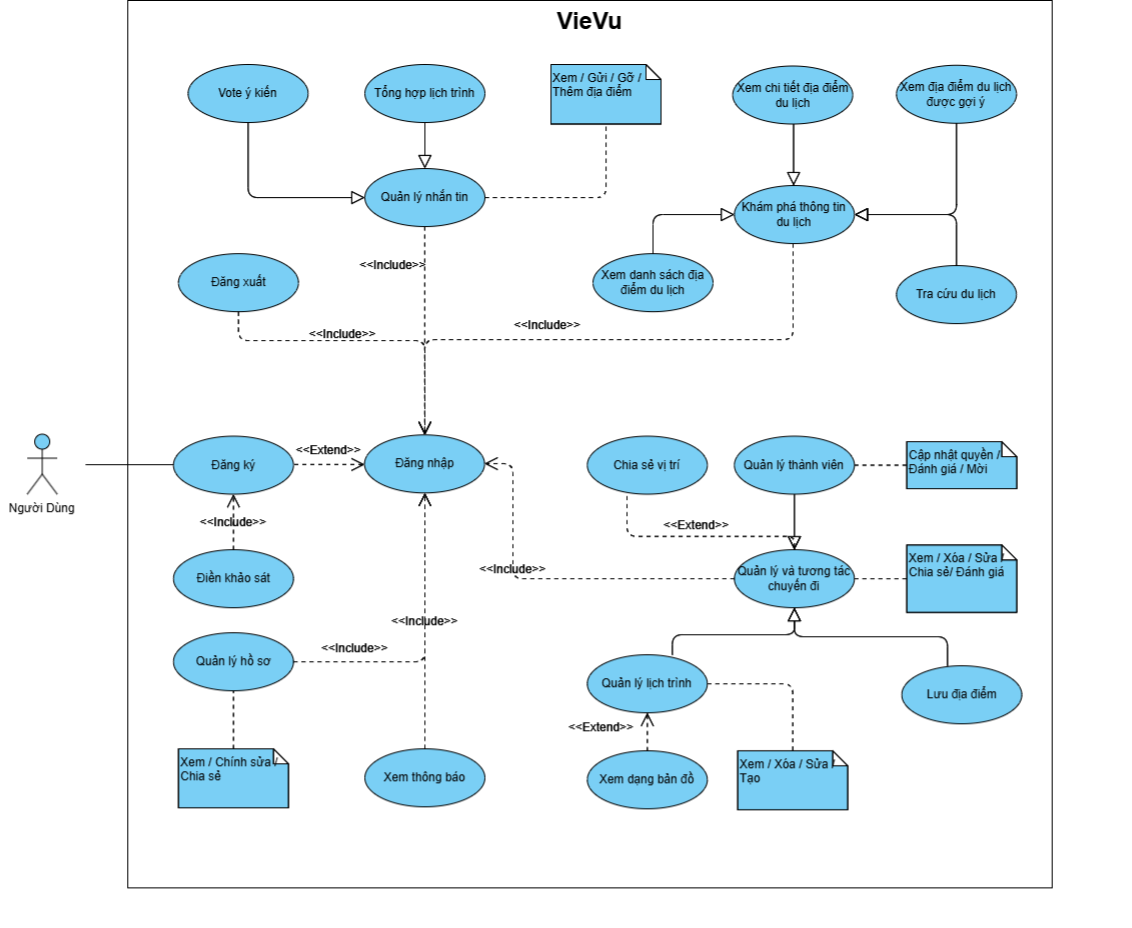
\includegraphics[width=1.1\textwidth]{figures/c3/3-2-usecases.png}
    \caption{Biểu đồ ca sử hệ thống.}
    \label{fig:3-2-usecases}
\end{figure}
\section{Mô tả ca sử dụng}

Phần này đi sâu vào mô tả chi tiết các ca sử dụng (use cases) chính của hệ thống VieVu. Mục tiêu là làm rõ cách thức người dùng tương tác với hệ thống để thực hiện các chức năng đã được xác định trong phần đặc tả yêu cầu. Mỗi ca sử dụng sẽ được trình bày theo một cấu trúc chuẩn hóa, bao gồm các yếu tố như tác nhân (actor), điều kiện tiên quyết (preconditions), luồng sự kiện chính (main flow), các luồng thay thế (alternative flows), và điều kiện kết thúc (postconditions). Việc phân tích và mô tả các ca sử dụng này không chỉ đảm bảo rằng tất cả các yêu cầu chức năng được bao phủ mà còn cung cấp một góc nhìn chi tiết về hoạt động của hệ thống từ quan điểm của người dùng cuối.

% \subsection{Ca sử dụng đăng ký}
\vspace{0.5cm}


\noindent 
\begin{tabularx}{\linewidth}{| l | X |} 
\hline 
\textbf{Mô tả} & Cho phép người dùng tạo một tài khoản trên ứng dụng để sử dụng các chức năng. \\ 
\hline 
\textbf{Luồng cơ bản} & 1. Người dùng truy cập màn hình đăng ký tài khoản. \newline
                       2. Ứng dụng hiển thị giao diện đăng ký tài khoản, yêu cầu người dùng nhập thông tin. \newline
                       3. Người dùng điền tên, email và mật khẩu của tài khoản muốn đăng ký. \newline
                       4. Người dùng nhấn đăng ký để hoàn thành quá trình. \newline
                       5. Hệ thống kiểm tra thông tin người dùng để trả về thông báo phù hợp và điều hướng người dùng đến màn hình điền khảo sát sở thích. \\ 
\hline 
\textbf{Luồng thay thế} &
                       - Nếu có lỗi tại server, hệ thống sẽ không lưu lại thông tin đã nhập vào. \newline
                       - Nếu thông tin nhập vào không hợp lệ sẽ thông báo lỗi để người dùng nhập lại. \\ 
\hline 
\textbf{Tiền điều kiện} & - Màn hình đăng ký đã hiển thị thành công trên ứng dụng. \newline
                       - Tài khoản email đúng định dạng và chưa được đăng ký trước đây. \\ 
\hline 
\textbf{Hậu điều kiện} & - Người đã đăng ký tài khoản có thể sử dụng nó để đăng nhập và thực hiện các chức năng với quyền hạn tương ứng. \newline
                       - Một hồ sơ người dùng và thông tin về sở thích được tạo và có thể được chỉnh sửa. \\ 
\hline 
\textbf{Yêu cầu phi chức năng} & Hệ thống xử lý đăng ký không quá 2s \\ 
\hline 
\end{tabularx}

\vspace{0.8cm}

\noindent 
\begin{tabular}{| c | c |}
    \hline
    \textbf{Biểu đồ hoạt động} & \textbf{Quan hệ} \\ 
    \hline
    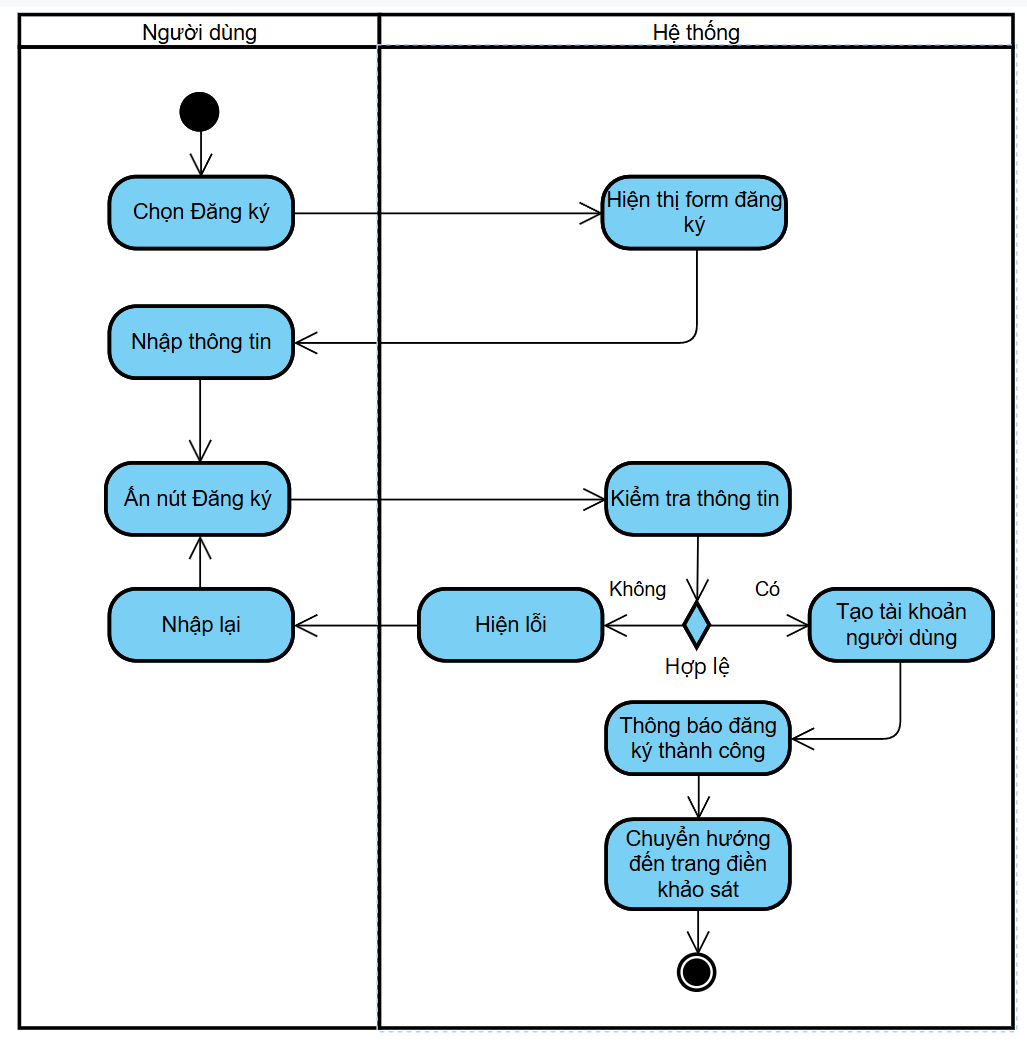
\includegraphics[width=0.5\linewidth]{figures/c3/3-3-1-ad.png} 
    & 
    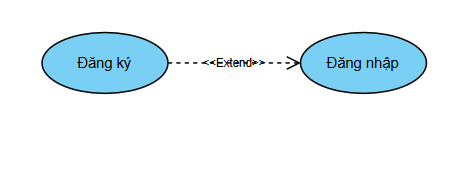
\includegraphics[width=0.45\linewidth]{figures/c3/3-3-1-rd.png} \\ 
    \hline
\end{tabular}

% \begin{figure}[H]
%     \centering  
%     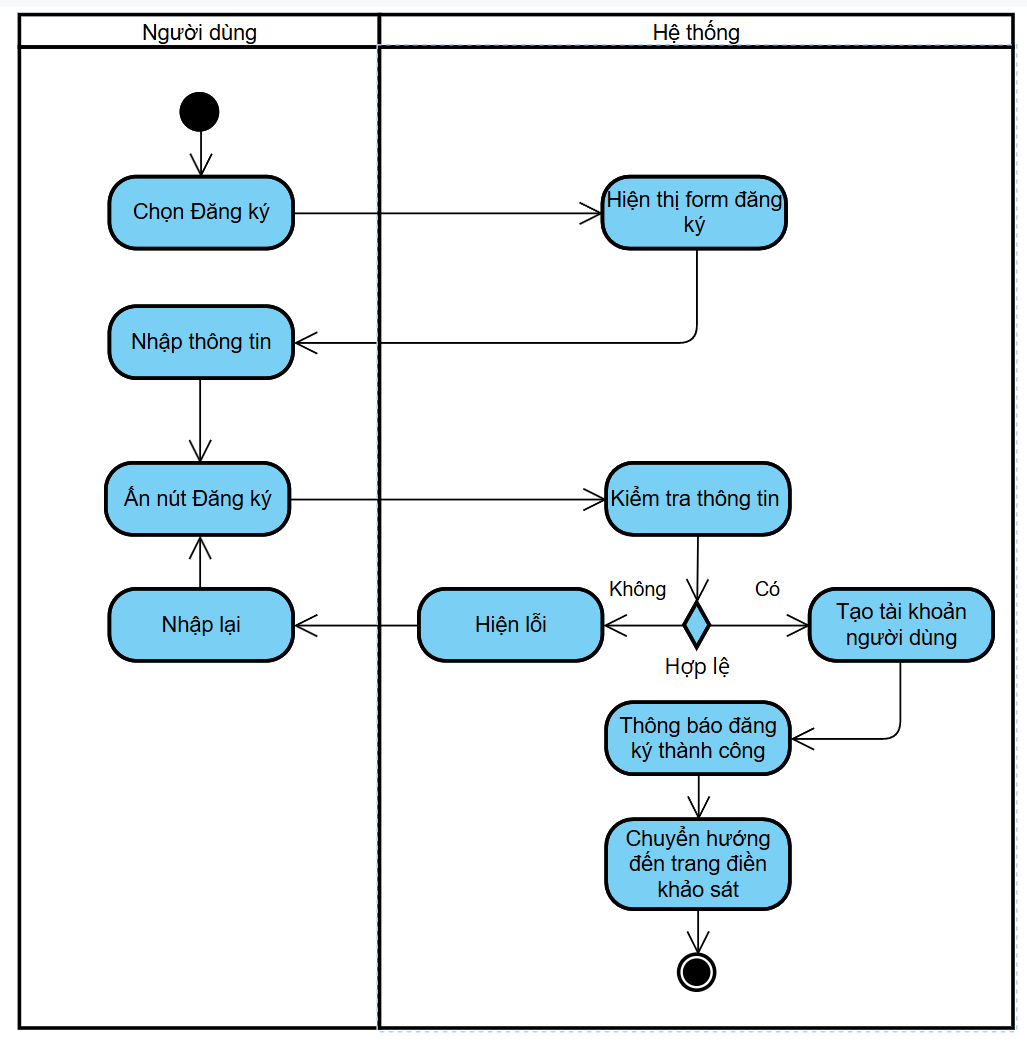
\includegraphics[width=0.5\textwidth]{figures/c3/3-3-1-ad.png}
%     \caption{Biểu đồ hoạt động ca sử dụng đăng ký.}
%     \label{fig:3-3-2-activity-diagram}
% \end{figure}



\begin{figure}[H]
    \centering  
    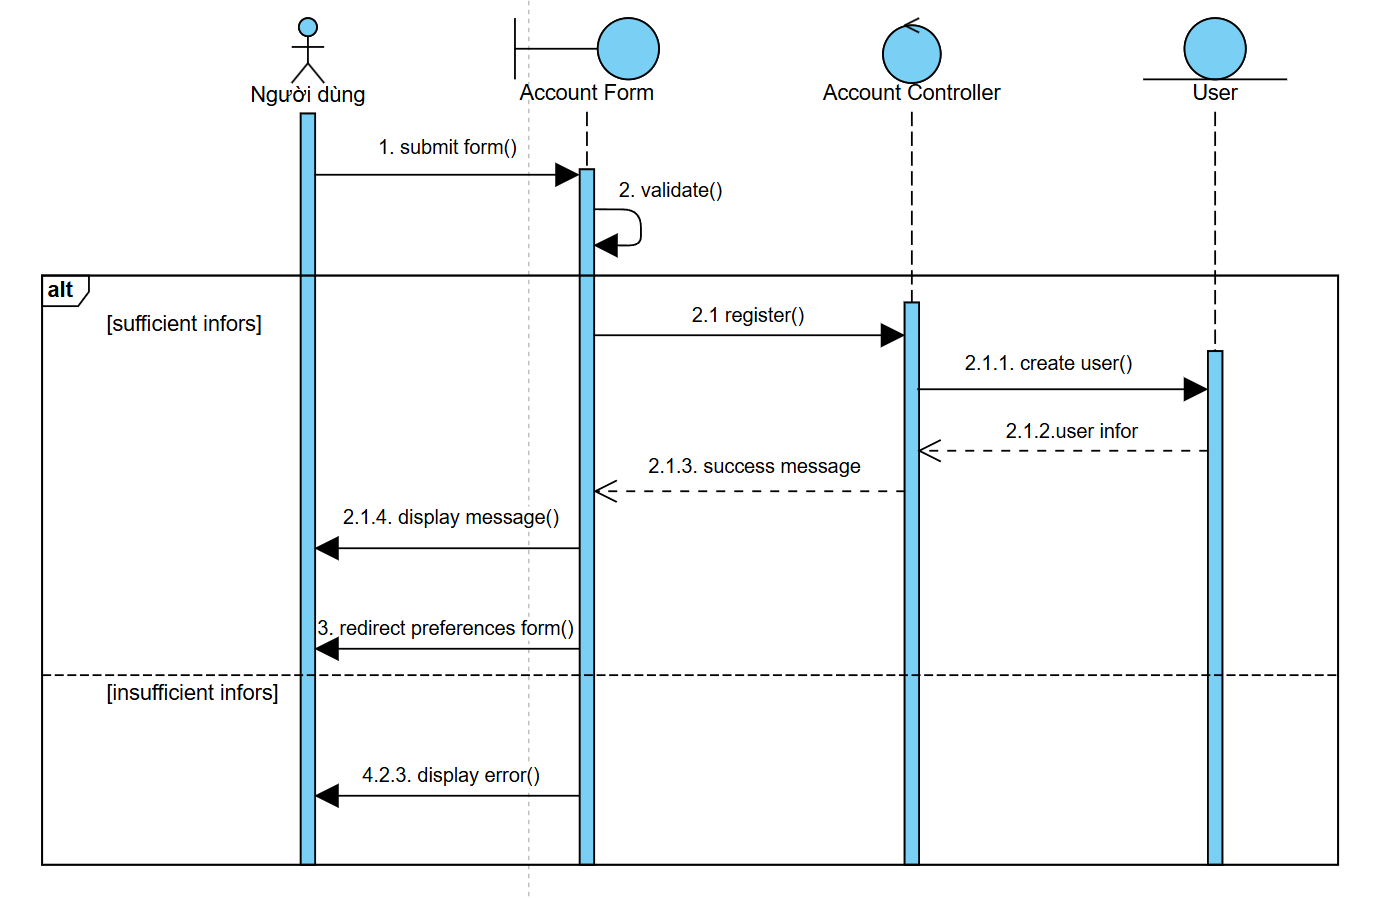
\includegraphics[width=1.05\textwidth]{figures/c3/3-3-1-sd.png}
    \caption{Biểu đồ tuần tự ca sử dụng đăng ký.}
    \label{fig:3-3-2-sequence-diagram}
\end{figure}
% \nopagebreak
% \subsection{Ca sử dụng đăng nhập}
\vspace{0.5cm}

\noindent 
\begin{tabularx}{\linewidth}{| l | X |} 
\hline 
\textbf{Mô tả} & Khi người dùng muốn sử dụng các chức năng yêu cầu quyền đăng nhập. \\ 
\hline 
\textbf{Luồng cơ bản} & 1. Truy cập trang đăng nhập \newline 
                      2. Nhập thông tin tài khoản (email / mật khẩu) \newline 
                      3. Điều hướng đến trang home - danh sách chuyến đi công khai. \\ 
\hline 
\textbf{Luồng thay thế} & - Nếu Người dùng nhập sai thông tin tài khoản hệ thống sẽ thông báo lỗi trên form đăng nhập  \newline 
                       - Người dùng có tài khoản chưa có thông tin sở thích hệ thống điều hướng đến trang khảo sát sở thích \\
\hline 
\textbf{Tiền điều kiện} & Người dùng đã đăng xuất. \\ 
\hline 
\textbf{Hậu điều kiện} & Hệ thống lưu token đăng nhập vào local trên thiết bị. \\ 
\hline 
\textbf{Yêu cầu phi chức năng} & Hệ thống xử lý đăng nhập không quá 2s. \\ 
\hline 
\end{tabularx}

\vspace{0.8cm}

\noindent 
\begin{tabular}{| c | c |}
    \hline
    \textbf{Biểu đồ hoạt động} & \textbf{Quan hệ} \\ 
    \hline
    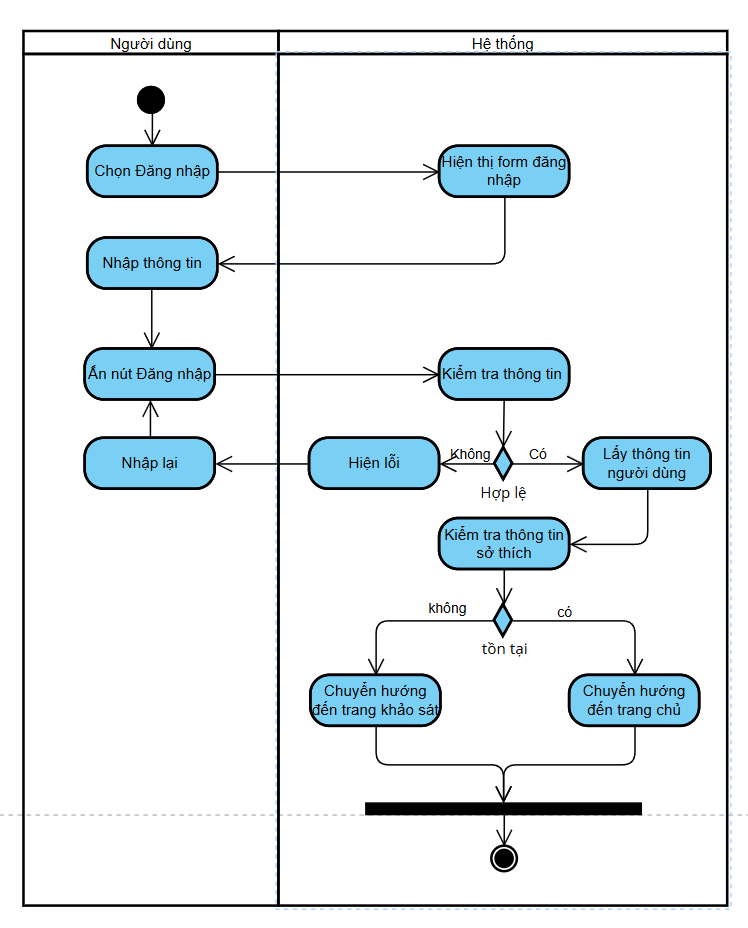
\includegraphics[width=0.5\linewidth]{figures/c3/3-3-2-ad.png} 
    & 
    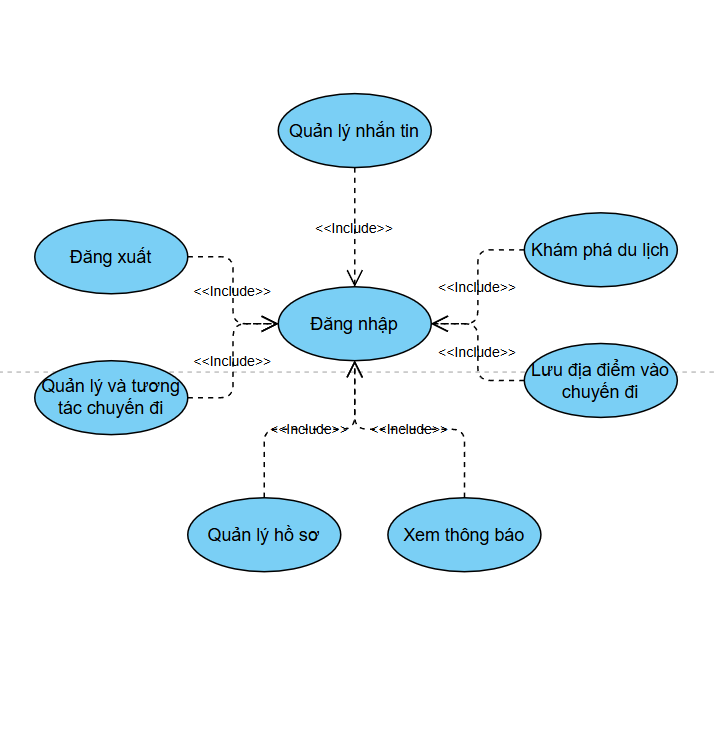
\includegraphics[width=0.45\linewidth]{figures/c3/3-3-2-rd.png} \\ 
    \hline
\end{tabular}
\vspace{0.8cm}

\begin{figure}[H]
    \centering  
    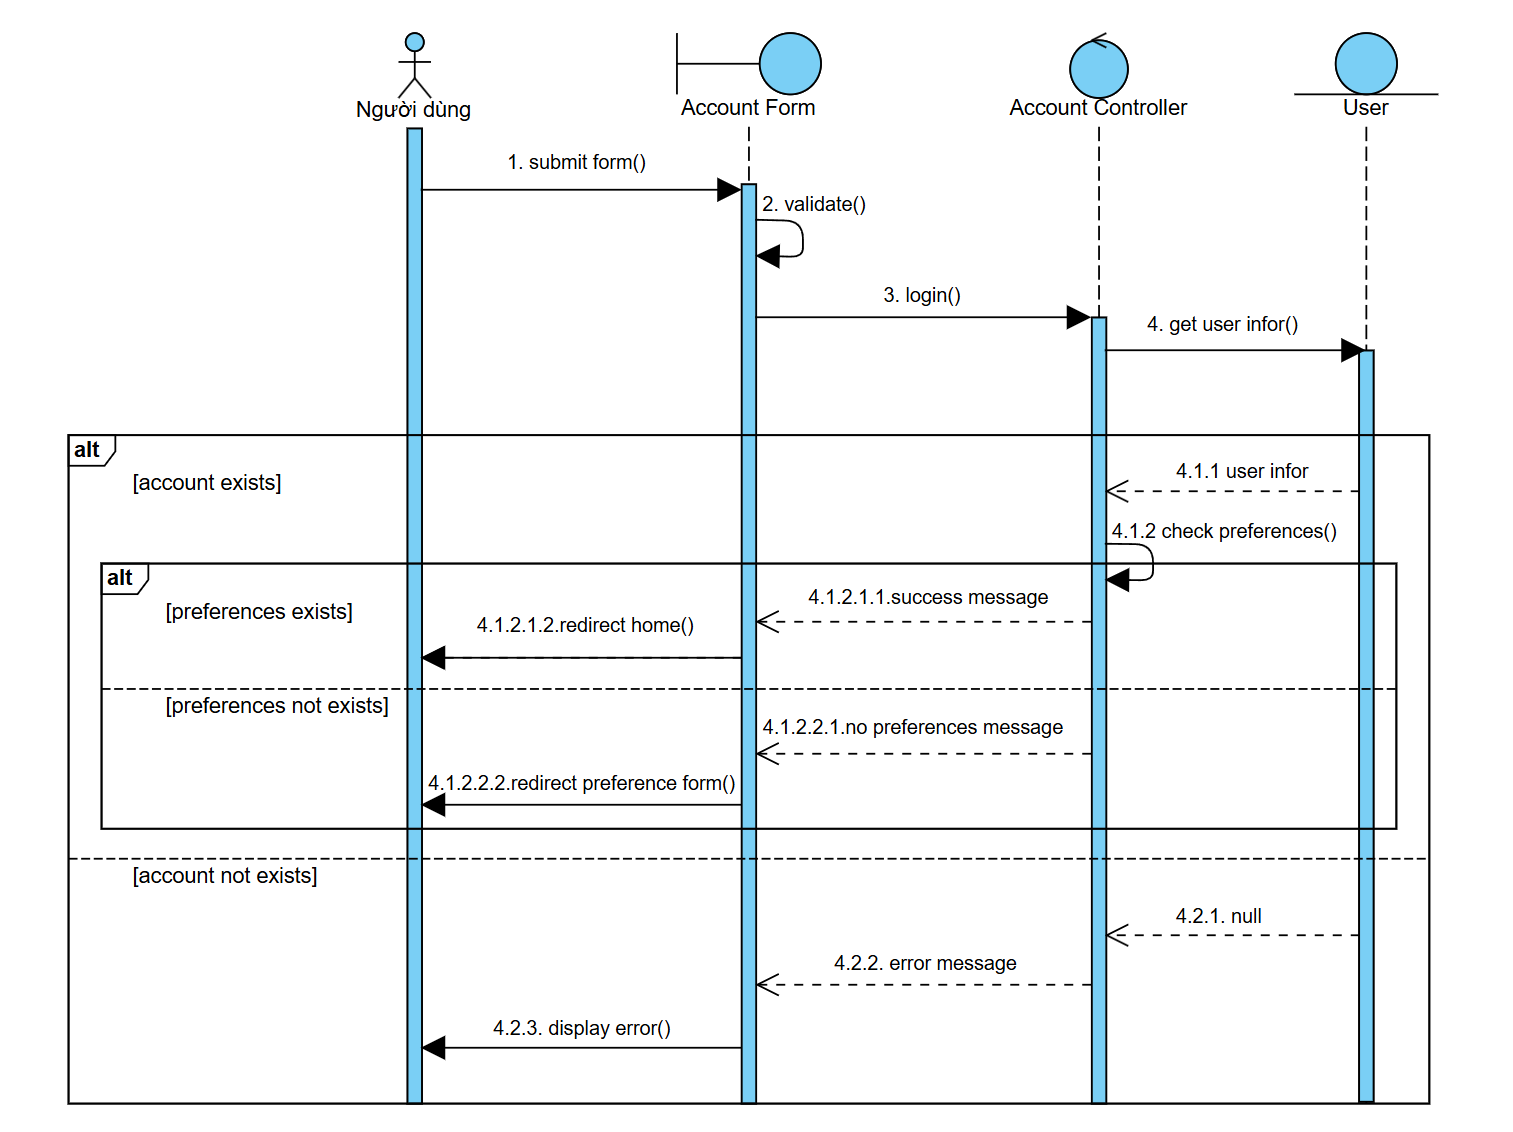
\includegraphics[width=1.05\textwidth]{figures/c3/3-3-2-sd.png}
    \caption{Biểu đồ tuần tự ca sử dụng đăng nhập.}
    \label{fig:3-3-1-sequence-diagram}
\end{figure}
% \nopagebreak
% \subsection{Ca sử dụng điền khảo sát sở thích}
\noindent Ca sử dụng này mô tả quá trình người dùng cung cấp thông tin về sở thích du lịch của mình sau khi đăng ký tài khoản. Thông tin này sẽ được hệ thống sử dụng để cá nhân hóa các gợi ý và trải nghiệm trong ứng dụng. Bảng~\ref{tab:uc_survey_spec} trình bày chi tiết đặc tả ca sử dụng, bao gồm luồng sự kiện chính, các điều kiện và yêu cầu liên quan. Các biểu đồ hoạt động, quan hệ (Bảng~\ref{tab:uc_survey_diagrams}) và tuần tự (Hình~\ref{fig:3-3-3-sequence-diagram}) minh họa rõ hơn về quy trình và tương tác hệ thống.

\begin{longtable}{| p{4cm} | p{\dimexpr\linewidth-4cm-4\tabcolsep} |} % Adjust widths as needed
    \caption{Đặc tả ca sử dụng điền khảo sát sở thích.} % Caption inside longtable
    \label{tab:uc_survey_spec} \\ % Label after caption

    \hline
    \textbf{Mô tả} & Người dùng cập nhật thông tin về sở thích du lịch của bản thân để sử dụng dịch vụ gợi ý trong ứng dụng \\
    \hline
    \endfirsthead % Header for the first page

    \hline
 
    \textbf{Mô tả} & Người dùng cập nhật thông tin về sở thích du lịch của bản thân để sử dụng dịch vụ gợi ý trong ứng dụng. \\
    \hline
    \endhead

    \hline 
    \endfoot

    \hline % Footer for the last page
    \endlastfoot

    \textbf{Luồng cơ bản} & 1. Người dùng đăng ký tài khoản mới \newline
                           2. Ứng dụng hiển thị các form lựa chọn lần lượt theo loại hình du lịch, giá tiền,v.v. \newline
                           3. Người dùng chọn các loại hình du lịch theo sở thích. \newline
                           4. Người dùng chọn khoảng giá du lịch phù hợp với bản thân. \newline
                           5. Người dùng nhấn nút hoàn tất để hoàn thành quá trình. \newline
                           6. Hệ thống điều hướng người dùng đến trang chủ của ứng dụng. \\
    \hline
    \textbf{Tiền điều kiện} & Người dùng đăng ký tài khoản thành công và chưa hoàn thành điền khảo sát sở thích. \\
    \hline
    \textbf{Hậu điều kiện} & Thông tin sở thích được lưu lại trong cơ sở dữ liệu. \\
    \hline
    \textbf{Yêu cầu phi chức năng} & Hệ thống xử lý cập nhật không quá 1s \\

\end{longtable}

\begin{table}[H] % Add table environment
    \centering
    \caption{Biểu đồ hoạt động và quan hệ ca sử dụng điền khảo sát sở thích} % Add caption
    \label{tab:uc_survey_diagrams} % Add label
    \begin{tabular}{| c | c |}
        \hline
        \textbf{Biểu đồ hoạt động} & \textbf{Quan hệ} \\
        \hline
        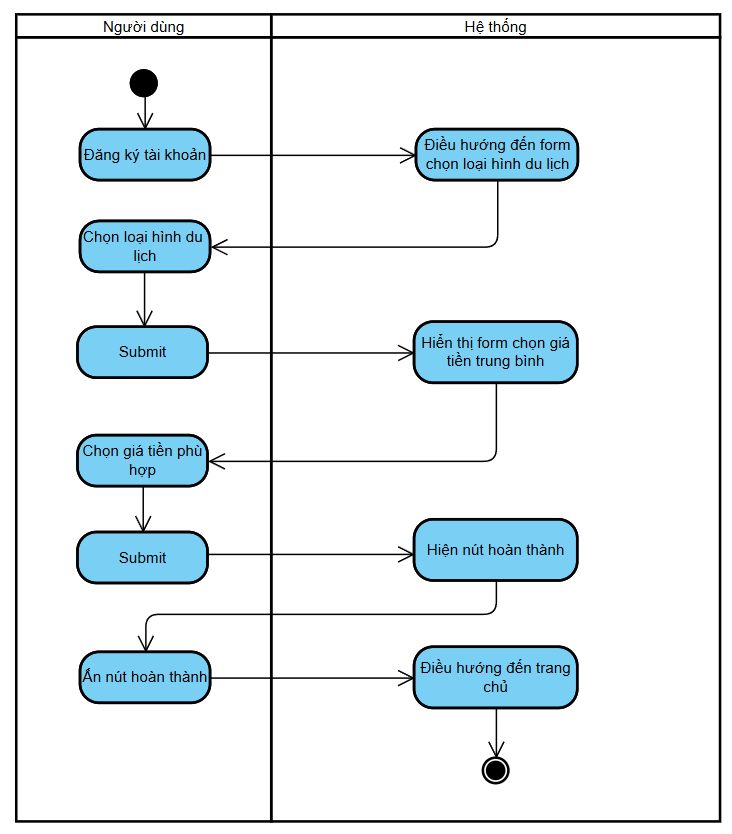
\includegraphics[width=0.5\linewidth]{figures/c3/3-3-3-ad.png}
        &
        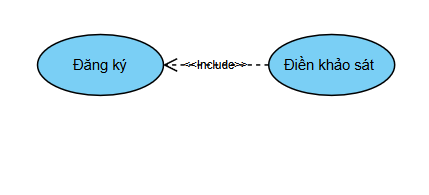
\includegraphics[width=0.45\linewidth]{figures/c3/3-3-3-rd.png} \\
        \hline
    \end{tabular}
\end{table}


\begin{figure}[H]
    \centering
    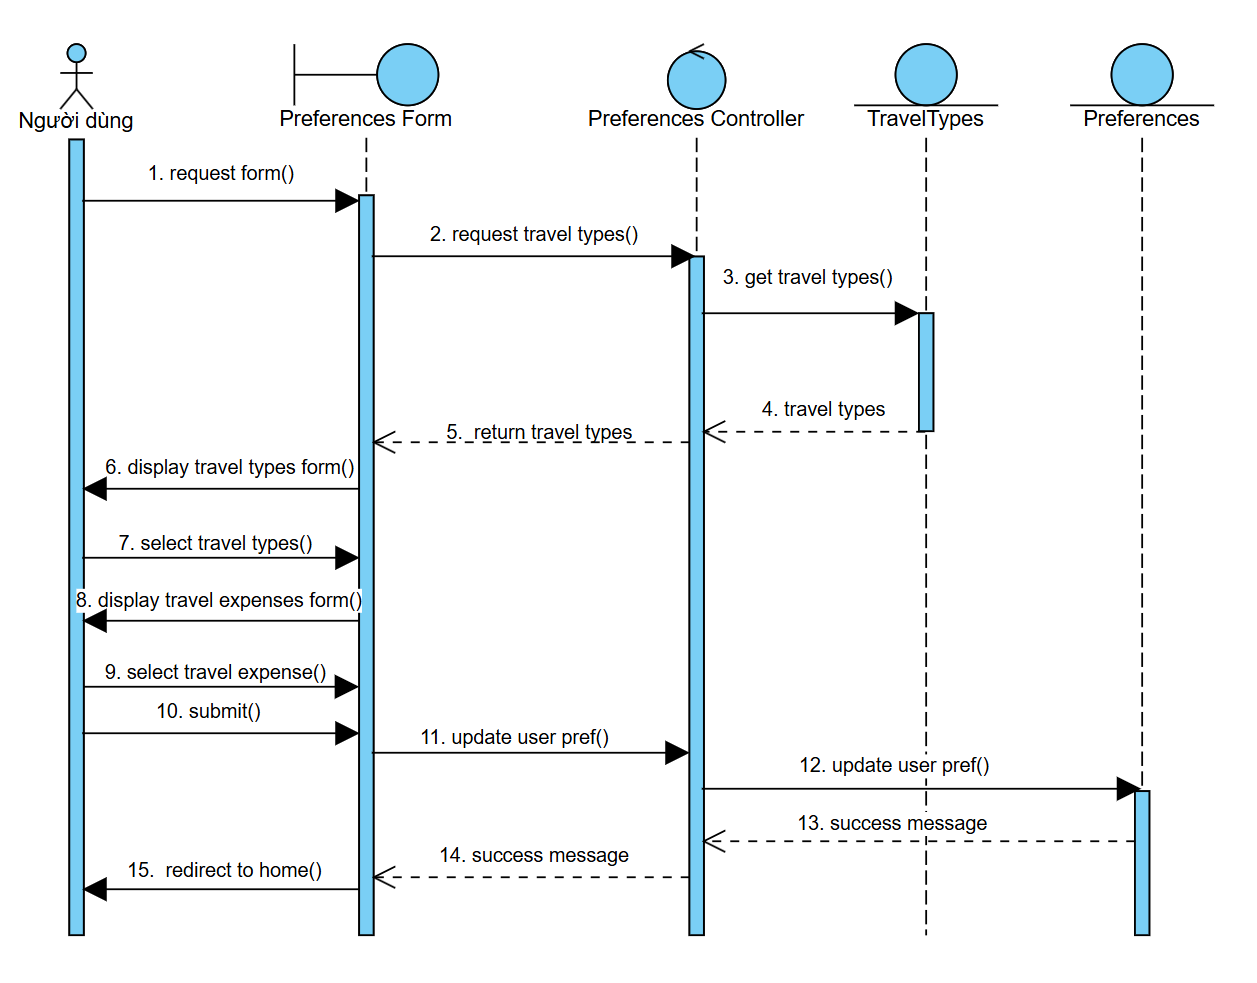
\includegraphics[width=0.85\textwidth]{figures/c3/3-3-3-sd.png}
    \caption{Biểu đồ tuần tự ca sử dụng điền khảo sát sở thích.}
    \label{fig:3-3-3-sequence-diagram}
\end{figure}
% \nopagebreak
% \subsection{Ca sử dụng chỉnh sửa thông tin cá nhân}
\vspace{0.5cm}


\noindent 
\begin{tabularx}{\linewidth}{| l | X |} 
\hline 
\textbf{Mô tả} & Người dùng cập nhật thông tin cá nhân như
địa chỉ, tên, số điện thoại, mô tả, ảnh đại diện,v.v. \\ 
\hline 
\textbf{Luồng cơ bản} & 1. Người dùng truy cập tab tài khoản và bấm vào trang hồ sơ của bản thân \newline
                       2. Người dùng ấn vào nút chính sửa \newline
                       3. Người dùng nhập các thông tin cần thay đổi. \newline
                       5. Người dùng ấn nút submit. \newline
                       6. Hệ thống cập nhật thông tin người dùng và thông báo cập nhật thành công. \\
\hline 
\textbf{Luồng thay thế} & Nếu Người dùng nhập thông tin không hợp lệ hệ thống sẽ báo lỗi. \\
\hline 
\textbf{Tiền điều kiện} & Người dùng đang đăng nhập và phiên đăng nhập chưa kết thúc. \\
\hline 
\textbf{Hậu điều kiện} & Thông tin mới của người dùng được cập nhật. \\

\hline 
\textbf{Yêu cầu phi chức năng} & Hệ thống xử lý cập nhật không quá 5s (do có upload ảnh) \\ 
\hline 
\end{tabularx}

\vspace{0.8cm}

\noindent 
\begin{tabular}{| c | c |}
    \hline
    \textbf{Biểu đồ hoạt động} & \textbf{Quan hệ} \\ 
    \hline
    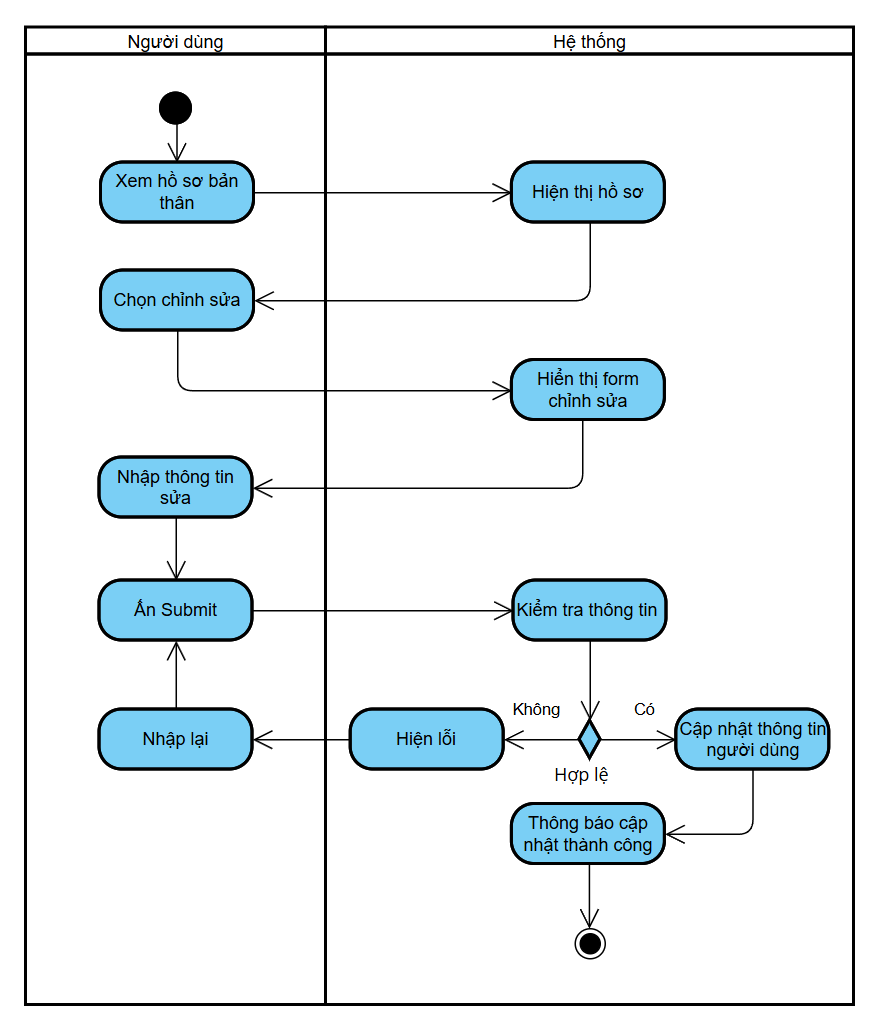
\includegraphics[width=0.5\linewidth]{figures/c3/3-3-4-ad.png} 
    & 
    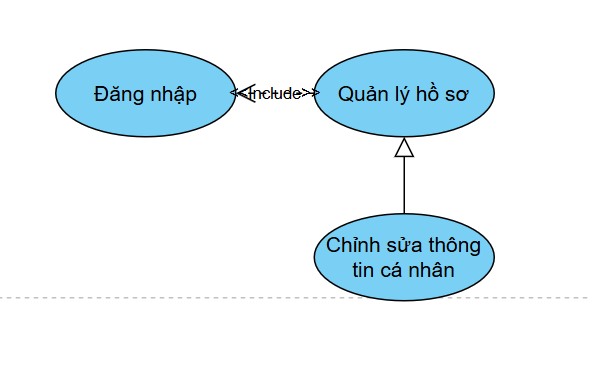
\includegraphics[width=0.45\linewidth]{figures/c3/3-3-4-rd.png} \\ 
    \hline
\end{tabular}



\begin{figure}[H]
    \centering  
    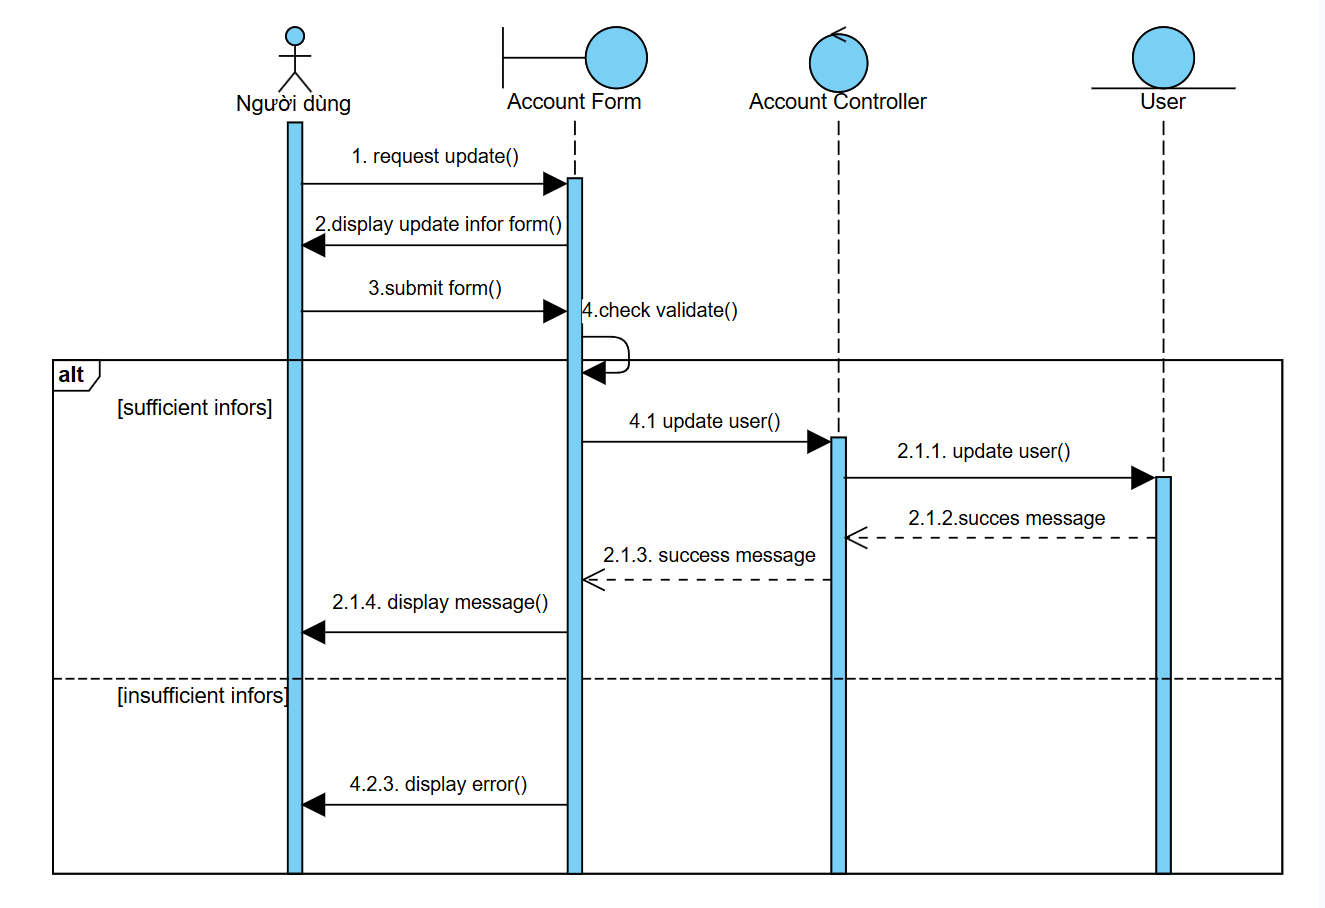
\includegraphics[width=1\textwidth]{figures/c3/3-3-4-sd.png}
    \caption{Biểu đồ tuần tự ca sử dụng chỉnh sửa thông tin cá nhân.}
    \label{fig:3-3-4-sequence-diagram}
\end{figure}
% \nopagebreak
\subsection{Ca sử dụng tra cứu du lịch}
\noindent Ca sử dụng này mô tả quá trình người dùng tìm kiếm thông tin về các địa điểm du lịch, sự kiện, hoặc các dịch vụ khác thông qua chức năng tìm kiếm của ứng dụng. Người dùng có thể nhập từ khóa và áp dụng các bộ lọc để thu hẹp kết quả. Bảng~\ref{tab:uc_search_spec} trình bày chi tiết đặc tả ca sử dụng, bao gồm luồng sự kiện chính, các điều kiện và yêu cầu liên quan. Các biểu đồ hoạt động, quan hệ (Bảng~\ref{tab:uc_search_diagrams}) và tuần tự (Hình~\ref{fig:3-3-5-sequence-diagram}) minh họa rõ hơn về quy trình và tương tác hệ thống khi người dùng thực hiện tra cứu.
% \vspace{0.5cm} % Adjust spacing if needed

% Use longtable environment
% Need \usepackage{longtable} and \usepackage{calc} in preamble
\begin{longtable}{| p{4cm} | p{\dimexpr\linewidth-4cm-4\tabcolsep} |} % Adjust widths as needed
    \caption{Đặc tả ca sử dụng tra cứu du lịch} % Caption inside longtable
    \label{tab:uc_search_spec} \\ % Label after caption

    \hline
    \textbf{Mô tả} & Người dùng tra cứu và lọc tên địa điểm du lịch, sự kiện, điểm đến muốn tìm hiểu. \\
    \hline
    \endfirsthead % Header for the first page

    \hline
    % \multicolumn{2}{|c|}{(Tiếp theo)} \\ % Header for subsequent pages
    % \hline
    \textbf{Mô tả} & Người dùng tra cứu và lọc tên địa điểm du lịch, sự kiện, điểm đến muốn tìm hiểu. \\
    \hline
    \endhead

    \hline 
    % \multicolumn{2}{|r|}{{Tiếp tục ở trang sau}} \\ % Footer for pages before the last
    \endfoot

    \hline % Footer for the last page
    \endlastfoot

    % --- Table Content ---
    \textbf{Luồng cơ bản} & 1. Người dùng truy cập tab khám phá và bấm vào thanh tìm kiếm. \newline
                           2. Hệ thống hiển thị lịch sử tìm kiếm và các bộ lọc. \newline
                           3. Người dùng nhập từ khóa tìm kiếm. \newline
                           4. Người dùng chọn bộ lọc (sự kiện, địa điểm, nhà hàng, khách sạn, điểm đến, v.v.). \newline
                           5. Hệ thống tra cứu, lưu từ khóa tìm kiếm và hiển thị kết quả theo danh sách. \\
    \hline
    % \textbf{Luồng thay thế} & (Nếu có luồng thay thế, thêm vào đây) \\
    % \hline
    \textbf{Tiền điều kiện} & Người dùng đang đăng nhập và phiên đăng nhập chưa kết thúc. \\
    \hline
    \textbf{Hậu điều kiện} & - Người dùng có thể xem thông tin về các kết quả tìm kiếm.\newline
                           - Hệ thống lưu lại lịch sử tìm kiếm của người dùng. \newline
                           - Hệ thống có thể cập nhật sở thích của người dùng dựa trên từ khóa tìm kiếm. \\
    \hline
    \textbf{Yêu cầu phi chức năng} & Hệ thống xử lý tìm kiếm không quá 2 giây. \\
    % --- End Table Content ---

\end{longtable}
% \vspace{0.8cm}

\begin{table}[H] % Wrap the diagrams table
    \centering
    \caption{Biểu đồ hoạt động và quan hệ ca sử dụng tra cứu du lịch} % Add caption
    \label{tab:uc_search_diagrams} % Add label
    \begin{tabular}{| c | c |}
        \hline
        \textbf{Biểu đồ hoạt động} & \textbf{Quan hệ} \\
        \hline
        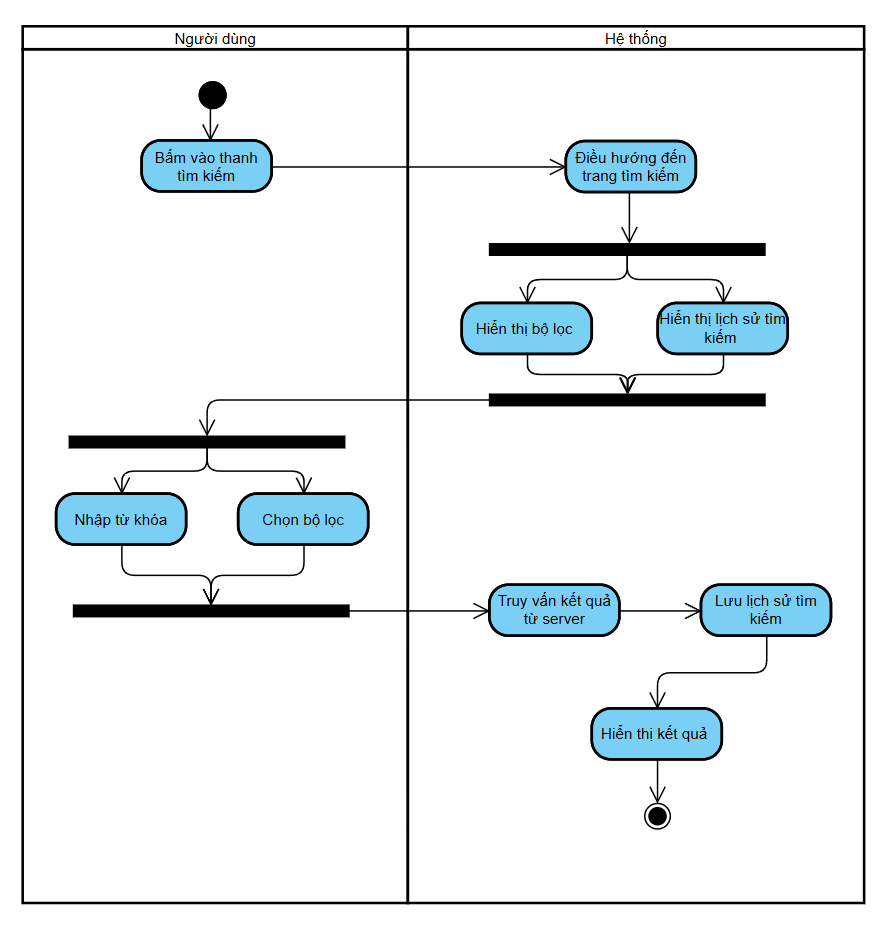
\includegraphics[width=0.5\linewidth]{figures/c3/3-3-5-ad.png}
        &
        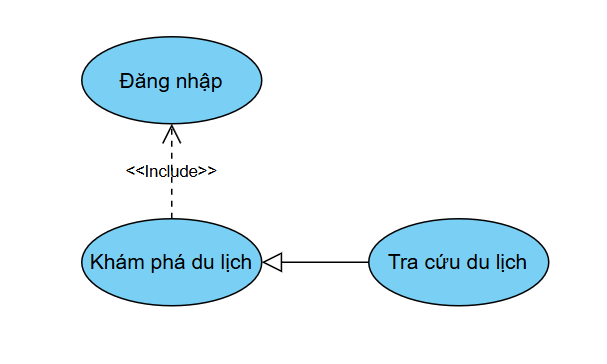
\includegraphics[width=0.45\linewidth]{figures/c3/3-3-5-rd.png} \\
        \hline
    \end{tabular}
\end{table}

\begin{figure}[H]
    \centering
    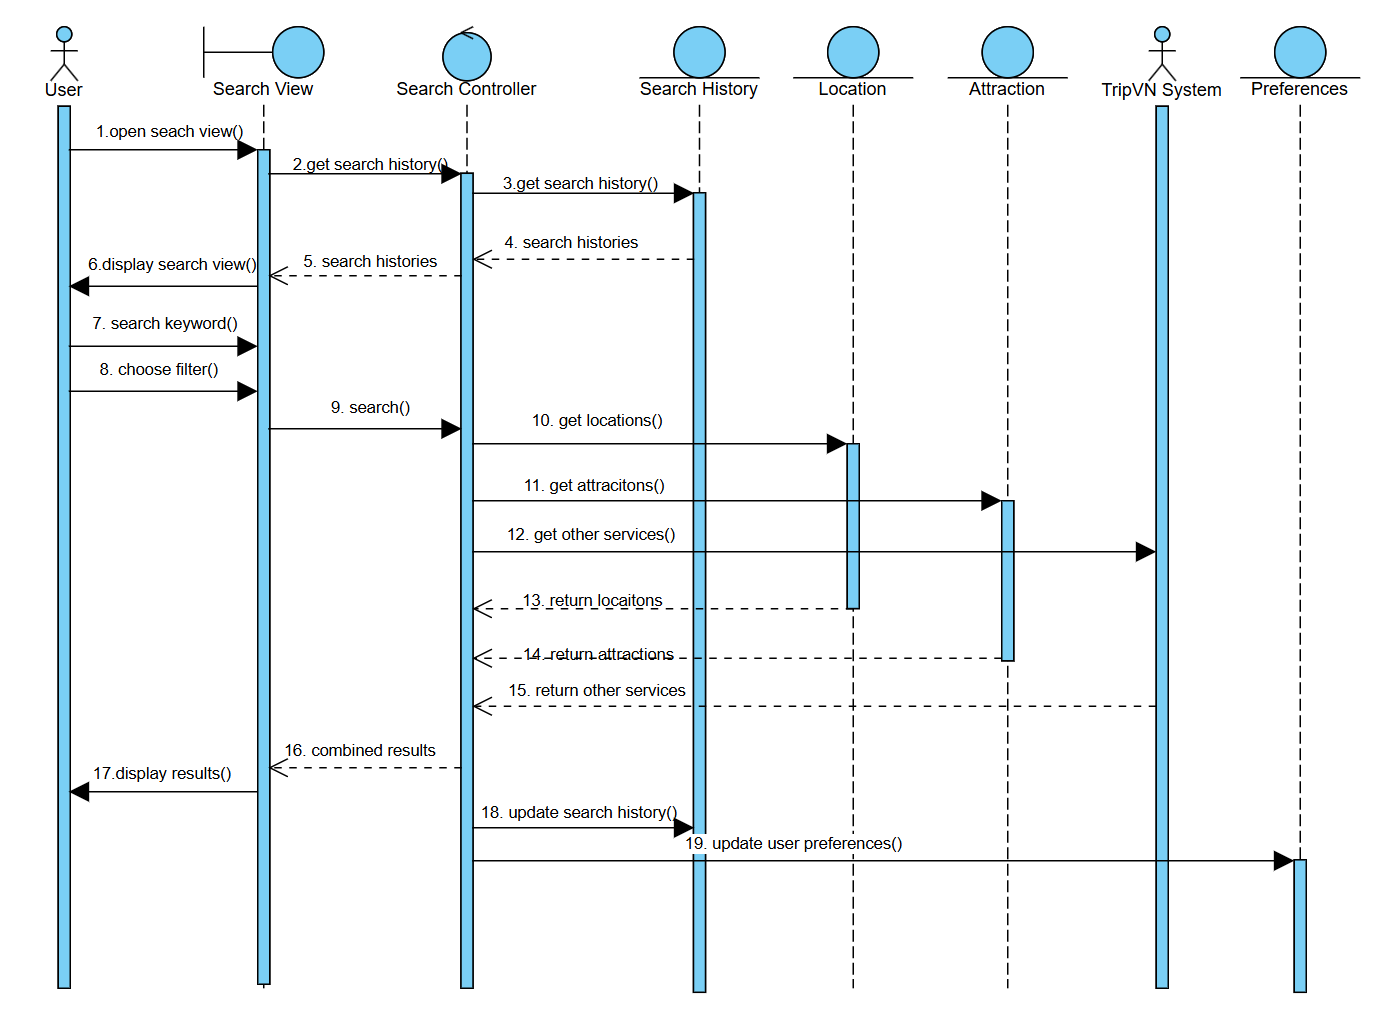
\includegraphics[width=1\textwidth]{figures/c3/3-3-5-sd.png} % Adjusted width slightly
    \caption{Biểu đồ tuần tự ca sử dụng tra cứu du lịch.}
    \label{fig:3-3-5-sequence-diagram}
\end{figure}
\nopagebreak
\subsection{Ca sử dụng xem danh sách địa điểm được gợi ý}
\noindent Ca sử dụng này mô tả cách người dùng xem danh sách các địa điểm du lịch được hệ thống gợi ý dựa trên sở thích cá nhân. Người dùng cũng có thể tùy chỉnh các bộ lọc sở thích để nhận được những gợi ý khác phù hợp hơn. Bảng~\ref{tab:uc_view_recommendations_spec} trình bày chi tiết đặc tả ca sử dụng, bao gồm luồng sự kiện chính, luồng thay thế, các điều kiện và yêu cầu liên quan. Các biểu đồ hoạt động, quan hệ (Bảng~\ref{tab:uc_view_recommendations_diagrams}) và tuần tự (Hình~\ref{fig:3-3-6-sequence-diagram}) minh họa rõ hơn về quy trình và tương tác hệ thống khi người dùng xem các gợi ý.
% \vspace{0.5cm} % Adjust spacing if needed

% Use longtable environment
% Need \usepackage{longtable} and \usepackage{calc} in preamble
\begin{longtable}{| p{4cm} | p{\dimexpr\linewidth-4cm-4\tabcolsep} |} % Adjust widths as needed
    \caption{Đặc tả ca sử dụng xem danh sách địa điểm được gợi ý} % Caption inside longtable
    \label{tab:uc_view_recommendations_spec} \\ % Label after caption

    \hline
    \textbf{Mô tả} & Người dùng xem danh sách địa điểm du lịch gợi ý cho bản thân và tùy chỉnh sở thích về loại hình du lịch để lấy gợi ý khác. \\
    \hline
    \endfirsthead % Header for the first page

    % No \endhead content needed

    % No \endfoot content needed

    \hline % Footer for the last page
    \endlastfoot

    % --- Table Content ---
    \textbf{Luồng cơ bản} & 1. Người dùng truy cập tab khám phá. \newline
                           2. Người dùng bấm vào trang đề xuất địa điểm du lịch. \newline
                           3. Hệ thống điều hướng đến trang hiển thị danh sách địa điểm du lịch gợi ý cho người dùng và bộ lọc tùy chỉnh. \\
    \hline
    \textbf{Luồng thay thế} & Người dùng tùy chỉnh bộ lọc sở thích loại hình du lịch để nhận gợi ý khác. \\
    \hline
    \textbf{Tiền điều kiện} & - Người dùng đang đăng nhập và phiên đăng nhập chưa kết thúc. \newline
                             - Người dùng có thông tin về sở thích. \\
    \hline
    \textbf{Hậu điều kiện} & - Người dùng có thể chọn địa điểm trong danh sách để xem chi tiết. \\
    \hline
    \textbf{Yêu cầu phi chức năng} & Hệ thống xử lý lấy danh sách không quá 2s. \\
    % --- End Table Content ---

\end{longtable}
\vspace{0.8cm}

\begin{table}[H] % Wrap the diagrams table
    \centering
    \caption{Biểu đồ hoạt động ca sử dụng xem danh sách địa điểm được gợi ý} % Add caption
    \label{tab:uc_view_recommendations_diagrams} % Add label
    \begin{tabular}{| c | c |}
        \hline
        \textbf{Biểu đồ hoạt động} & \textbf{Quan hệ} \\
        \hline
        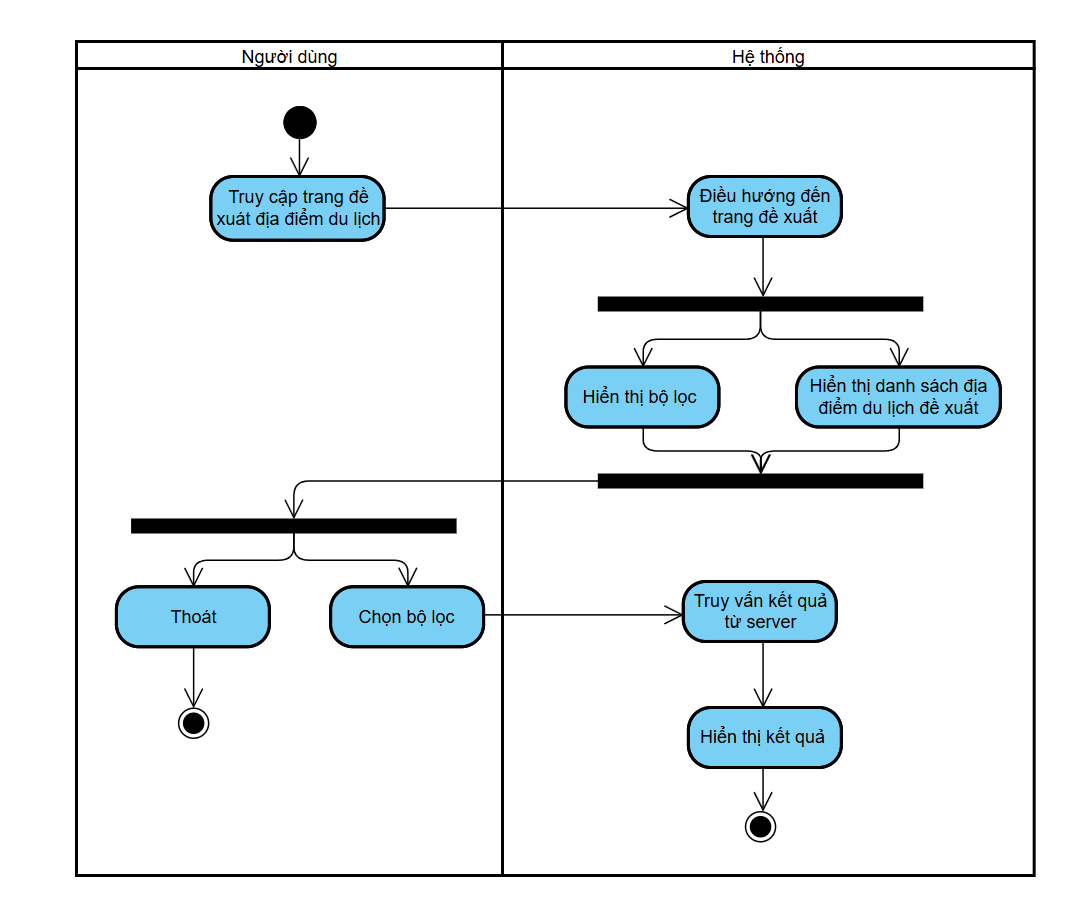
\includegraphics[width=0.5\linewidth]{figures/c3/3-3-6-ad.png}
        &
        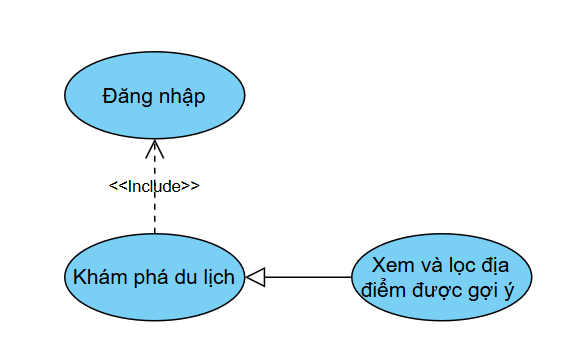
\includegraphics[width=0.45\linewidth]{figures/c3/3-3-6-rd.png} \\
        \hline
    \end{tabular}
\end{table}

\begin{figure}[H]
    \centering
    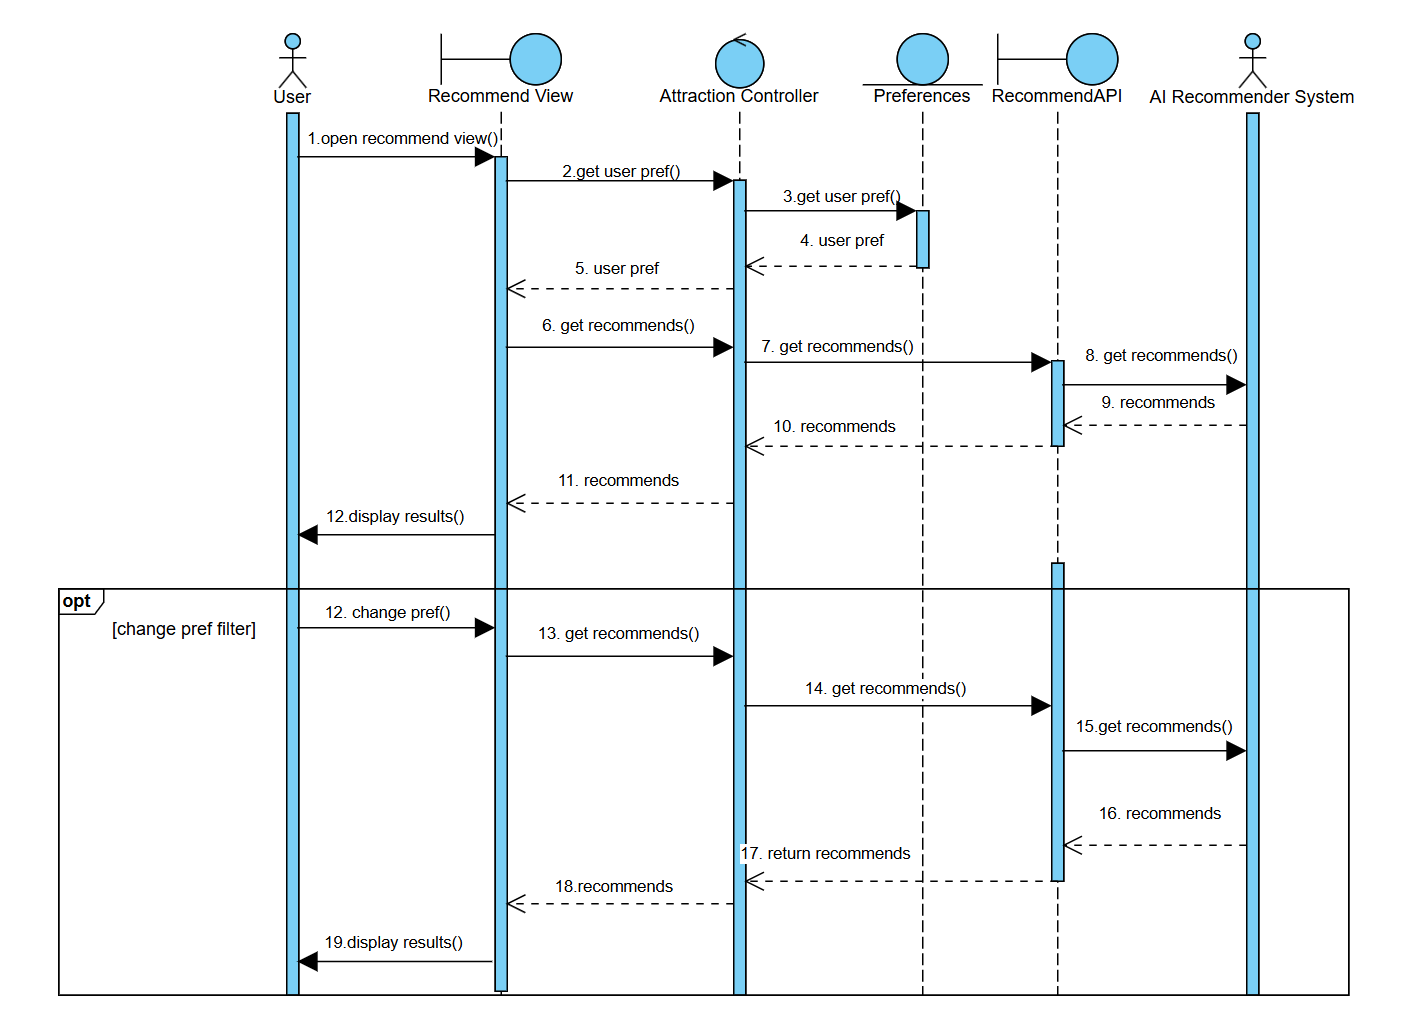
\includegraphics[width=1\textwidth]{figures/c3/3-3-6-sd.png} % Adjusted width slightly
    \caption{Biểu đồ tuần tự ca sử dụng xem danh sách địa điểm được gợi ý.}
    \label{fig:3-3-6-sequence-diagram}
\end{figure}
\nopagebreak
\subsection{Ca sử dụng xem danh sách địa điểm gần người dùng}
\noindent Ca sử dụng này mô tả cách người dùng tìm kiếm và xem danh sách các địa điểm (du lịch, nhà hàng, khách sạn) ở gần vị trí hiện tại của họ. Hệ thống yêu cầu quyền truy cập vị trí để thực hiện chức năng này. Bảng~\ref{tab:uc_nearby_places_spec} trình bày chi tiết đặc tả ca sử dụng, bao gồm luồng sự kiện chính, luồng thay thế, các điều kiện và yêu cầu liên quan. Các biểu đồ hoạt động, quan hệ (Bảng~\ref{tab:uc_nearby_places_diagrams}) và tuần tự (Hình~\ref{fig:3-3-7-sequence-diagram}) minh họa rõ hơn về quy trình và tương tác hệ thống.
% \vspace{0.5cm} % Adjust spacing if needed

% Use longtable environment
% Need \usepackage{longtable} and \usepackage{calc} in preamble
\begin{longtable}{| p{4cm} | p{\dimexpr\linewidth-4cm-4\tabcolsep} |} % Adjust widths as needed
    \caption{Đặc tả ca sử dụng xem danh sách địa điểm gần người dùng} % Caption inside longtable
    \label{tab:uc_nearby_places_spec} \\ % Label after caption

    \hline
    \textbf{Mô tả} & Người dùng xem danh sách địa điểm du lịch, nhà hàng, khách sạn gần bản thân. \\
    \hline
    \endfirsthead % Header for the first page

    % No \endhead content needed

    % No \endfoot content needed

    \hline % Footer for the last page
    \endlastfoot

    % --- Table Content ---
    \textbf{Luồng cơ bản} & 1. Người dùng truy cập tab khám phá và bấm vào thanh tìm kiếm. \newline
                           2. Người dùng bấm vào biểu tượng ``Lân cận". \newline
                           3. Hệ thống hiển thị hộp thoại cấp quyền thông tin vị trí hiện tại. \newline
                           4. Người dùng cấp quyền cho hệ thống. \newline
                           5. Hệ thống lấy vị trí hiện tại của người dùng và hiển thị danh sách địa điểm gần nhất. \\
    \hline
    \textbf{Luồng thay thế} & Người dùng không cấp quyền truy cập vị trí sẽ nhận thông báo lỗi. \\
    \hline
    \textbf{Tiền điều kiện} & Người dùng đang đăng nhập và phiên đăng nhập chưa kết thúc. \\
    \hline
    \textbf{Hậu điều kiện} & - Người dùng có thể xem địa chỉ của bản thân và xem chi tiết các dịch vụ, địa điểm trong danh sách. \newline
                           - Người dùng có thể xem dạng bản đồ các địa điểm trong danh sách. \\
    \hline
    \textbf{Yêu cầu phi chức năng} & Hệ thống xử lý lấy danh sách không quá 5s. \\
    % --- End Table Content ---

\end{longtable}
\vspace{0.8cm}

\begin{table}[H] % Wrap the diagrams table
    \centering
    \caption{Biểu đồ hoạt động ca sử dụng xem danh sách địa điểm gần người dùng} % Add caption
    \label{tab:uc_nearby_places_diagrams} % Add label
    \begin{tabular}{| c | c |}
        \hline
        \textbf{Biểu đồ hoạt động} & \textbf{Quan hệ} \\
        \hline
        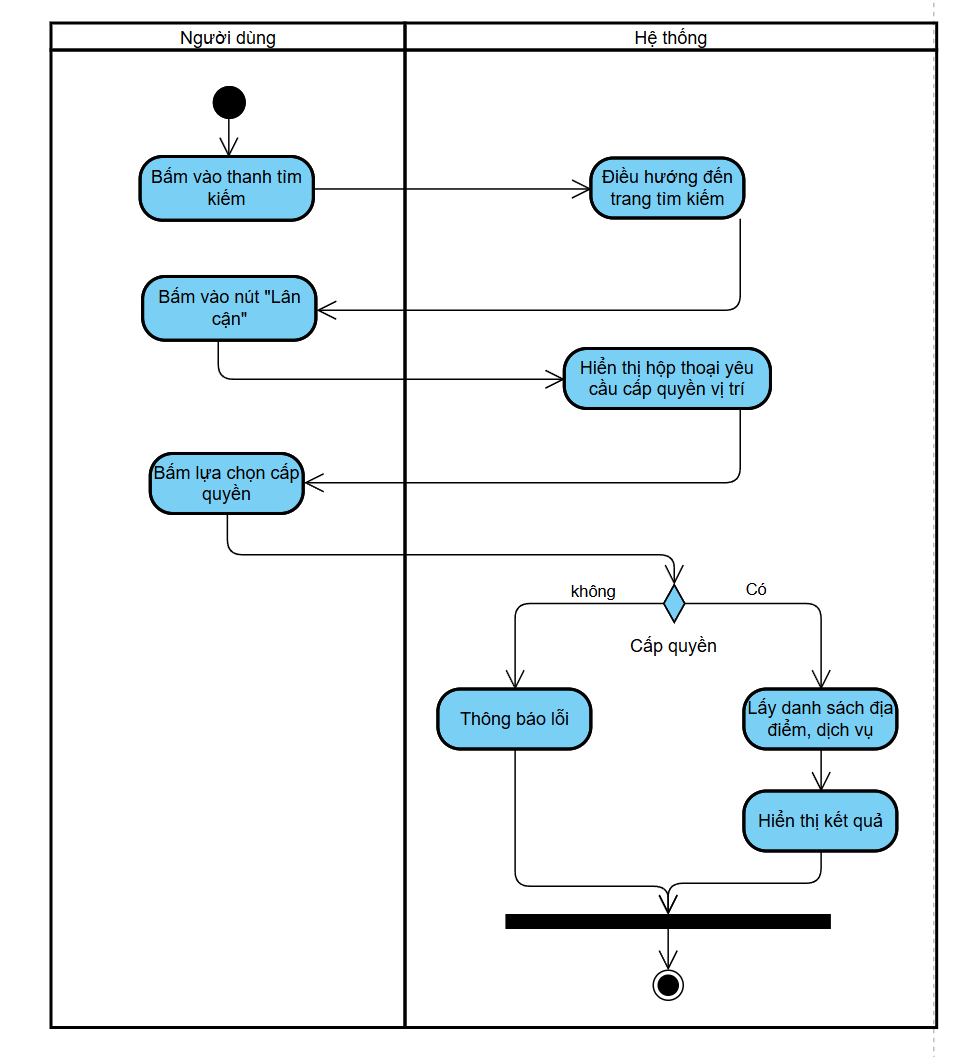
\includegraphics[width=0.5\linewidth]{figures/c3/3-3-7-ad.png} % Specified width
        &
        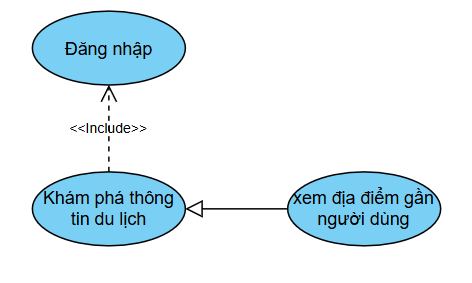
\includegraphics[width=0.45\linewidth]{figures/c3/3-3-7-rd.png} \\ % Specified width
        \hline
    \end{tabular}
\end{table}

\begin{figure}[H]
    \centering
    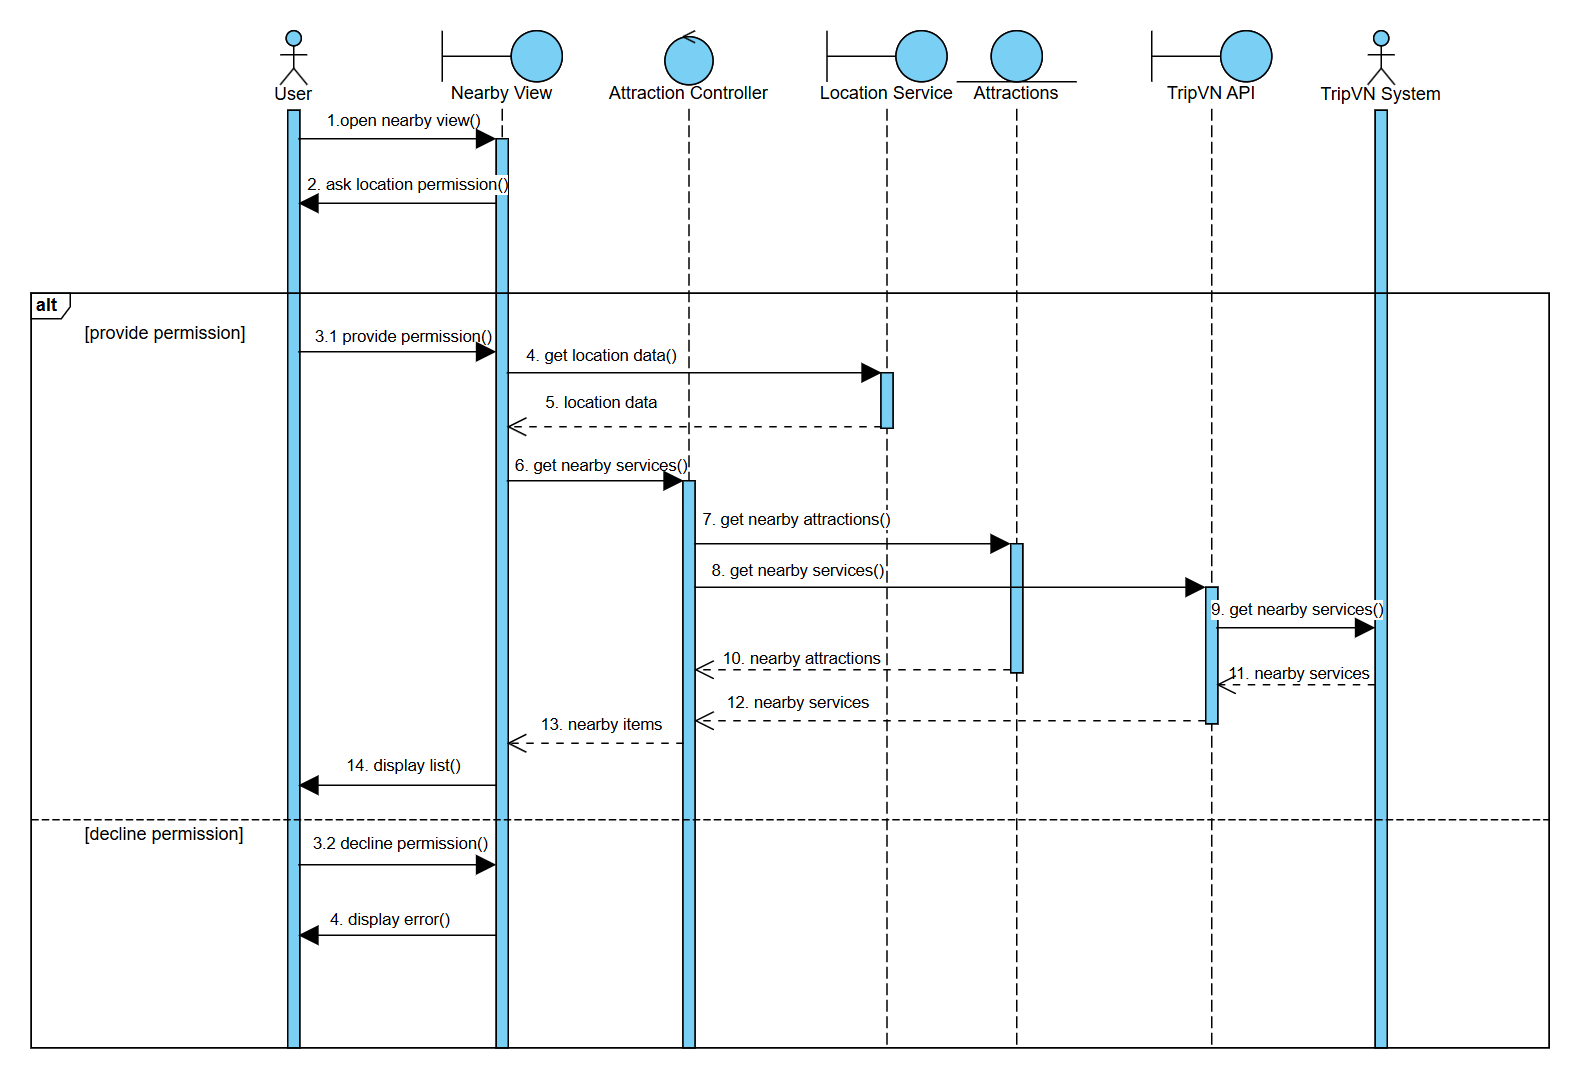
\includegraphics[width=1\textwidth]{figures/c3/3-3-7-sd.png} % Specified width
    \caption{Biểu đồ tuần tự ca sử dụng xem danh sách địa điểm gần người dùng.}
    \label{fig:3-3-7-sequence-diagram}
\end{figure}
\nopagebreak
\subsection{Ca sử dụng xem thông tin chi tiết địa điểm du lịch}
\noindent Ca sử dụng này mô tả cách người dùng xem thông tin chi tiết về một địa điểm du lịch cụ thể, bao gồm mô tả, hình ảnh, địa chỉ, đánh giá và các địa điểm liên quan khác. Bảng~\ref{tab:uc_view_place_details_spec} trình bày chi tiết đặc tả ca sử dụng, bao gồm luồng sự kiện chính, các điều kiện và yêu cầu liên quan. Các biểu đồ hoạt động, quan hệ (Bảng~\ref{tab:uc_view_place_details_diagrams}) và tuần tự (Hình~\ref{fig:3-3-8-sequence-diagram}) minh họa rõ hơn về quy trình và tương tác hệ thống khi người dùng xem chi tiết địa điểm.
% \vspace{0.5cm} % Adjust spacing if needed

% Use longtable environment
% Need \usepackage{longtable} and \usepackage{calc} in preamble
\begin{longtable}{| p{4cm} | p{\dimexpr\linewidth-4cm-4\tabcolsep} |} % Adjust widths as needed
    \caption{Đặc tả ca sử dụng xem thông tin chi tiết địa điểm du lịch} % Caption inside longtable
    \label{tab:uc_view_place_details_spec} \\ % Label after caption

    \hline
    \textbf{Mô tả} & Người dùng xem chi tiết thông tin địa điểm du lịch. \\
    \hline
    \endfirsthead % Header for the first page

    % No \endhead content needed

    % No \endfoot content needed

    \hline % Footer for the last page
    \endlastfoot

    % --- Table Content ---
    \textbf{Luồng cơ bản} & 1. Người dùng bấm vào một địa điểm du lịch muốn xem thông tin (từ danh sách tìm kiếm, gợi ý, bản đồ, v.v.). \newline
                           2. Hệ thống lấy thông tin chi tiết của địa điểm từ cơ sở dữ liệu và các API bên ngoài (nếu cần). \newline
                           3. Hệ thống hiển thị thông tin chi tiết địa điểm du lịch bao gồm tên, mô tả, địa chỉ, số điện thoại, ảnh, đánh giá và các địa điểm liên quan. \\
    \hline
    % \textbf{Luồng thay thế} & (Nếu có luồng thay thế, ví dụ: địa điểm không tồn tại, lỗi API) \\
    % \hline
    \textbf{Tiền điều kiện} & Người dùng đang đăng nhập và phiên đăng nhập chưa kết thúc. \\
    \hline
    \textbf{Hậu điều kiện} & - Người dùng có thể xem thông tin về địa điểm như mô tả, địa chỉ, sđt, ảnh. \newline
                           - Người dùng có thể xem chi tiết các đánh giá về địa điểm. \newline
                           - Người dùng có thể xem chi tiết các địa điểm liên quan. \\
    \hline
    \textbf{Yêu cầu phi chức năng} & Hệ thống xử lý lấy và hiển thị thông tin không quá 2 giây. \\
    % --- End Table Content ---

\end{longtable}
\vspace{0.8cm}

\begin{table}[H] % Wrap the diagrams table
    \centering
    \caption{Biểu đồ hoạt động ca sử dụng xem thông tin chi tiết địa điểm du lịch} % Add caption
    \label{tab:uc_view_place_details_diagrams} % Add label
    \begin{tabular}{| c | c |}
        \hline
        \textbf{Biểu đồ hoạt động} & \textbf{Quan hệ} \\
        \hline
        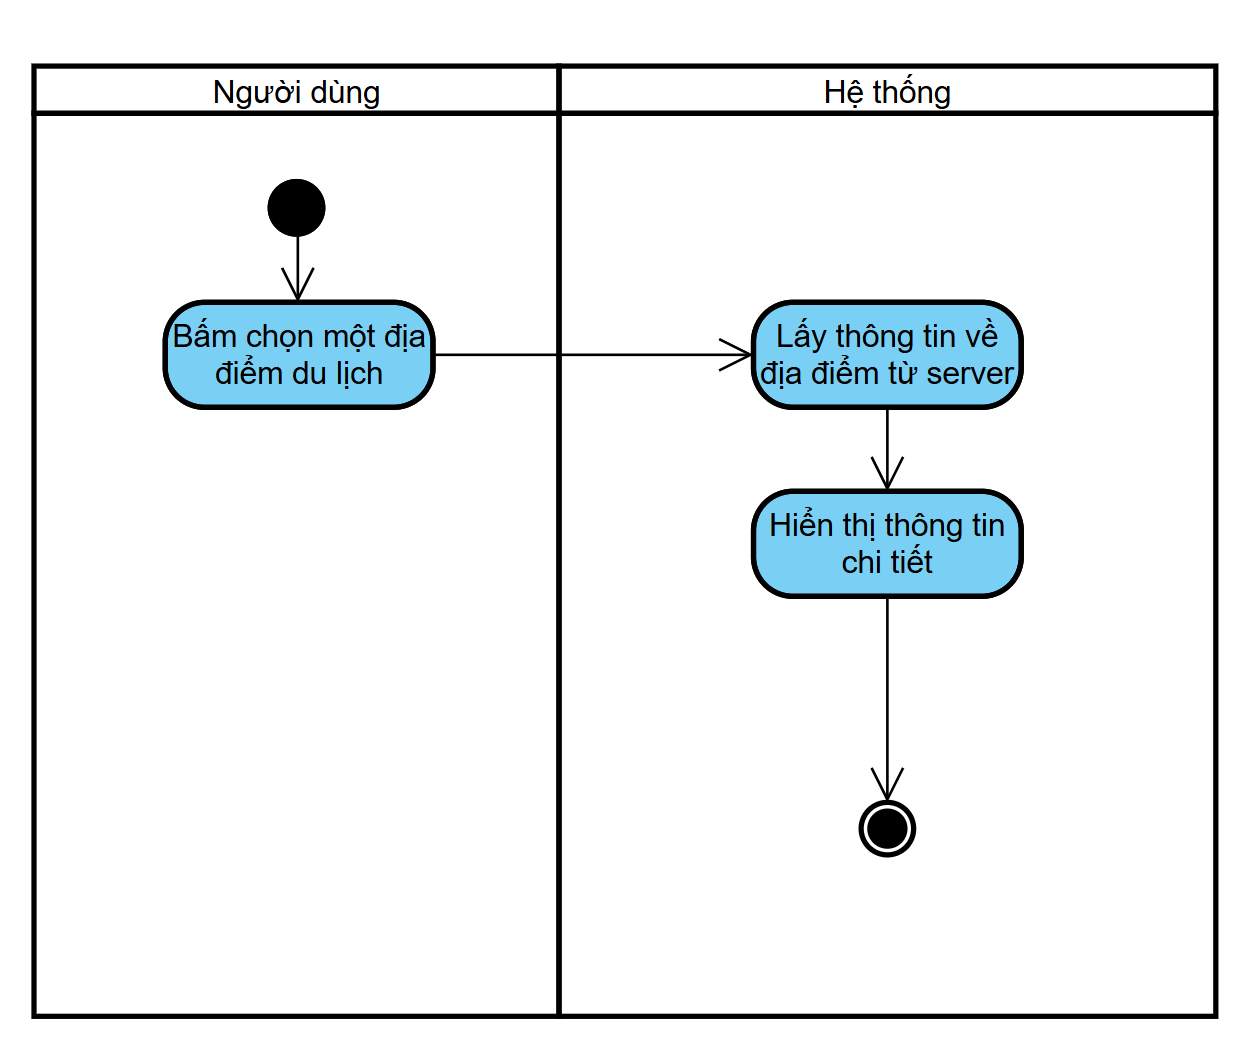
\includegraphics[width=0.5\linewidth]{figures/c3/3-3-8-ad.png} % Specified width
        &
        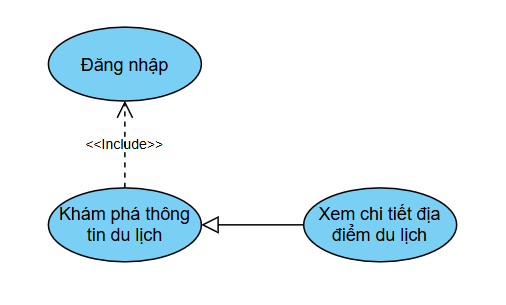
\includegraphics[width=0.45\linewidth]{figures/c3/3-3-8-rd.png} \\ % Specified width
        \hline
    \end{tabular}
\end{table}

\begin{figure}[H]
    \centering
    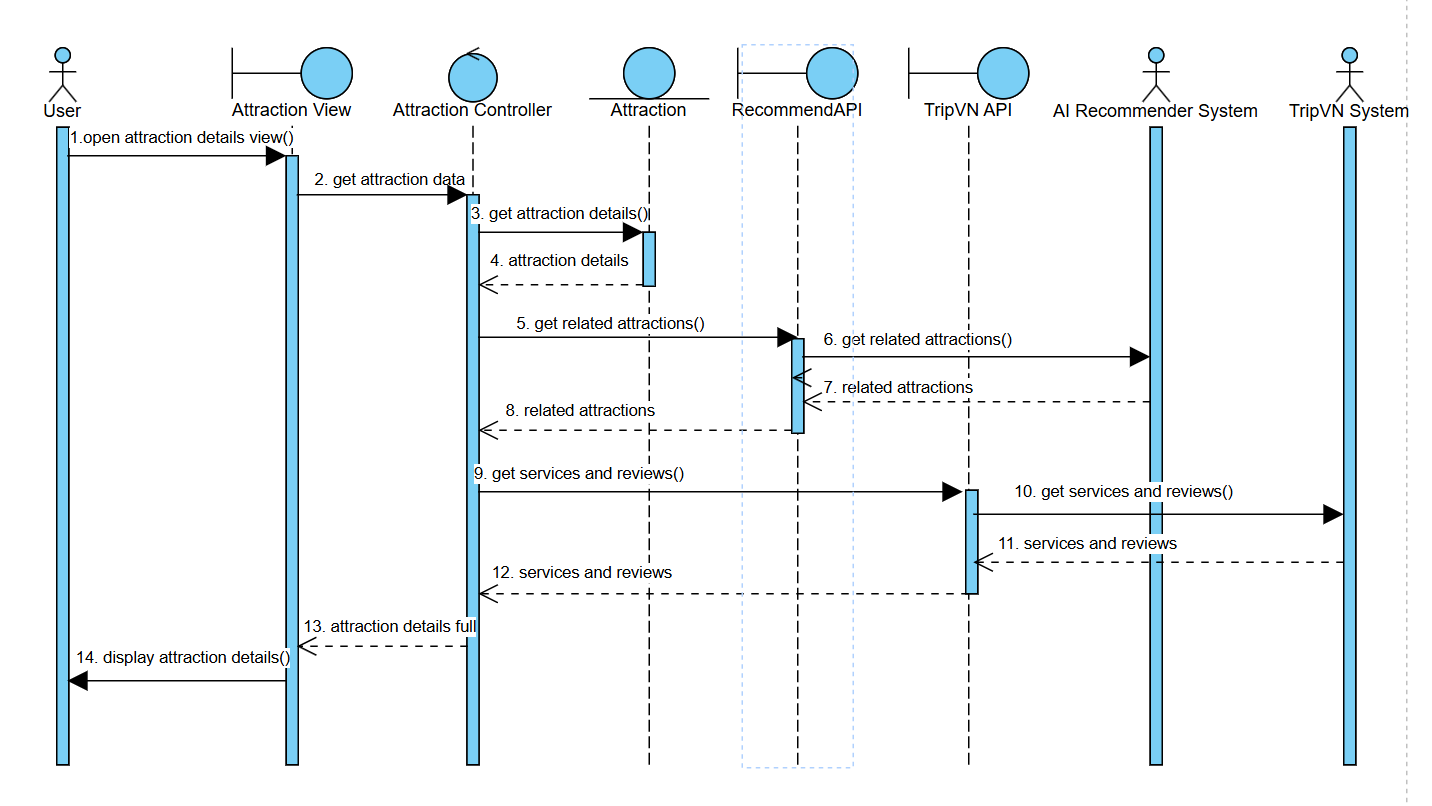
\includegraphics[width=1\textwidth]{figures/c3/3-3-8-sd.png} % Specified width
    \caption{Biểu đồ tuần tự ca sử dụng xem thông tin chi tiết địa điểm du lịch.}
    \label{fig:3-3-8-sequence-diagram}
\end{figure}
\nopagebreak
\subsection{Ca sử dụng gửi tin nhắn}
\vspace{0.5cm}


\noindent 
\begin{tabularx}{\linewidth}{| l | X |} 
\hline 
\textbf{Mô tả} & Người dùng có thể gửi tin nhắn trong nhóm hoặc gửi tin nhắn riêng cho bạn bè.  \\ 
\hline 
\textbf{Luồng cơ bản} & 1. Người dùng truy cập tab tin nhắn. \newline
                        2. Người dùng bấm vào một cuộc hội thoại muốn gửi tin nhắn. \newline
                        3. Hệ thống hiển thị thông tin của cuộc hội thoại và các tin nhắn trong cuộc hội thoại đó. \newline
                        4. Người dùng nhập tin nhắn muốn gửi. \newline
                        5. Người dùng bấm gửi. \newline
                        6. Hệ thống gửi tin nhắn và hiển thị tin nhắn vừa gửi lên cuộc hội thoại. \\
                        
\hline 
\textbf{Luồng thay thế} & Người dùng đính kèm địa điểm vào tin nhắn \newline
   1. Người dùng nhấn nút "+" cạnh ô input. \newline
   2. Hệ thống hiển thị giao diện tìm kiếm/chọn địa điểm. \newline
   3. Người dùng chọn một địa điểm. \newline
   4. Hệ thống thêm thông tin địa điểm đã chọn vào nội dung tin nhắn đang soạn thảo. \\

                       
\hline 
\textbf{Tiền điều kiện} &- Người dùng đang đăng nhập và phiên đăng nhập chưa kết thúc. \newline
                        - Người dùng đã có ít nhất một cuộc hội thoại. \\
\hline 
\textbf{Hậu điều kiện} & - Hệ thống lưu tin nhắn vào cơ sở dữ liệu và hiển thị tin nhắn trong cuộc hội thoại trong thời gian thực. \newline
                        - Hệ thống nhận diện địa điểm trong tin nhắn và highlight các địa điểm đó. \newline
                        - Hệ thống phân loại tin nhắn có cần thiết cho tổng hợp lịch trìn hay không. \newline
                        - Người dùng có thể nhấn vào địa điểm trong tin nhắn để xem chi tiết địa điểm. \newline
                        - Người dùng có thể react hoặc gỡ tin nhắn\\

\hline 
\textbf{Yêu cầu phi chức năng} & Hệ thống xử lý gửi tin nhắn dưới 1s  \\ 
\hline 
\end{tabularx}



\noindent 
\begin{tabular}{| c | c |}
    \hline
    \textbf{Biểu đồ hoạt động} & \textbf{Quan hệ} \\ 
    \hline
    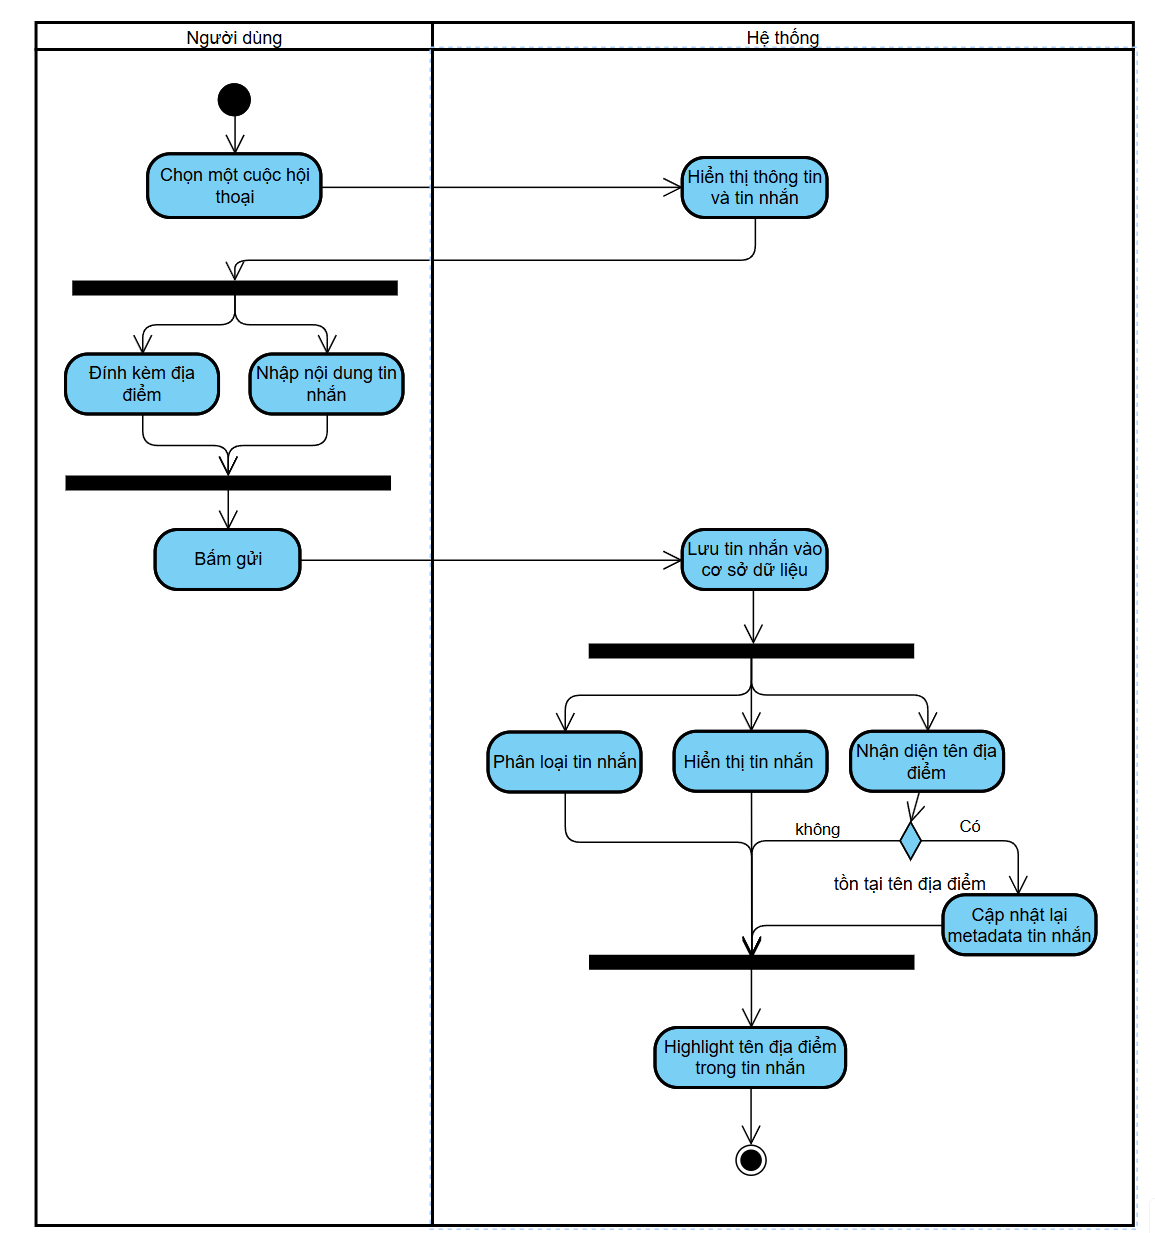
\includegraphics[width=0.5\linewidth]{figures/c3/3-3-9-ad.png} 
    & 
    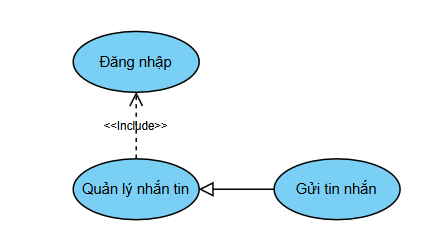
\includegraphics[width=0.45\linewidth]{figures/c3/3-3-9-rd.png} \\ 
    \hline
\end{tabular}


\vspace{0.8cm}

\begin{figure}[H]
    \centering  
    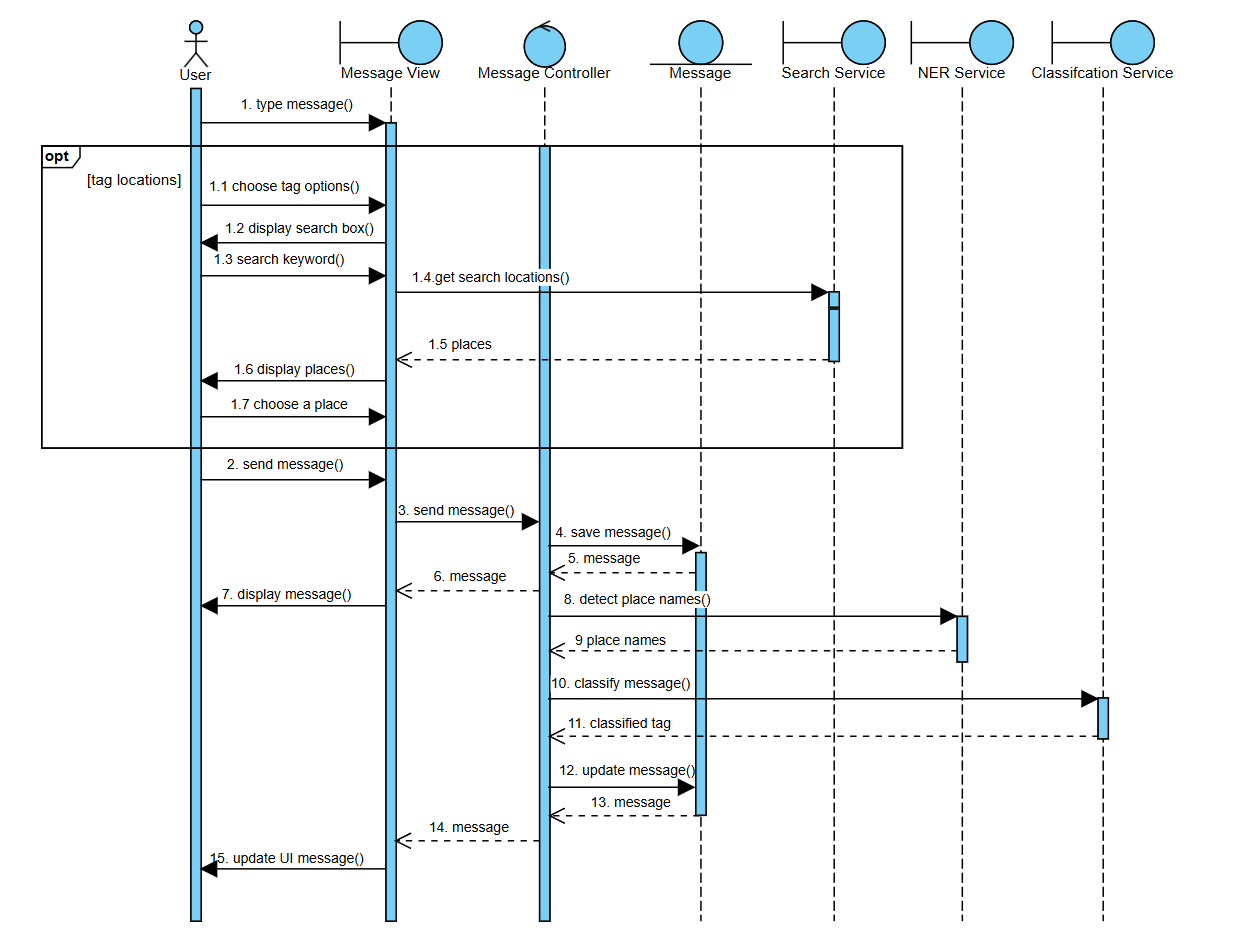
\includegraphics[width=1\textwidth]{figures/c3/3-3-9-sd.png}
    \caption{Biểu đồ tuần tự ca sử dụng gửi tin nhắn.}
    \label{fig:3-3-9-sequence-diagram}
\end{figure}
\nopagebreak
\subsection{Ca sử dụng tổng hợp lịch trình từ hội thoại}
\vspace{0.5cm}


\noindent 
\begin{tabularx}{\linewidth}{| l | X |} 
\hline 
\textbf{Mô tả} & Hệ thống sẽ tổng hợp lại lịch trình được đúc kết từ đoạn tin nhắn trong nhóm chat của người dùng.  \\ 
\hline 
\textbf{Luồng cơ bản} & 1. Người dùng bấm vào một cuộc hội thoại nhóm muốn tổng hợp. \newline
                        2. Hệ thống hiển thị thông cuộc hội thoại và các tin nhắn trong cuộc hội thoại đó. \newline
                        3. Người dùng chọn tùy chọn tổng hợp tin nhắn. \newline
                        4. Hệ thống lấy và hiển thị lịch trình tổng hợp của cuộc hội thoại (nếu có) . \newline
                        5. Người dùng bấm "Tổng hợp". \newline
                        6. Hệ thống sử dụng AI tổng hợp lịch trình trong cuộc hội thoại và hiển thị lịch trình tổng hợp. \\
                        
\hline 
\textbf{Luồng thay thế} & Hệ thống thông báo lỗi khi không có tin nhắn mới chưa được cập nhật. \\

                       
\hline 
\textbf{Tiền điều kiện} &- Người dùng đang đăng nhập và phiên đăng nhập chưa kết thúc. \newline
                        - Người dùng đã có ít nhất một cuộc hội thoại nhóm. \\
\hline 
\textbf{Hậu điều kiện} & - Hệ thống tổng hợp lịch trình sau đó lưu vào cơ sở dữ liệu và hiển thị cho người dùng. \newline
                        - Hệ thống đánh dấu các tin nhắn đã được tổng hợp. \newline
                        - Hệ thống gộp lịch trình với lịch trình đã tổng hợp trước đó.\\

\hline 
\textbf{Yêu cầu phi chức năng} & Hệ thống xử lý tổng hợp lịch trình dưới 10s  \\ 
\hline 
\end{tabularx}



\noindent 
\begin{tabular}{| c | c |}
    \hline
    \textbf{Biểu đồ hoạt động} & \textbf{Quan hệ} \\ 
    \hline
    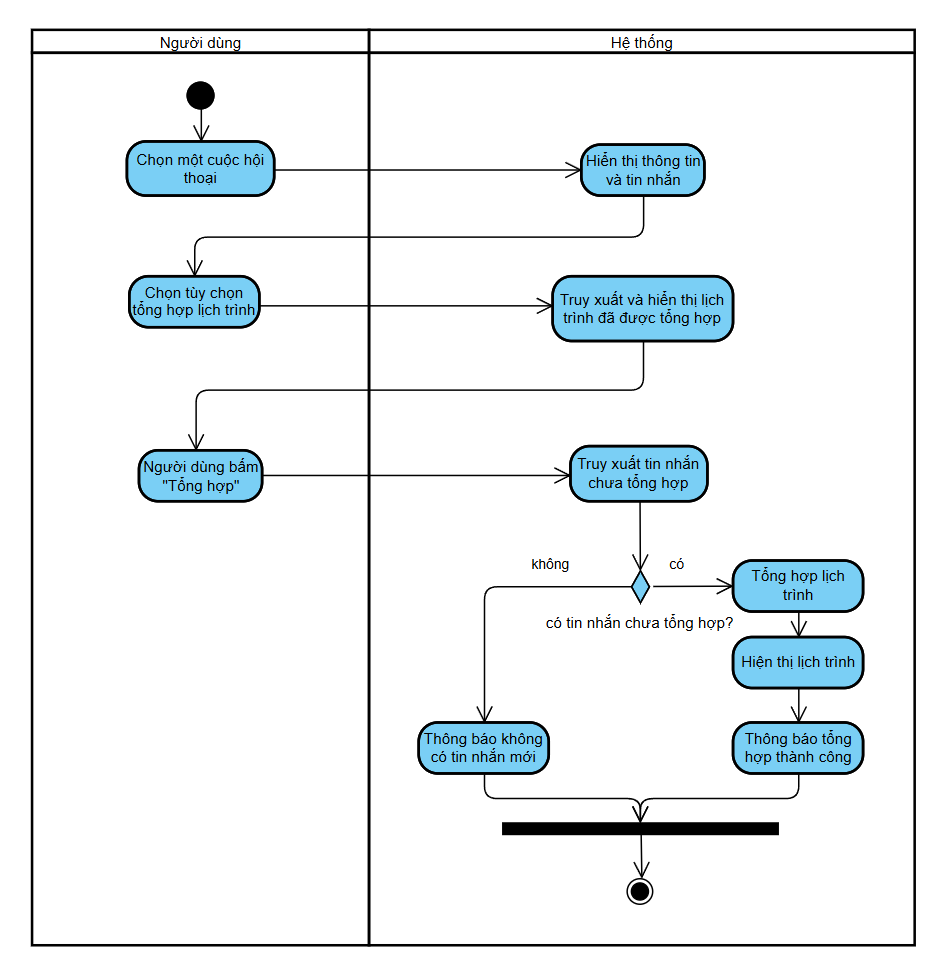
\includegraphics[width=0.5\linewidth]{figures/c3/3-3-10-ad.png} 
    & 
    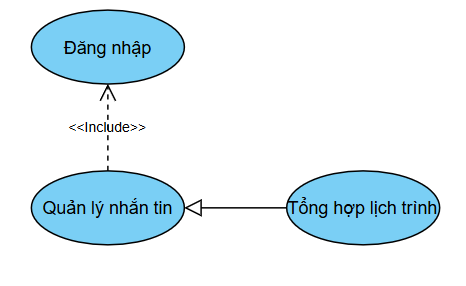
\includegraphics[width=0.45\linewidth]{figures/c3/3-3-10-rd.png} \\ 
    \hline
\end{tabular}


\vspace{0.8cm}

\begin{figure}[H]
    \centering  
    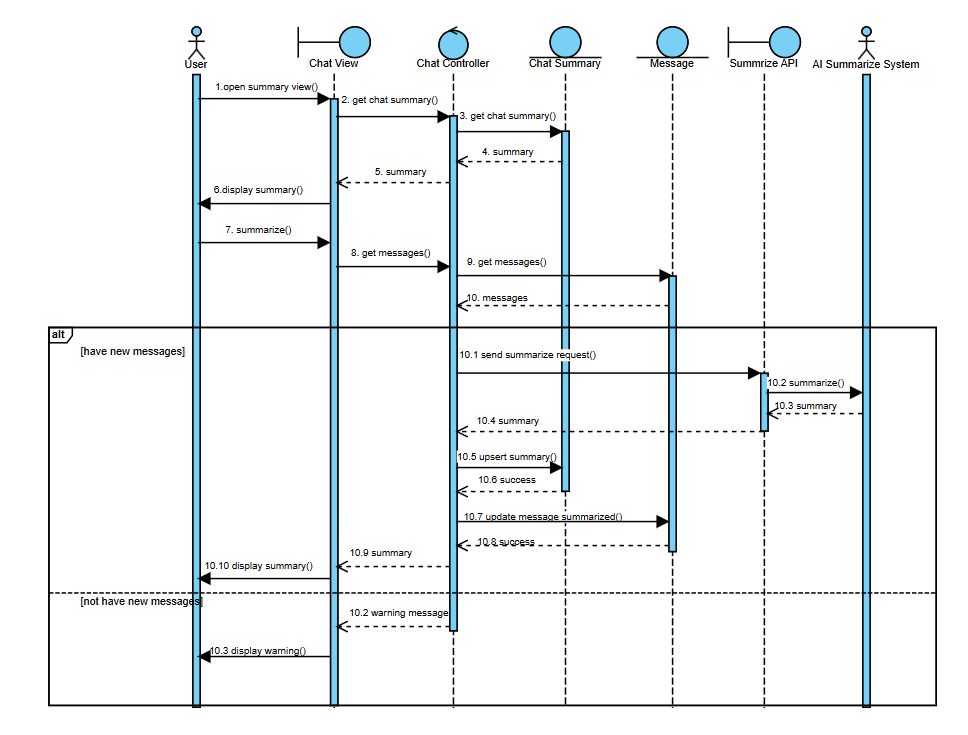
\includegraphics[width=1\textwidth]{figures/c3/3-3-10-sd.png}
    \caption{Biểu đồ tuần tự ca sử dụng tổng hợp lịch trình.}
    \label{fig:3-3-10-sequence-diagram}
\end{figure}
\nopagebreak
\subsection{Ca sử dụng tạo chuyến đi mặc định}
\noindent Ca sử dụng này mô tả cách người dùng tạo nhanh một chuyến đi mới chỉ với tên chuyến đi. Chuyến đi này mặc định sẽ ở chế độ riêng tư và người dùng có thể cập nhật chi tiết sau. Bảng~\ref{tab:uc_create_default_trip_spec} trình bày chi tiết đặc tả ca sử dụng, bao gồm luồng sự kiện chính, luồng thay thế, các điều kiện và yêu cầu liên quan. Các biểu đồ hoạt động, quan hệ (Bảng~\ref{tab:uc_create_default_trip_diagrams}) và tuần tự (Hình~\ref{fig:3-3-11-sequence-diagram}) minh họa rõ hơn về quy trình và tương tác hệ thống.
% \vspace{0.5cm} % Adjust spacing if needed

% Use longtable environment
% Need \usepackage{longtable} and \usepackage{calc} in preamble
\begin{longtable}{| p{4cm} | p{\dimexpr\linewidth-4cm-4\tabcolsep} |} % Adjust widths as needed
    \caption{Đặc tả ca sử dụng tạo chuyến đi mặc định} % Caption inside longtable
    \label{tab:uc_create_default_trip_spec} \\ % Label after caption

    \hline
    \textbf{Mô tả} & Người dùng có thể tạo chuyến đi để lên kế hoạch du lịch cho bản thân và bạn bè. \\
    \hline
    \endfirsthead % Header for the first page

    % No \endhead content needed

    % No \endfoot content needed

    \hline % Footer for the last page
    \endlastfoot

    % --- Table Content ---
    \textbf{Luồng cơ bản} & 1. Người dùng bấm vào tab chuyến đi. \newline
                           2. Người dùng bấm vào dấu ``+'' góc phải trên. \newline
                           3. Hệ thống hiển thị hộp thoại yêu cầu người dùng nhập tên cho chuyến đi. \newline
                           4. Người dùng nhập tên chuyến đi. \newline
                           5. Người dùng bấm ``Tạo". \newline
                           6. Hệ thống tạo một chuyến đi mới với tên đã đặt. \\
    \hline
    \textbf{Luồng thay thế} & Hệ thống thông báo lỗi khi tên chuyến đi dài hơn 80 kí tự. \\
    \hline
    \textbf{Tiền điều kiện} & - Người dùng đang đăng nhập và phiên đăng nhập chưa kết thúc. \\
    \hline
    \textbf{Hậu điều kiện} & - Hệ thống thêm chuyến đi với trạng thái là riêng tư của người dùng vào cơ sở dữ liệu. \\
    \hline
    \textbf{Yêu cầu phi chức năng} & Hệ thống tạo chuyến đi dưới 2s. \\
    % --- End Table Content ---

\end{longtable}


\begin{table}[H] % Wrap the diagrams table
    \centering
    \caption{Biểu đồ hoạt động và quan hệ ca sử dụng tạo chuyến đi mặc định} % Add caption
    \label{tab:uc_create_default_trip_diagrams} % Add label
    \begin{tabular}{| c | c |}
        \hline
        \textbf{Biểu đồ hoạt động} & \textbf{Quan hệ} \\
        \hline
        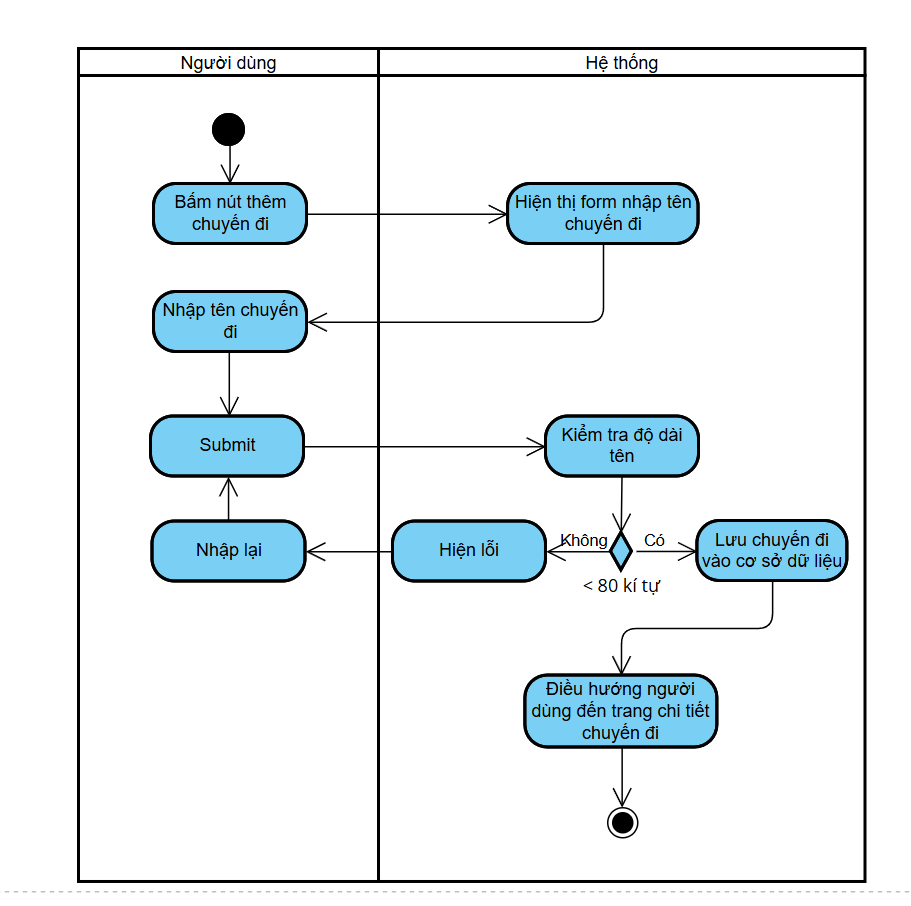
\includegraphics[width=0.5\linewidth]{figures/c3/3-3-11-ad.png} % Specified width
        &
        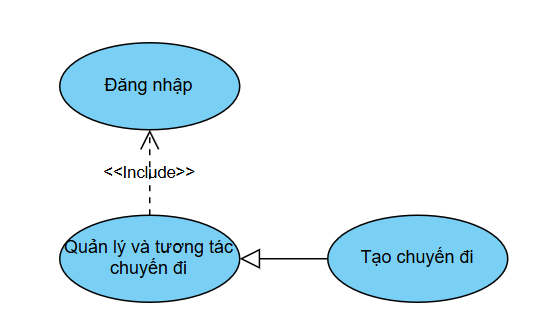
\includegraphics[width=0.45\linewidth]{figures/c3/3-3-11-rd.png} \\ % Specified width
        \hline
    \end{tabular}
\end{table}

\begin{figure}[H]
    \centering
    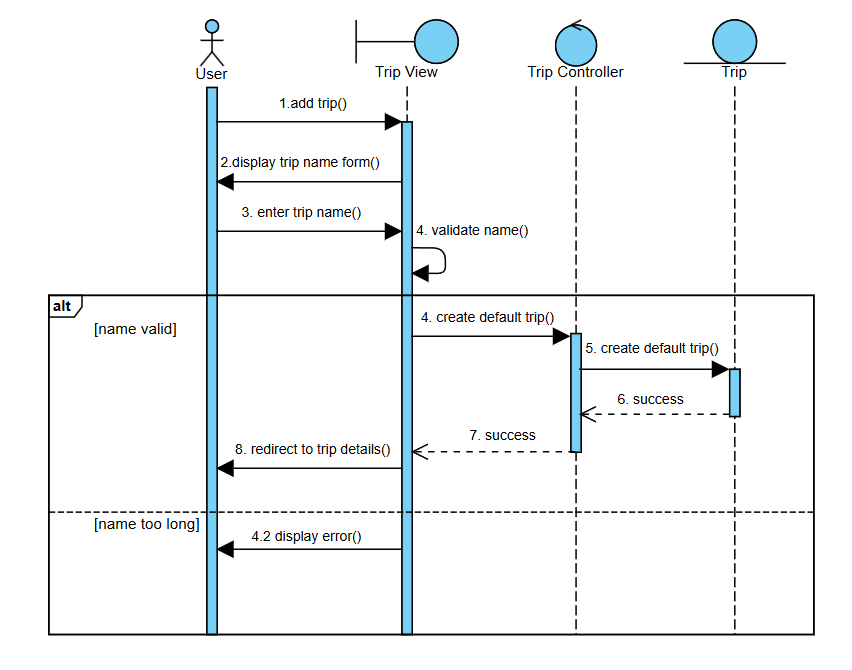
\includegraphics[width=0.95\textwidth]{figures/c3/3-3-11-sd.png} % Specified width
    \caption{Biểu đồ tuần tự ca sử dụng tạo chuyến đi mặc định.}
    \label{fig:3-3-11-sequence-diagram}
\end{figure}
\nopagebreak
\subsection{Ca sử dụng thêm mục lưu trữ vào chuyến đi}
\noindent Ca sử dụng này mô tả cách người dùng lưu các địa điểm, sự kiện, hoặc nhà hàng vào một chuyến đi cụ thể để tham khảo khi lên lịch trình. Người dùng có thể tìm kiếm và chọn các mục muốn lưu. Bảng~\ref{tab:uc_add_saved_item_spec} trình bày chi tiết đặc tả ca sử dụng, bao gồm luồng sự kiện chính, luồng thay thế, các điều kiện và yêu cầu liên quan. Các biểu đồ hoạt động, quan hệ (Bảng~\ref{tab:uc_add_saved_item_diagrams}) và tuần tự (Hình~\ref{fig:3-3-12-sequence-diagram}) minh họa rõ hơn về quy trình và tương tác hệ thống.
% \vspace{0.5cm} % Adjust spacing if needed

% Use longtable environment
% Need \usepackage{longtable} and \usepackage{calc} in preamble
\begin{longtable}{| p{4cm} | p{\dimexpr\linewidth-4cm-4\tabcolsep} |} % Adjust widths as needed
    \caption{Đặc tả ca sử dụng thêm mục lưu trữ vào chuyến đi} % Caption inside longtable (no period)
    \label{tab:uc_add_saved_item_spec} \\ % Label after caption

    \hline
    \textbf{Mô tả} & Người dùng có thể lưu các địa điểm, sự kiện, nhà hàng vào chuyến đi để lên lịch trình dựa trên nó. \\
    \hline
    \endfirsthead % Header for the first page

    % No \endhead content needed

    % No \endfoot content needed

    \hline % Footer for the last page
    \endlastfoot

    % --- Table Content ---
    \textbf{Luồng cơ bản} & 1. Người dùng chọn một chuyến đi muốn thêm mục lưu. \newline
                           2. Hệ thống lấy dữ liệu chi tiết của chuyến đi và hiển thị. \newline
                           3. Người dùng bấm ``Thêm mục lưu". \newline
                           4. Hệ thống điều hướng sang trang thêm mục lưu và hiển thị thanh tìm kiếm. \newline
                           5. Người dùng nhập tên địa điểm, sự kiện hoặc nhà hàng muốn thêm vào chuyến đi. \newline
                           6. Hệ thống tìm kiếm và hiển thị danh sách các mục lưu phù hợp với từ khóa tìm kiếm. \newline
                           7. Người dùng chọn mục muốn lưu trong danh sách. \newline
                           8. Hệ thống thông báo đã thêm thành công. \\
    \hline
    \textbf{Luồng thay thế} & Người dùng bấm vào mục đã lưu sẽ bỏ lưu mục đấy. \\
    \hline
    \textbf{Tiền điều kiện} & - Người dùng đang đăng nhập và phiên đăng nhập chưa kết thúc.\newline
                           - Người dùng đã tạo hoặc tham gia ít nhất một chuyến đi. \newline
                           - Trạng thái chuyến đi khác ``Đã hoàn thành'' và ``Hủy". \\
    \hline
    \textbf{Hậu điều kiện} & - Hệ thống thêm mục lưu của chuyến đi vào cơ sở dữ liệu.\newline
                           - Người dùng có thể xem lại mục lưu đã thêm vào chuyến đi. \\
    \hline
    \textbf{Yêu cầu phi chức năng} & Hệ thống thêm mục lưu dưới 1s. \\
    % --- End Table Content ---

\end{longtable}


\begin{table}[H] % Wrap the diagrams table
    \centering
    \caption{Biểu đồ hoạt động ca sử dụng thêm mục lưu trữ vào chuyến đi} % Add caption (no period)
    \label{tab:uc_add_saved_item_diagrams} % Add label
    \begin{tabular}{| c | c |}
        \hline
        \textbf{Biểu đồ hoạt động} & \textbf{Quan hệ} \\
        \hline
        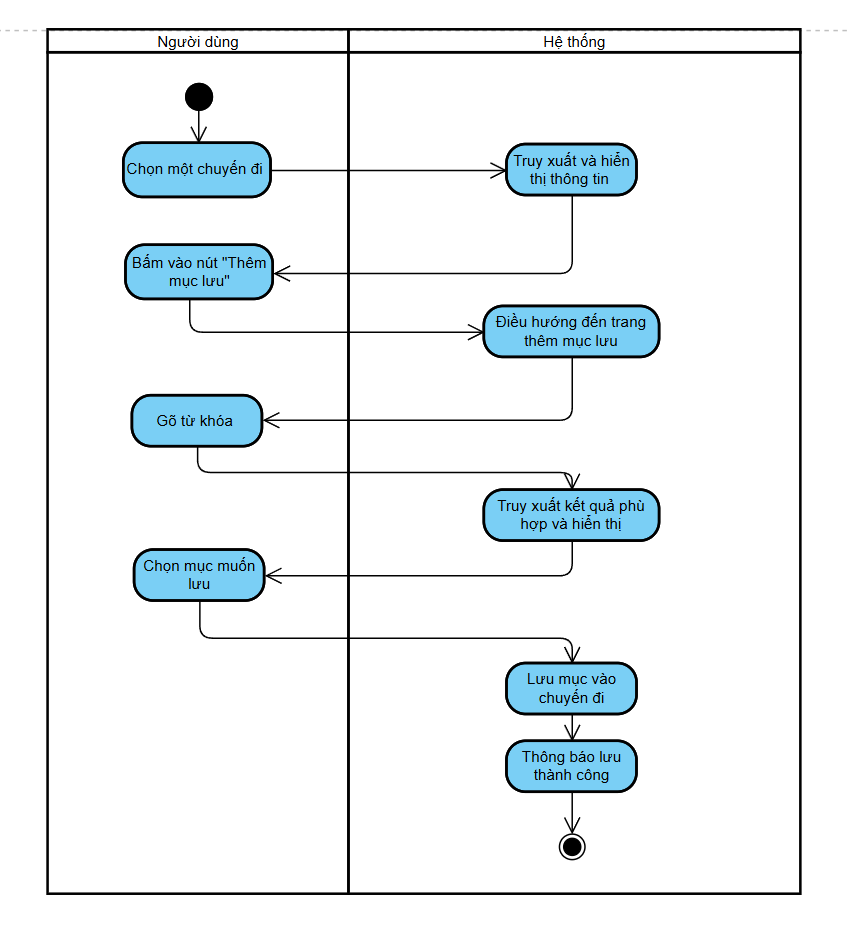
\includegraphics[width=0.5\linewidth]{figures/c3/3-3-12-ad.png} % Specified width
        &
        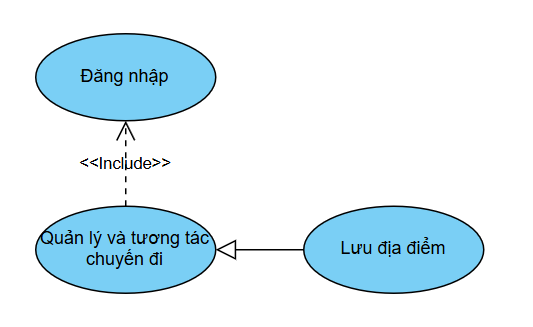
\includegraphics[width=0.45\linewidth]{figures/c3/3-3-12-rd.png} \\ % Specified width
        \hline
    \end{tabular}
\end{table}

\begin{figure}[H]
    \centering
    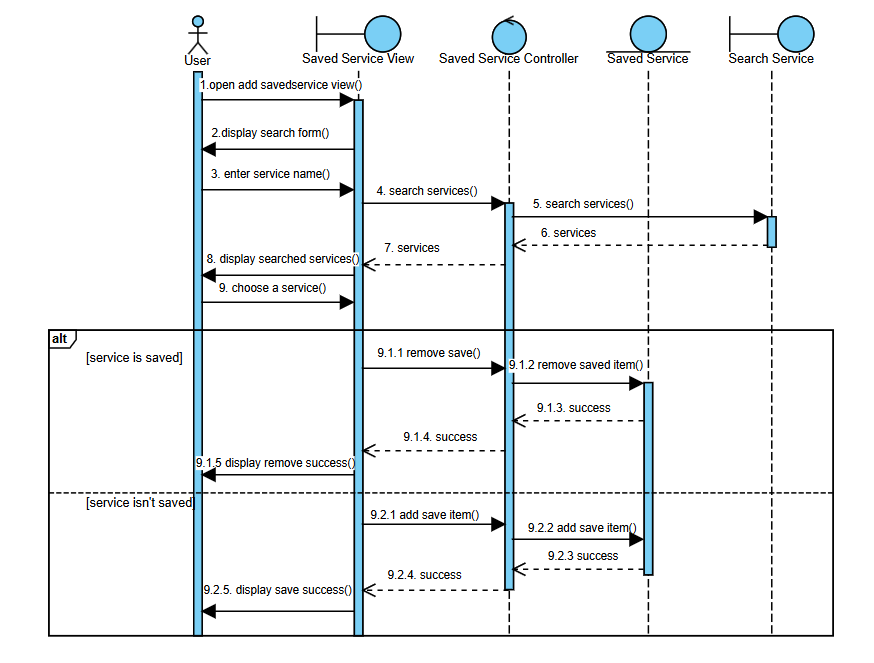
\includegraphics[width=0.92\textwidth]{figures/c3/3-3-12-sd.png} % Specified width
    \caption{Biểu đồ tuần tự ca sử dụng thêm mục lưu vào chuyến đi.} % (no period)
    \label{fig:3-3-12-sequence-diagram}
\end{figure}
\nopagebreak
\subsection{Ca sử dụng tạo lịch trình cho chuyến đi}
\noindent Ca sử dụng này mô tả cách người dùng tạo một mục lịch trình cụ thể cho một ngày trong chuyến đi của họ. Người dùng có thể chọn địa điểm từ danh sách đã lưu hoặc chọn trực tiếp trên bản đồ, sau đó cung cấp thông tin chi tiết như thời gian và ghi chú. Bảng~\ref{tab:uc_create_itinerary_item_spec} trình bày chi tiết đặc tả ca sử dụng, bao gồm luồng sự kiện chính, luồng thay thế, các điều kiện và yêu cầu liên quan. Các biểu đồ hoạt động, quan hệ (Bảng~\ref{tab:uc_create_itinerary_item_diagrams}) và tuần tự (Hình~\ref{fig:3-3-13-sequence-diagram}) minh họa rõ hơn về quy trình và tương tác hệ thống.
% \vspace{0.5cm} % Adjust spacing if needed

% Use longtable environment
% Need \usepackage{longtable} and \usepackage{calc} in preamble
\begin{longtable}{| p{4cm} | p{\dimexpr\linewidth-4cm-4\tabcolsep} |} % Adjust widths as needed
    \caption{Đặc tả ca sử dụng tạo lịch trình cho chuyến đi} % Caption inside longtable (no period)
    \label{tab:uc_create_itinerary_item_spec} \\ % Label after caption

    \hline
    \textbf{Mô tả} & Người dùng có thể tạo một lịch trình cụ thể cho chuyến đi của mình. \\
    \hline
    \endfirsthead % Header for the first page

    % No \endhead content needed

    % No \endfoot content needed

    \hline % Footer for the last page
    \endlastfoot

    % --- Table Content ---
    \textbf{Luồng cơ bản} & 1. Người dùng chọn một chuyến đi. \newline
                           2. Hệ thống lấy dữ liệu chi tiết và hiển thị. \newline
                           3. Người dùng bấm ``Thêm lịch trình". \newline
                           4. Hệ thống hiển thị 2 lựa chọn tạo lịch trình. \newline
                           5. Người dùng chọn tùy chọn ``chọn từ mục lưu". \newline
                           6. Hệ thống truy xuất và hiển thị các mục lưu của chuyến đi cho người dùng chọn. \newline
                           7. Người dùng chọn mục thêm vào lịch trình. \newline
                           8. Hệ thống hiển thị form điền thông tin lịch trình. \newline
                           9. Người dùng điền thông tin lịch trình như thời gian bắt đầu, ghi chú,v.v. \newline
                           10. Người dùng bấm ``Lưu lịch trình". \newline
                           11. Hệ thống lưu lịch trình vào cơ sở dữ liệu và thông báo thành công. \\
    \hline
    \textbf{Luồng thay thế} & \textbf{Chọn trên bản đồ:} \newline
                               1. Người dùng chọn tùy chọn ``chọn trên bản đồ". \newline
                               2. Hệ thống hiển thị bản đồ. \newline
                               3. Người dùng chọn 1 vị trí trên bản đồ. \newline
                               4. Tiếp tục từ bước 8 của Luồng cơ bản. \\
    \hline
    \textbf{Tiền điều kiện} & - Người dùng đang đăng nhập và phiên đăng nhập chưa kết thúc.\newline
                           - Người dùng đã tạo hoặc tham gia ít nhất một chuyến đi. \newline
                           - Trạng thái chuyến đi khác ``Đã hoàn thành'' và ``Hủy". \\
    \hline
    \textbf{Hậu điều kiện} & - Hệ thống lưu lịch trình vào cơ sở dữ liệu.\newline
                           - Người dùng có thể chỉnh sửa lịch trình đã tạo. \newline
                           - Người dùng có thể xem bản đồ trực quan lịch trình đã tạo. \\
    \hline
    \textbf{Yêu cầu phi chức năng} & Hệ thống thêm mục lưu dưới 2s \\
    % --- End Table Content ---

\end{longtable}
\vspace{0.8cm}

\begin{table}[H] % Wrap the diagrams table
    \centering
    \caption{Biểu đồ hoạt động và quan hệ ca sử dụng tạo lịch trình cho chuyến đi} % Add caption (no period)
    \label{tab:uc_create_itinerary_item_diagrams} % Add label
    \begin{tabular}{| c | c |}
        \hline
        \textbf{Biểu đồ hoạt động} & \textbf{Quan hệ} \\
        \hline
        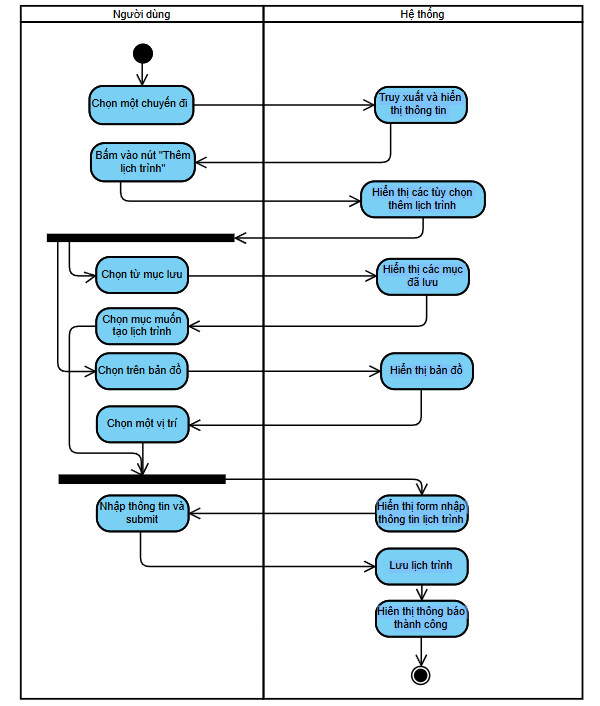
\includegraphics[width=0.5\linewidth]{figures/c3/3-3-13-ad.png} % Specified width
        &
        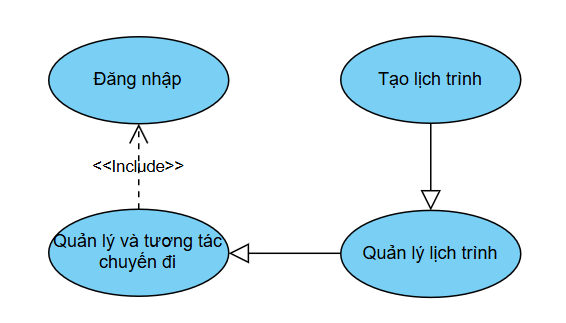
\includegraphics[width=0.45\linewidth]{figures/c3/3-3-13-rd.png} \\ % Specified width
        \hline
    \end{tabular}
\end{table}

\begin{figure}[H]
    \centering
    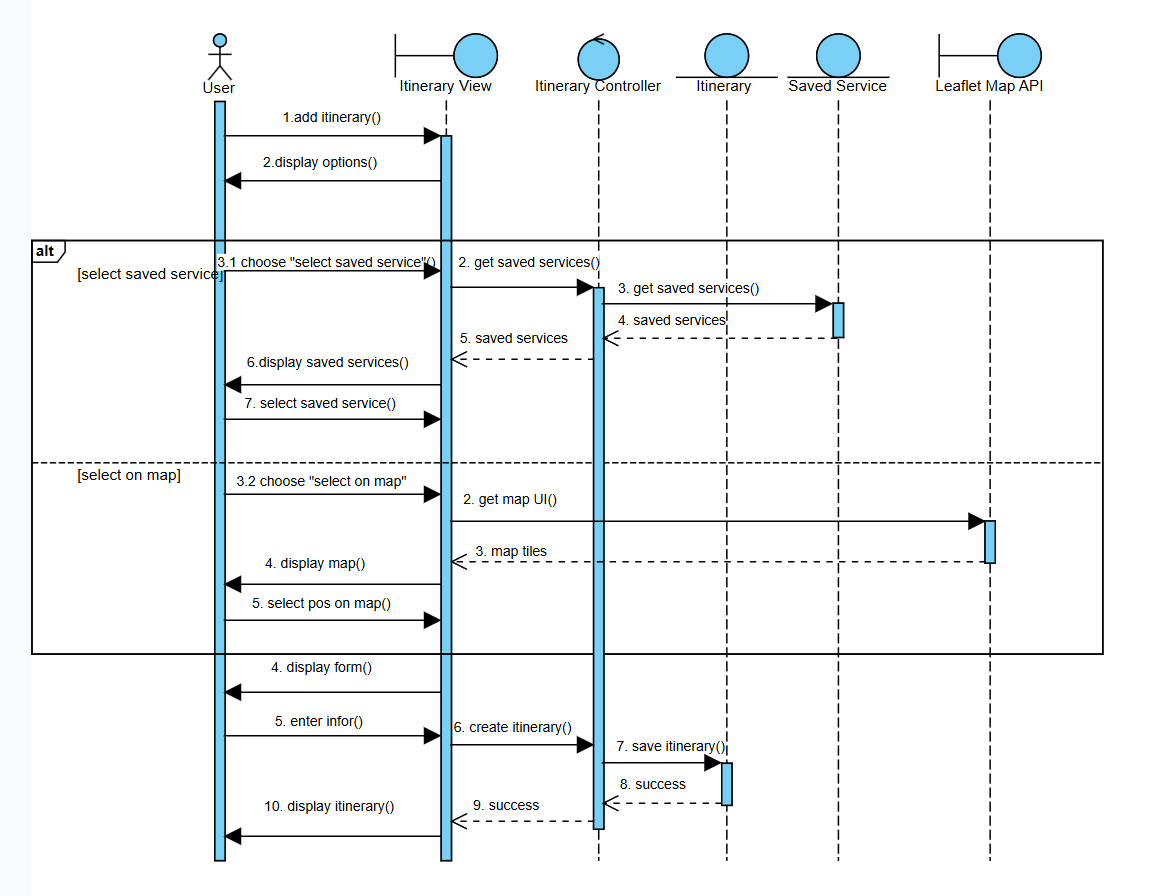
\includegraphics[width=1\textwidth]{figures/c3/3-3-13-sd.png} % Specified width
    \caption{Biểu đồ tuần tự ca sử dụng tạo lịch trình cho chuyến đi.} % (no period)
    \label{fig:3-3-13-sequence-diagram}
\end{figure}
\nopagebreak
% \subsection{Ca sử dụng mời bạn bè tham gia chuyến đi}
\noindent Ca sử dụng này mô tả cách người dùng mời bạn bè của họ tham gia vào một chuyến đi công khai mà họ đã tạo hoặc đang tham gia. Hệ thống sẽ gửi thông báo mời đến những người được chọn. Bảng~\ref{tab:uc_invite_friend_spec} trình bày chi tiết đặc tả ca sử dụng, bao gồm luồng sự kiện chính, luồng thay thế, các điều kiện và yêu cầu liên quan. Các biểu đồ hoạt động, quan hệ (Bảng~\ref{tab:uc_invite_friend_diagrams}) và tuần tự (Hình~\ref{fig:3-3-14-sequence-diagram}) minh họa rõ hơn về quy trình và tương tác hệ thống khi mời bạn bè.
% \vspace{0.5cm} % Adjust spacing if needed

% Use longtable environment
% Need \usepackage{longtable} and \usepackage{calc} in preamble
\begin{longtable}{| p{4cm} | p{\dimexpr\linewidth-4cm-4\tabcolsep} |} % Adjust widths as needed
    \caption{Đặc tả ca sử dụng mời bạn bè tham gia chuyến đi} % Caption inside longtable (no period)
    \label{tab:uc_invite_friend_spec} \\ % Label after caption

    \hline
    \textbf{Mô tả} & Người dùng có thể mời bạn bè tham gia chuyến đi của mình hoặc mình tham gia. \\
    \hline
    \endfirsthead % Header for the first page

    % No \endhead content needed

    % No \endfoot content needed

    \hline % Footer for the last page
    \endlastfoot

    % --- Table Content ---
    \textbf{Luồng cơ bản} & 1. Người dùng chọn một chuyến đi muốn mời bạn bè. \newline
                           2. Hệ thống lấy dữ liệu chi tiết của chuyến đi và hiển thị. \newline
                           3. Người dùng bấm ``Mời thành viên". \newline
                           4. Hệ thống điều hướng sang trang thêm thành viên và hiển thị thanh tìm kiếm. \newline
                           5. Người dùng nhập tên thành viên muốn mời. \newline
                           6. Hệ thống tìm kiếm và hiển thị danh sách các tài khoản phù hợp với từ khóa tìm kiếm. \newline
                           7. Người dùng chọn các tài khoản muốn mời. \newline
                           8. Hệ thống gửi thông báo mời vào chuyến đi và thông báo đã mời thành công. \\
    \hline
    \textbf{Luồng thay thế} & Người dùng được mời đã tham gia hoặc đã từ chối sẽ không được gửi thông báo tiếp. \\
    \hline
    \textbf{Tiền điều kiện} & - Người dùng đang đăng nhập và phiên đăng nhập chưa kết thúc.\newline
                           - Người dùng đã tạo hoặc tham gia ít nhất một chuyến đi. \newline
                           - Chuyến đi phải là chuyến đi công khai.\newline
                           - Trạng thái chuyến đi khác ``Đã hoàn thành'' và ``Hủy". \\
    \hline
    \textbf{Hậu điều kiện} & - Hệ thống gửi thông báo mời vào chuyến đi cho các tài khoản được chọn. \\
    \hline
    \textbf{Yêu cầu phi chức năng} & Hệ thống gửi lời mời bạn bè dưới 1s với 1 tài khoản. \\
    % --- End Table Content ---

\end{longtable}
\vspace{0.8cm}

\begin{table}[H] % Wrap the diagrams table
    \centering
    \caption{Biểu đồ hoạt động ca sử dụng mời bạn bè tham gia chuyến đi} % Add caption (no period)
    \label{tab:uc_invite_friend_diagrams} % Add label
    \begin{tabular}{| c | c |}
        \hline
        \textbf{Biểu đồ hoạt động} & \textbf{Quan hệ} \\
        \hline
        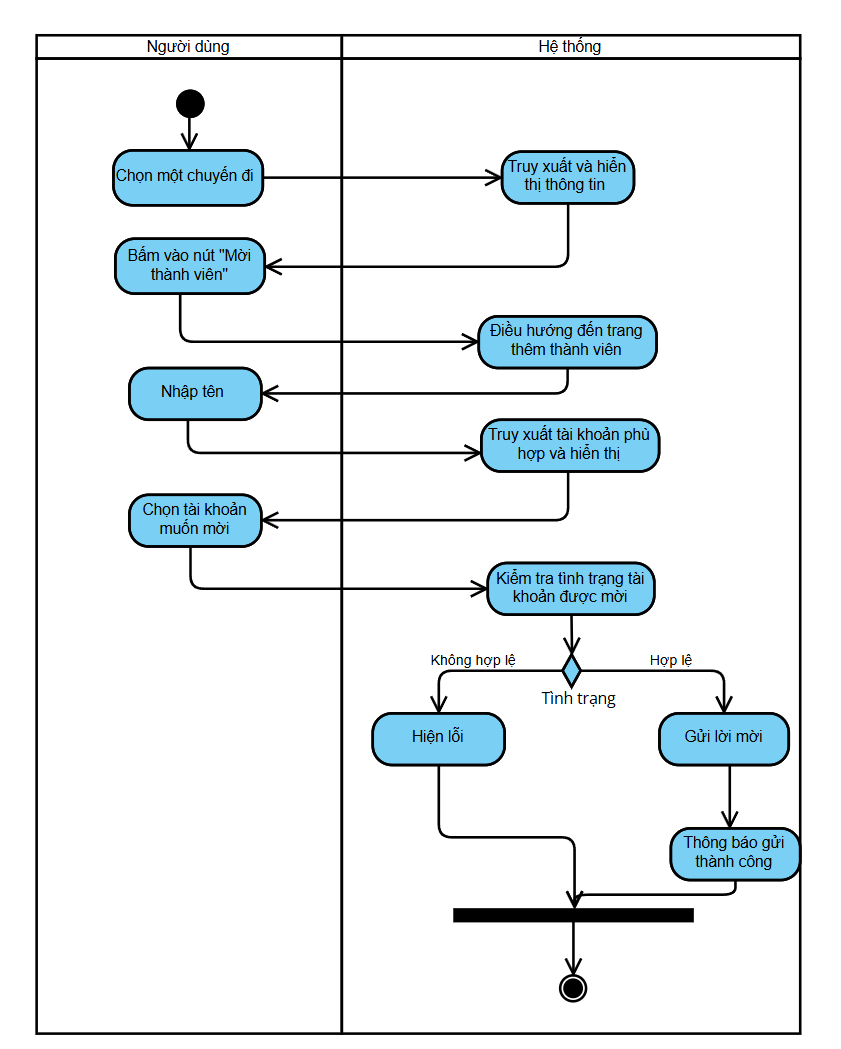
\includegraphics[width=0.5\linewidth]{figures/c3/3-3-14-ad.png} % Specified width
        &
        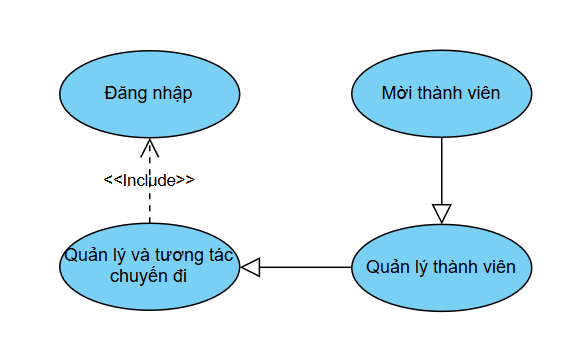
\includegraphics[width=0.45\linewidth]{figures/c3/3-3-14-rd.png} \\ % Specified width
        \hline
    \end{tabular}
\end{table}

\begin{figure}[H]
    \centering
    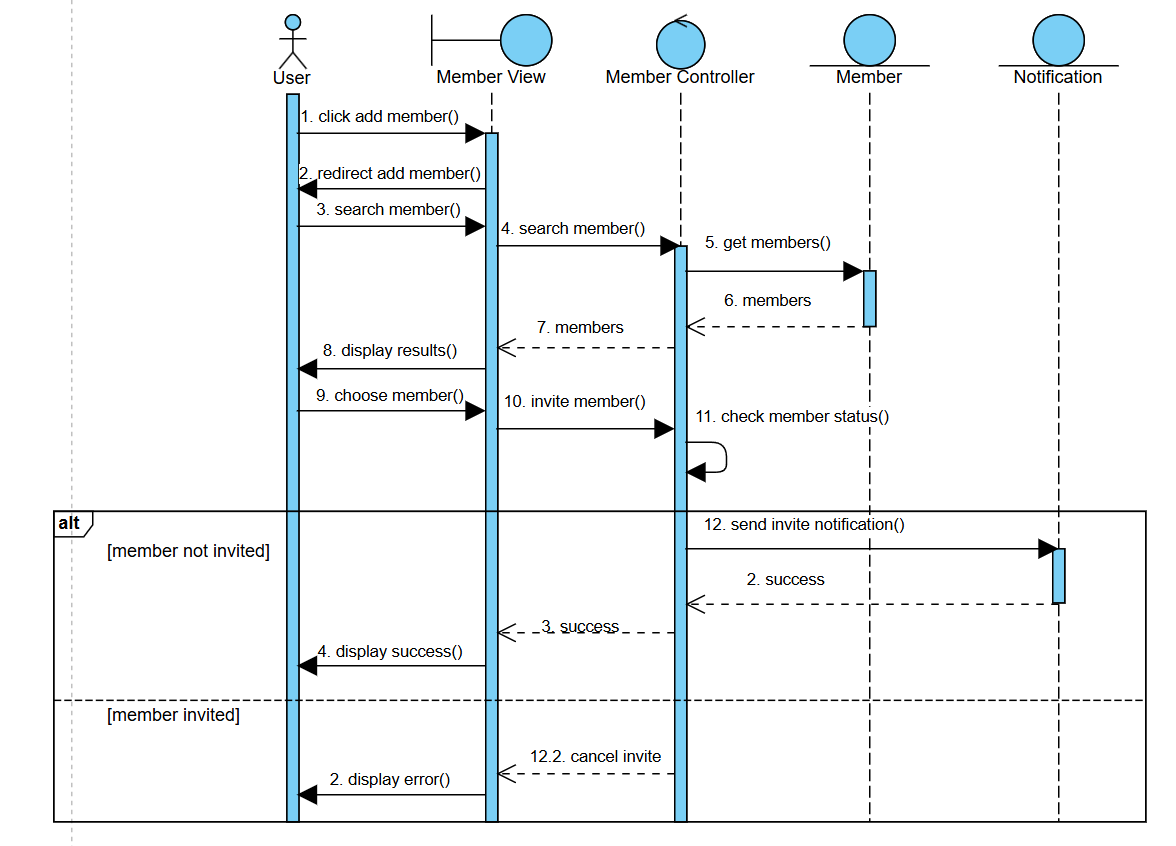
\includegraphics[width=0.85\textwidth]{figures/c3/3-3-14-sd.png} % Specified width
    \caption{Biểu đồ tuần tự ca sử dụng mời bạn bè tham gia chuyến đi.} % (no period)
    \label{fig:3-3-14-sequence-diagram}
\end{figure}
% \nopagebreak
% \subsection{Ca sử dụng công khai chuyến đi}
\vspace{0.5cm}


\noindent 
\begin{tabularx}{\linewidth}{| l | X |} 
\hline 
\textbf{Mô tả} & Người dùng công khai chuyến đi để mọi người tham gia. \\
\hline 
\textbf{Luồng cơ bản} & 1. Người dùng chọn một chuyến đi muốn công khai. \newline
                        2. Hệ thống lây dữ liệu chi tiết của chuyến đi và hiển thị. \newline
                        3. Người dùng bấm "Công khai". \newline
                        4. Hệ thống kiểm tra thông tin chuyến đi. \newline
                        5. Hệ thống chuyển đổi chuyến đi sang công khai và thông báo đến các tài khoản khác. \\
             
               
\hline 
\textbf{Luồng thay thế} & Chuyến đi không đủ thông tin hệ thống sẽ thông báo lỗi chưa đủ thông tin. \\
       
\hline 
\textbf{Tiền điều kiện} & - Người dùng đang đăng nhập và phiên đăng nhập chưa kết thúc.\newline
                        - Người dùng đã tạo ít nhất một chuyến đi. \newline
                        - Chuyến đi phải là chuyến di riêng tư.\\


\hline 
\textbf{Hậu điều kiện} & - Hệ thống cập nhật quyền riêng tư của chuyến đi sang công khai. \newline
- Hệ thống hiển thị chuyến đi dưới dạng bài viết trên trang chủ để mọi người tham gia. \newline
- Hệ thống gửi thông báo đến các tài khoản khác về chuyến đi công khai. \\
                        

\hline 
\textbf{Yêu cầu phi chức năng} & Hệ thống công khai chuyến đi dưới 2s \\
\hline 
\end{tabularx}

\noindent 
\begin{tabular}{| c | c |}
    \hline
    \textbf{Biểu đồ hoạt động} & \textbf{Quan hệ} \\ 
    \hline
    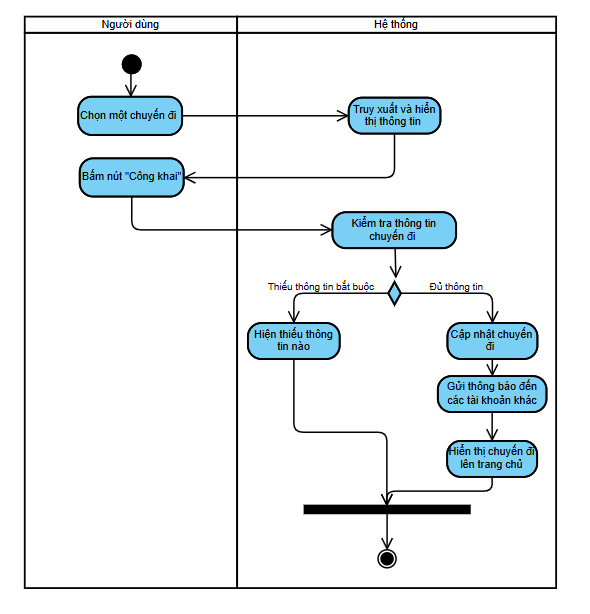
\includegraphics[width=0.5\linewidth]{figures/c3/3-3-15-ad.png} 
    & 
    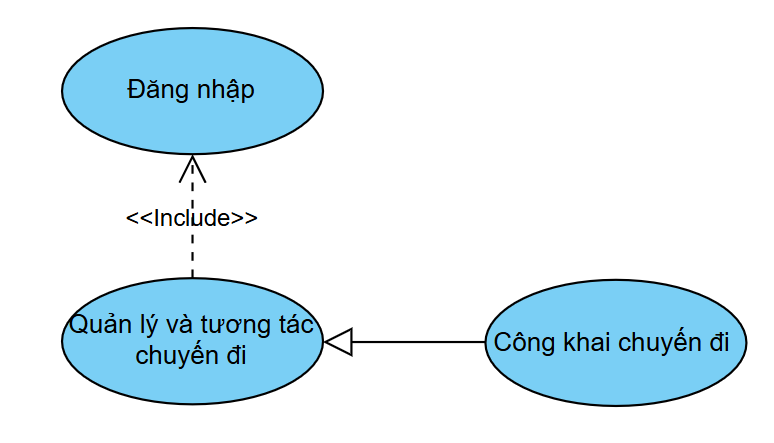
\includegraphics[width=0.45\linewidth]{figures/c3/3-3-15-rd.png} \\ 
    \hline
\end{tabular}

\vspace{0.8cm}

\begin{figure}[H]
    \centering  
    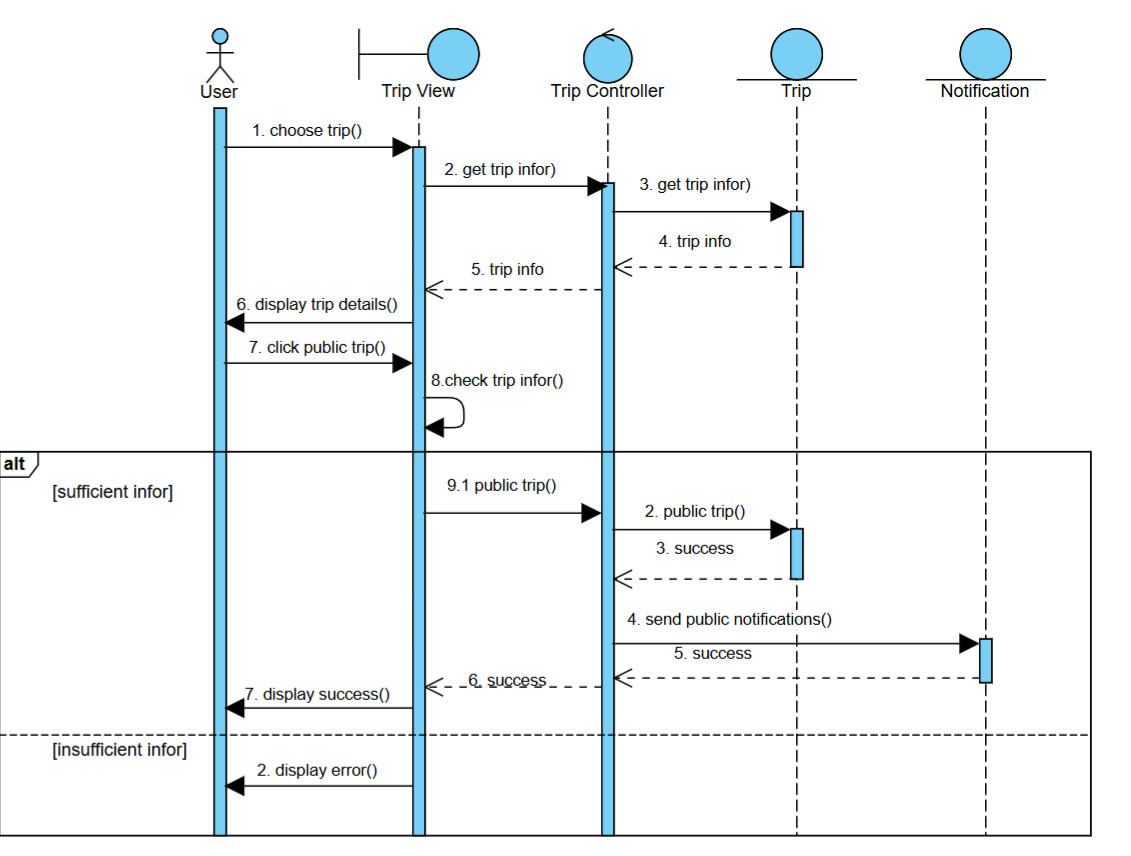
\includegraphics[width=1\textwidth]{figures/c3/3-3-15-sd.png}
    \caption{Biểu đồ tuần tự ca sử dụng công khai chuyến đi.}
    \label{fig:3-3-15-sequence-diagram}
\end{figure}
% \nopagebreak
\subsection{Ca sử dụng chia sẻ vị trí}
\noindent Ca sử dụng này mô tả cách người dùng chia sẻ vị trí thời gian thực của họ với các thành viên khác trong cùng một chuyến đi đang diễn ra. Tính năng này giúp các thành viên dễ dàng tìm thấy nhau hoặc theo dõi tiến trình di chuyển. Bảng~\ref{tab:uc_share_location_spec} trình bày chi tiết đặc tả ca sử dụng, bao gồm luồng sự kiện chính, luồng thay thế, các điều kiện và yêu cầu liên quan. Các biểu đồ hoạt động, quan hệ (Bảng~\ref{tab:uc_share_location_diagrams}) và tuần tự (Hình~\ref{fig:3-3-16-sequence-diagram}) minh họa rõ hơn về quy trình và tương tác hệ thống.
% \vspace{0.5cm} % Adjust spacing if needed

% Use longtable environment
% Need \usepackage{longtable} and \usepackage{calc} in preamble
\begin{longtable}{| p{4cm} | p{\dimexpr\linewidth-4cm-4\tabcolsep} |} % Adjust widths as needed
    \caption{Đặc tả ca sử dụng chia sẻ vị trí} % Caption inside longtable (no period)
    \label{tab:uc_share_location_spec} \\ % Label after caption

    \hline
    \textbf{Mô tả} & Người dùng trong cùng chuyến đi có thể chia sẻ vị trí khi chuyến đi đang diễn ra. \\
    \hline
    \endfirsthead % Header for the first page

    % No \endhead content needed

    % No \endfoot content needed

    \hline % Footer for the last page
    \endlastfoot

    % --- Table Content ---
    \textbf{Luồng cơ bản} & 1. Người dùng chọn một chuyến đi đang diễn ra. \newline
                           2. Hệ thống lấy dữ liệu chi tiết của chuyến đi và hiển thị. \newline
                           3. Người dùng bấm ``Chia sẻ vị trí". \newline
                           4. Hệ thống điều hướng người dùng ra trang hiển thị bản đồ. \newline
                           5. Hệ thống yêu cầu quyền truy cập vị trí liên tục. \newline
                           6. Người dùng cấp quyền. \newline
                           7. Hệ thống cập nhật liên tục trong thời gian thực vị trí của bản thân người dùng và các người dùng khác tham gia chia sẻ vị trí trong chuyến đi. \\
    \hline
    \textbf{Luồng thay thế} & Nếu người dùng không cấp quyền truy cập vị trí, hệ thống sẽ không thể chia sẻ vị trí của họ và chỉ hiển thị vị trí của các thành viên khác (nếu có). \\
    \hline
    \textbf{Tiền điều kiện} & - Người dùng đang đăng nhập và phiên đăng nhập chưa kết thúc.\newline
                           - Người dùng đã tạo hoặc tham gia ít nhất một chuyến đi. \newline
                           - Chuyến đi đang trong trạng thái ``Đang diễn ra". \\
    \hline
    \textbf{Hậu điều kiện} & - Hệ thống cập nhật vị trí của người dùng và các người dùng khác trong chuyến đi trên bản đồ thời gian thực. \newline
                           - Hệ thống tạo thông báo đẩy trong thiết bị để chạy nền tác vụ chia sẻ vị trí. \\
    \hline
    \textbf{Yêu cầu phi chức năng} & - Hệ thống cập nhật vị trí trên bản đồ với độ trễ dưới 5 giây. \newline
                                   - Tính năng chia sẻ vị trí cần tối ưu để không tiêu tốn quá nhiều pin thiết bị. \\
    % --- End Table Content ---

\end{longtable}
\vspace{0.8cm}

\begin{table}[H] % Wrap the diagrams table
    \centering
    \caption{Biểu đồ hoạt động và quan hệ ca sử dụng chia sẻ vị trí} % Add caption (no period)
    \label{tab:uc_share_location_diagrams} % Add label
    \begin{tabular}{| c | c |}
        \hline
        \textbf{Biểu đồ hoạt động} & \textbf{Quan hệ} \\
        \hline
        \includegraphics[width=0.5\linewidth]{figures/c3/3-3-16-ad.png} % Specified width
        &
        \includegraphics[width=0.45\linewidth]{figures/c3/3-3-16-rd.png} \\ % Specified width
        \hline
    \end{tabular}
\end{table}

\begin{figure}[H]
    \centering
    \includegraphics[width=1\textwidth]{figures/c3/3-3-16-sd.png} % Specified width
    \caption{Biểu đồ tuần tự ca sử dụng chia sẻ vị trí} % (no period)
    \label{fig:3-3-16-sequence-diagram}
\end{figure}
\nopagebreak
% \input{chapters/c3/usecases_details/3.3.17_uc}\nopagebreak\newpage\cleardoublepage
% \chapter{TRIỂN KHAI VÀ KIỂM THỬ ỨNG DỤNG}
\label{chap:experiment}

% \section{Triển khai hệ thống}
% Mục này đi sâu vào các khía cạnh kỹ thuật chính trong quá trình xây dựng và triển khai các thành phần của hệ thống VieVu. Các nội dung chính được trình bày trong mục này bao gồm phương pháp thu thập và chuẩn bị dữ liệu ban đầu, chi tiết triển khai kỹ thuật cho các module AI cốt lõi (hệ thống tổng hợp tin nhắn và hệ thống gợi ý), và tổng quan về kiến trúc triển khai cuối cùng của toàn bộ hệ thống.

% \input{chapters/c4/system_design/4.1.1/4.1.1_video_design.tex}

% \input{chapters/c4/system_design/4.1.2/4.1.2_design_system.tex}

\subsection{Thu thập dữ liệu}


Để ứng dụng VieVu có thể hoạt động và cung cấp các chức năng cốt lõi như tìm kiếm, hiển thị thông tin, và gợi ý, việc xây dựng một bộ dữ liệu nền tảng ban đầu là bước thiết yếu. Dữ liệu ban đầu này bao gồm thông tin chi tiết về các địa điểm du lịch (attractions), các điểm đến lớn hơn (locations - tỉnh, quận,v.v.) và các loại hình du lịch (travel types).

\subsubsection{Nguồn và phương pháp thu thập dữ liệu}
Hệ thống thu thập dữ liệu từ hai nguồn chính là nền tảng \textbf{vn.trip.com} (cho dữ liệu chính về địa điểm, điểm đến, loại hình, và các thông tin khác) và \textbf{Ticketbox} (cho thông tin về các sự kiện).

Việc thu thập dữ liệu từ \texttt{vn.trip.com} gặp phải thách thức khi các yêu cầu truy cập trực tiếp bị chặn. Để giải quyết vấn đề này phải xây dựng một \textbf{proxy server bằng Node.js và TypeScript}. Proxy server này đóng vai trò trung gian, xử lý các yêu cầu đến \texttt{vn.trip.com} và cho phép việc thu thập dữ liệu diễn ra.

Trong quá trình thu thập, nhận thấy dữ liệu về mô tả (\texttt{description}) và phân loại loại hình du lịch (\texttt{travel\_type}) cho một số điểm tham quan bị thiếu hoặc chưa đầy đủ. Vì lý do này hệ thống đã tích hợp sử dụng \textbf{API của Google Gemini} để tự động tạo ra các mô tả và thông tin loại hình còn thiếu dựa trên thông tin có sẵn khác của điểm tham quan.

\subsubsection{Kết quả thu thập dữ liệu}
Thông qua quá trình crawling từ \texttt{vn.trip.com}, một bộ dữ liệu ban đầu đáng kể đã được thu thập và lưu trữ vào cơ sở dữ liệu PostgreSQL của hệ thống (quản lý bởi Supabase), bao gồm:
\begin{itemize}
    \item \textbf{1006 } bản ghi điểm tham quan (\texttt{attractions}), chứa các thông tin như tên, mô tả, ảnh bìa (\texttt{cover}), danh sách URL ảnh (\texttt{images}), điểm đánh giá (\texttt{hot\_score}, \texttt{avg\_rating}, \texttt{rating\_count}), giá tham khảo (\texttt{price}), tọa độ địa lý (\texttt{latitude}, \texttt{longitude}), địa chỉ (\texttt{address}), quy tắc giờ mở cửa (\texttt{open\_time\_rule}), và khóa ngoại liên kết đến địa điểm lớn (\texttt{location\_id}).
    \item \textbf{538} bản ghi điểm đến (\texttt{locations}), chủ yếu là các tỉnh/thành phố, quận của Việt Nam, chứa tên, ảnh, tọa độ và liên kết cha-con (nếu có).
    \item \textbf{100} bản ghi loại hình du lịch (\texttt{travel\_types}), bao gồm 12 loại hình cha và 88 loại hình con, lưu trữ dưới dạng ID (\texttt{id} dạng text) và tên (\texttt{name}).
    \item Bảng liên kết \textbf{\texttt{attraction\_types}} được tạo ra để quản lý mối quan hệ nhiều-nhiều giữa điểm tham quan và loại hình du lịch.
\end{itemize}
Các bảng này (\texttt{attractions}, \texttt{locations}, \texttt{travel\_types}, \texttt{attraction\_types}) được thiết kế với các khóa chính, khóa ngoại và chỉ mục (indexes) phù hợp như đã mô tả trong phần thiết kế CSDL (Mục \ref{sec:3-4-database}).

\subsubsection{Mục đích sử dụng dữ liệu}
Bộ dữ liệu được thu thập và làm giàu này đóng vai trò kép: (1) Cung cấp nội dung nền tảng phong phú cho các chức năng hiển thị, tra cứu, lọc thông tin địa điểm trên ứng dụng VieVu dành cho người dùng cuối. (2) Làm dữ liệu đầu vào quan trọng cho việc huấn luyện các mô hình gợi ý (recommendation models) sẽ được trình bày ở các mục sau.
Quá trình thu thập và chuẩn bị dữ liệu ban đầu này, dù gặp một số thách thức kỹ thuật, đã tạo ra nền tảng dữ liệu cần thiết cho sự hoạt động và phát triển của các tính năng cốt lõi trong hệ thống VieVu.



\subsection{Tổng hợp tin nhắn tạo lịch trình}
\label{subsec:summary_implementation_revised} % Label mới cho subsection

Một trong những tính năng ứng dụng AI nổi bật của VieVu là khả năng phân tích nội dung hội thoại trong nhóm chat và tự động đề xuất bản nháp lịch trình chi tiết cho chuyến đi. Để hiện thực hóa tính năng này một cách hiệu quả, tránh việc phải xử lý lại toàn bộ lịch sử trò chuyện mỗi khi người dùng yêu cầu, một kiến trúc xử lý gồm hai giai đoạn chính đã được thiết kế và triển khai trên nền tảng server FastAPI.

\subsubsection{Giai đoạn 1: Tiền xử lý Tin nhắn Bất đồng bộ}
\label{subsubsec:summary_phase1_revised}

Giai đoạn đầu tiên của pipeline tập trung vào việc xử lý các tin nhắn mới ngay khi chúng được gửi đến hệ thống, nhằm mục đích phân loại và trích xuất thông tin liên quan một cách tự động và bất đồng bộ.

Đầu tiên, để phát hiện tin nhắn mới một cách hiệu quả, hệ thống sử dụng cơ chế \textbf{LISTEN/NOTIFY} tích hợp sẵn của PostgreSQL. Một trigger cơ sở dữ liệu được cấu hình trên bảng \texttt{messages} để mỗi khi có một bản ghi mới được chèn, nó sẽ gửi một thông báo đến kênh \texttt{messages\_insert}, kèm theo dữ liệu (payload) của tin nhắn mới dưới dạng JSON, như minh họa trong Đoạn mã~\ref{lst:json-payload}. % (Xem chi tiết trigger tại Phụ lục \ref{apdx:db_trigger}) % <<< Placeholder

\lstset{language=json}
\begin{lstlisting}[
    caption=Payload JSON của tin nhắn mới (dạng dictionary Python),
    label=lst:json-payload,
    captionpos=t,
    belowcaptionskip=10pt,
    basicstyle=\small\ttfamily,
    breaklines=true,
    showstringspaces=false,
    inputencoding=utf8]
{
    "id": 335,
    "created_at": "2025-04-23T03:54:26.25777+00:00",
    "content": "Thu den Vinh Ha Long xem the nao cung duoc",
    "chat_id": 1,
    "meta_data": None,
    "is_travel_related": None,
    "chat_member_id": 10
}
\end{lstlisting}

\noindent Phía server FastAPI, một tác vụ nền \texttt{listen\_to\_messages} sử dụng thư viện \texttt{asyncio} của Python được khởi chạy và duy trì hoạt động liên tục nhờ cơ chế quản lý vòng đời \texttt{lifespan} của FastAPI. Tác vụ này thực hiện lệnh \texttt{LISTEN messages\_insert;} để lắng nghe các thông báo được gửi từ PostgreSQL trên kênh đã định. % (Xem mã nguồn hàm lắng nghe tại Đoạn mã \ref{lst:listener_code}) % <<< Placeholder

Tiếp theo là bước xử lý dữ liệu tin nhắn nhận được. Khi tác vụ nền nhận được dữ liệu payload của tin nhắn mới, nó thực hiện tuần tự các bước sau. Trước hết, nội dung tin nhắn được đưa vào hàm \texttt{classify\_sentence()} để thực hiện phân loại Zero-Shot  ZSC, sử dụng mô hình \texttt{joeddav/xlm-roberta-large-xnli} với hai nhãn \texttt{"travel schedule information"} và \texttt{"not travel schedule information"}. Kết quả phân loại, ví dụ như trong Đoạn mã~\ref{lst:zsc_output}, được dùng để xác định giá trị boolean \texttt{is\_travel\_related} dựa trên điểm tin cậy của nhãn \texttt{"travel schedule information"} $\geq 0.4$.

\lstset{language=json}
\begin{lstlisting}[
    caption=Output phân loại của mô hình ZSC (dạng dictionary Python),
    label=lst:zsc_output,
    captionpos=t,
    belowcaptionskip=10pt,
    basicstyle=\small\ttfamily,
    breaklines=true,
    showstringspaces=false,
    inputencoding=utf8]
{
    "sequence": "Thu den Vinh Ha Long xem the nao cung duoc",
    "labels": ["travel schedule information", "not travel schedule information"],
    "scores": [0.5240467190742493, 0.4759533107280731]
}
\end{lstlisting}

\noindent Nếu tin nhắn được xác định là liên quan (\texttt{is\_travel\_related = true}), bước nhận dạng tên địa điểm (NER) được thực hiện. Nội dung tin nhắn được xử lý bởi hàm \texttt{get\_place\_name()} (sử dụng thư viện \texttt{underthesea}). Các thực thể địa điểm mới tìm thấy, như minh họa trong kết quả tại Đoạn mã~\ref{lst:ner_output}, sẽ được định dạng và bổ sung vào trường \texttt{meta\_data} (JSONB) của tin nhắn, đồng thời tránh lưu trữ trùng lặp thông tin đã có.

\lstset{language=Python} % Giả định output này là tuple Python
\begin{lstlisting}[
    caption=Output nhận dạng thực thể của thư viện Underthesea,
    label=lst:ner_output,
    captionpos=t,
    belowcaptionskip=10pt,
    basicstyle=\small\ttfamily,
    breaklines=true,
    showstringspaces=false,
    inputencoding=utf8]
[
    ("Thu", "V", "B-VP", "O"),
    ("den", "E", "B-PP", "O"),
    ("Vinh", "N", "B-NP", "B-LOC"),
    ("Ha Long", "Np", "I-NP", "I-LOC"),
    ("xem", "V", "B-VP", "O"),
    ("the nao", "P", "B-NP", "O"),
    ("cung", "R", "O", "O"),
    ("duoc", "V", "B-VP", "O")
]
\end{lstlisting}

\noindent Sau đó, hệ thống áp dụng logic fallback để xử lý phản hồi khẳng định/phủ định. Cụ thể, nếu tin nhắn trước đó liên quan nhưng tin nhắn hiện tại không, hàm \texttt{classify\_affirmative()} (cũng dùng mô hình ZSC với các nhãn \texttt{"affirmation or negation"} và \texttt{"not affirmation and negation"}) sẽ kiểm tra xem đây có phải lời khẳng định/phủ định không. Nếu đúng, \texttt{is\_travel\_related} sẽ được đặt lại thành \texttt{true}. Cuối cùng, việc cập nhật cơ sở dữ liệu được thực hiện, lưu giá trị \texttt{is\_travel\_related} và trường \texttt{meta\_data} đã xử lý vào bản ghi tin nhắn tương ứng trong bảng \texttt{messages}. % (Xem chi tiết logic xử lý tại Đoạn mã \ref{lst:message_processing_logic}) % <<< Placeholder

Cuối cùng, trong Giai đoạn 1, hệ thống chuẩn bị thêm khâu xử lý dữ liệu tồn đọng. Để đảm bảo không bỏ sót tin nhắn gửi trong lúc server không hoạt động, hàm \texttt{update\_travel\_related\_status()} được thực thi khi server khởi động, thực hiện toàn bộ luồng xử lý ZSC, NER, Affirmation Check cho các tin nhắn có \texttt{is\_travel\_related} là NULL.

Kết thúc Giai đoạn 1, các tin nhắn trong cơ sở dữ liệu đã được phân loại và xử lý thông tin một cách tự động, tạo tiền đề dữ liệu cần thiết và tối ưu cho Giai đoạn 2.

\subsubsection{Giai đoạn 2: Tổng hợp và Tạo Lịch trình theo Yêu cầu}
\label{subsubsec:summary_phase2_revised}

Sau khi tin nhắn được tiền xử lý, Giai đoạn 2 được kích hoạt bởi người dùng để tạo bản nháp lịch trình cuối cùng, phối hợp giữa client (Flutter) và server (FastAPI).

Đầu tiên là bước chuẩn bị dữ liệu phía Client. Khi người dùng yêu cầu, ứng dụng Flutter truy vấn các tin nhắn liên quan mới nhất từ Supabase (đã được đánh dấu \texttt{is\_travel\_related=true}, mới hơn tin nhắn cuối được tổng hợp) kèm theo thông tin \texttt{message\_reactions}. Client tự xử lý logic vote từ reaction like/dislike để tạo marker `|Yes|` hoặc `|No|` nối vào cuối nội dung các tin nhắn tương ứng. Đồng thời, client thu thập metadata địa điểm, ngày đi và lịch trình cũ (nếu có).

Tiếp theo, client thực hiện gọi API tổng hợp phía Server. Client Flutter tạo JSON body chứa danh sách \texttt{conversation} (đã xử lý vote), \texttt{metadata}, \texttt{start\_date}, \texttt{end\_date}, và \texttt{previous\_summary} (nếu có), rồi gửi yêu cầu POST đến endpoint \texttt{/summarize} của server FastAPI cùng token xác thực. Cấu trúc JSON request hoàn chỉnh được minh họa trong Hình~\ref{fig:input}. % (Tham khảo mã gọi API tại Đoạn mã \ref{lst:client_api_call}) % <<< Placeholder
    \begin{figure}[H]
        \centering
        \includegraphics[width=0.8\textwidth]{figures/c4/input.png}
        \caption{JSON request hoàn chỉnh từ client gửi đến server.}
        \label{fig:input}
    \end{figure}

Sau đó, phía server thực hiện xây dựng Prompt. Server FastAPI nhận yêu cầu, tổng hợp dữ liệu và xây dựng một prompt chi tiết cho Google Gemini API (model flash 2.5), như minh họa trong Hình~\ref{fig:prompt}. Prompt này chứa đầy đủ ngữ cảnh và các chỉ dẫn cụ thể về cách tạo lịch trình dạng JSON theo yêu cầu (lọc sự kiện, xử lý Yes/No, liên kết metadata, gộp lịch trình cũ, tuân thủ định dạng output, v.v.). % (Tham khảo cấu trúc prompt chi tiết tại Phụ lục \ref{apdx:gemini_prompt}) % <<< Placeholder
    \begin{figure}[H]
        \centering
        \includegraphics[width=0.9\textwidth]{figures/c4/prompt2.png}
        \caption{Prompt hướng dẫn Gemini tổng hợp lịch trình.}
        \label{fig:prompt}
    \end{figure}

Cuối cùng là bước xử lý kết quả, lưu trữ và phản hồi. Server FastAPI gửi prompt đến Gemini API, nhận phản hồi JSON chứa lịch trình, phân tích cú pháp kết quả đó. Sau đó, server thực hiện thao tác \texttt{upsert} vào bảng \texttt{chat\_summaries} để lưu/cập nhật lịch trình (\texttt{summary}), bản đọc (\texttt{readings}), và \texttt{last\_message\_id}. Kết quả lịch trình cuối cùng (ví dụ như trong Hình~\ref{fig:output}) được gửi về client Flutter để hiển thị.
    \begin{figure}[H]
        \centering
        \includegraphics[width=0.8\textwidth]{figures/c4/output.png}
        \caption{Output JSON chứa lịch trình trả về từ server.}
        \label{fig:output}
    \end{figure}

Kiến trúc xử lý hai giai đoạn này, kết hợp tiền xử lý bất đồng bộ và tổng hợp thông minh theo yêu cầu bằng LLM, cho phép VieVu cung cấp tính năng hỗ trợ tạo lịch trình mạnh mẽ và hiệu quả.



\subsection{Triển khai Hệ thống Gợi ý}
\label{subsec:recsys_implementation_paragraph} % Label mới

Hệ thống VieVu triển khai hai cơ chế gợi ý chính để đề xuất địa điểm cho người dùng. Mục này trình bày chi tiết việc triển khai kỹ thuật cho cả hai cơ chế: gợi ý địa điểm liên quan dựa trên nội dung (Content-Based) và gợi ý địa điểm chính dựa trên Neural Network (Hybrid).

\subsubsection{Gợi ý Địa điểm Liên quan (Content-Based)}
\label{subsubsec:cb_recsys_impl_paragraph_final} % Label mới

Hệ thống gợi ý địa điểm liên quan hoạt động bằng cách kết hợp điểm đánh giá chất lượng/phổ biến nội tại của địa điểm với độ tương đồng về mặt nội dung văn bản. Đầu tiên, một điểm số nội tại ($Score_{Item}$) cho mỗi điểm tham quan được tính toán. Điểm này dựa trên điểm đánh giá trung bình có trọng số ($Score_{WeightedAvg}$) được làm mượt bằng công thức:
$$Score_{WeightedAvg} = \frac{R \times v + C \times m}{v + m}$$
Trong đó $R$ là điểm trung bình gốc, $v$ là số lượt đánh giá, $C$ là điểm trung bình toàn cục, và $m$ là ngưỡng tối thiểu. Sau đó, giá trị $Score_{WeightedAvg}$ và \texttt{hot\_score} được chuẩn hóa về thang [0, 1] ($ScaledWeightedAvg$, $ScaledHotScore$) và kết hợp thành $Score_{Item}$ cuối cùng với trọng số $w_{hs}=0.6, w_{wa}=0.4$:
$$Score_{Item} = w_{hs} \times ScaledHotScore + w_{wa} \times ScaledWeightedAvg$$
% (Tham khảo mã nguồn tại Đoạn mã \ref{lst:score_calculation}) % <<< Placeholder

Tiếp theo, nội dung văn bản của các địa điểm được tiền xử lý, tổng hợp thành trường \texttt{bag\_of\_words} và vector hóa bằng \texttt{TfidfVectorizer} từ Scikit-learn~\cite{sklearn_lib} (có loại bỏ từ dừng tiếng Việt) để tạo ma trận TF-IDF. Độ tương đồng nội dung giữa hai địa điểm (vector $\vec{a}$ và $\vec{b}$) được đo bằng Cosine Similarity:
$$\text{Cosine Similarity}(\vec{a}, \vec{b}) = \frac{\vec{a} \cdot \vec{b}}{\|\vec{a}\| \|\vec{b}\|}$$
Kết quả là ma trận độ tương đồng \texttt{cos\_sim} giữa các cặp địa điểm. % (Tham khảo tại Đoạn mã \ref{lst:tfidf_cosine_code}) % <<< Placeholder

Cuối cùng, hàm gợi ý \texttt{get\_related\_attractions} được triển khai. Hàm này nhận ID địa điểm đang xem, lấy $Score_{Item}$ và độ tương đồng nội dung ($Similarity$) từ \texttt{cos\_sim}, rồi tính điểm gợi ý cuối cùng ($Score_{Final}$) bằng cách kết hợp chúng với trọng số $w_{sim}$ (ví dụ: 0.7):
$$Score_{Final} = w_{sim} \times Similarity + (1 - w_{sim}) \times Score_{Item}$$
Top N địa điểm có $Score_{Final}$ cao nhất (trừ địa điểm gốc) được trả về thông qua API endpoint của FastAPI. % (Tham khảo tại Đoạn mã \ref{lst:related_attractions_func}) % <<< Placeholder

\subsubsection{Gợi ý Địa điểm Chính (Neural Network - Hybrid)}
\label{subsubsec:nn_recsys_impl_paragraph_final} % Label mới

Hệ thống gợi ý chính của VieVu, nhằm đề xuất địa điểm cá nhân hóa, được xây dựng dựa trên mô hình Neural Network (NN) theo cách tiếp cận Hybrid, sử dụng thư viện TensorFlow và Keras~\cite{tensorflow_lib, keras_lib}. Mô hình này dự đoán mức độ phù hợp (rating dự đoán) dựa trên sự kết hợp của ba nguồn thông tin: đặc trưng người dùng (User Features từ khảo sát/hành vi), đặc trưng địa điểm (Item Features gồm thuộc tính số và OHE loại hình), và dữ liệu đánh giá giả lập.

Quá trình chuẩn bị dữ liệu bao gồm tải dữ liệu đặc trưng cho khoảng 3500 người dùng và 1006 địa điểm. Do hạn chế dữ liệu rating thực tế, bộ dữ liệu huấn luyện (\texttt{user\_ratings\_data.csv}) được tạo giả lập bằng cách phân phối ngẫu nhiên điểm rating cho cặp (user, item) dựa trên thống kê gốc (\texttt{avg\_rating}, \texttt{rating\_count}) của địa điểm. Dữ liệu đặc trưng và rating giả lập sau đó được kết hợp và chia thành tập huấn luyện (90%) và kiểm thử (10%).

Mô hình NN được thiết kế theo kiến trúc two-tower song song. Nhánh người dùng và nhánh địa điểm nhận đầu vào là các vector đặc trưng tương ứng, mỗi nhánh đi qua hai lớp Dense (128 và 64 nơ-ron, ReLU). Output từ hai nhánh được ghép nối (Concatenate), đi qua một lớp Dense (64 nơ-ron, ReLU) và lớp Dense output cuối cùng (1 nơ-ron, 'linear') để dự đoán rating. Chi tiết thiết lập các lớp mạng được thể hiện trong Đoạn mã~\ref{lst:nn_model}. % (Sơ đồ kiến trúc có thể xem tại Hình~\ref{fig:nn_arch}) % <<< Placeholder

\lstset{language=python}
\begin{lstlisting}[
    caption=Thiết lập các lớp chính của mô hình Neural Network,
    label=lst:nn_model,
    captionpos=t,
    belowcaptionskip=10pt,
    basicstyle=\small\ttfamily,
    breaklines=true,
    showstringspaces=false,
    inputencoding=utf8]
    # User branch
    user_layer = Dense(128, activation="relu")(input_user)
    user_layer = Dense(64, activation="relu")(user_layer)
    # Attraction branch
    attraction_layer = Dense(128, activation="relu")(input_attraction)
    attraction_layer = Dense(64, activation="relu")(attraction_layer)
    # Merge and predict
    merged = Concatenate()([user_layer, attraction_layer])
    merged = Dense(64, activation="relu")(merged)
    output = Dense(1, activation="linear")(merged)
    
\end{lstlisting}

Mô hình được huấn luyện để tối thiểu hóa Mean Squared Error (MSE) giữa rating dự đoán và rating giả lập, sử dụng optimizer Adam (learning rate 0.001) và theo dõi Mean Absolute Error (MAE). Quá trình huấn luyện diễn ra trong 30 epochs với batch size 32. Kết quả huấn luyện được trực quan hóa trong Hình~\ref{fig:mae} cho thấy mô hình học được từ dữ liệu (Loss và MAE đều giảm) và đạt MAE khoảng 0.64 trên tập kiểm chứng, mặc dù có dấu hiệu overfitting. Mô hình với trọng số tốt nhất được lưu lại. % <<< NHỚ THAY LABEL FIG ĐÚNG !!!
    \begin{figure}[H]
        \centering
        \includegraphics[width=\textwidth]{figures/c4/128.png} % Đường dẫn tới file ảnh của bạn
        \caption{Hiệu suất mô hình qua độ đo MAE và Loss trong quá trình huấn luyện.} % Cập nhật caption
        \label{fig:mae} % Giữ nguyên label nếu bạn đã dùng
    \end{figure}

Như vậy, việc triển khai hệ thống gợi ý địa điểm chính của VieVu đã hoàn thành thông qua việc xây dựng và huấn luyện mô hình Neural Network Hybrid. Bằng cách kết hợp thông tin đặc trưng và tín hiệu học hỏi từ dữ liệu rating giả lập, mô hình được tối ưu hóa để dự đoán mức độ phù hợp. Hệ thống gợi ý cuối cùng được tích hợp vào API server, sẵn sàng cung cấp các đề xuất địa điểm cá nhân hóa cho người dùng.


\subsection{Kiến trúc Hệ thống}
\label{subsec:system_architecture_impl}

Kiến trúc tổng thể của hệ thống VieVu khi triển khai là sự kết hợp giữa ứng dụng client (Flutter), nền tảng Backend as a Service (Supabase) và một backend tùy chỉnh (Python/FastAPI) cho các tác vụ chuyên biệt. Sơ đồ Hình~\ref{fig:system_architecture} minh họa các thành phần chính và luồng tương tác dữ liệu giữa chúng.

\begin{figure}[H]
    \centering
    \includegraphics[width=1\textwidth]{figures/c4/architecture.png}
    \caption{Kiến trúc tổng thể của hệ thống VieVu.}
    \label{fig:system_architecture}
\end{figure}
\begin{enumerate}
    \item[-]\textbf{Người dùng (User):} Tác nhân chính tương tác với hệ thống thông qua ứng dụng client.
    \item[-]\textbf{Flutter Client:} Ứng dụng di động được xây dựng bằng Flutter, là giao diện chính để người dùng thực hiện các hành động như xem thông tin, lập kế hoạch, nhắn tin, yêu cầu gợi ý, v.v.
    \item[-]\textbf{Flutter Background Service:} Một dịch vụ chạy nền trên thiết bị người dùng (triển khai bằng Flutter), có thể dùng để xử lý thông báo hoặc đồng bộ dữ liệu nền tảng.
    \item[-]\textbf{Supabase Service:} Nền tảng BaaS cung cấp các dịch vụ backend cốt lõi, bao gồm:
        \begin{itemize}
            \item[-]\texttt{Supabase Authentication server:} Xử lý xác thực người dùng.
            \item[-]\texttt{Supabase database server:} Cung cấp API để tương tác trực tiếp với CSDL PostgreSQL.
            \item[-]\texttt{PostgreSQL Database:} Nơi lưu trữ dữ liệu chính của ứng dụng.
            \item[-]\texttt{Supabase Realtime server:} Quản lý các kết nối thời gian thực và phát các thay đổi dữ liệu.
        \end{itemize}
    \item[-]\textbf{Python Backend:} Backend tùy chỉnh được xây dựng để xử lý các tác vụ phức tạp, bao gồm:
        \begin{itemize}
            \item[-]\texttt{FastAPI Server:} Cung cấp các API endpoint cho các chức năng AI và tìm kiếm/tổng hợp.
            \item[-]\texttt{AI Models:} Các mô hình AI/ML đã huấn luyện (NN gợi ý, NER, ZSC,v.v.) được tải và sử dụng bởi FastAPI server.
            \item[-]\texttt{Background tasks (FastAPI Lifespan):} Tác vụ nền chạy bất đồng bộ bao gồm phân loại, nhận dạng tên, để tiền xử lý tin nhắn.
        \end{itemize}
    \item[-]\textbf{External API:} Các API của bên thứ ba (ví dụ: Trip.com, Ticketbox) mà Python Backend tương tác để lấy dữ liệu.
\end{enumerate}




\noindent Kiến trúc kết hợp này cho phép VieVu tận dụng các dịch vụ mạnh mẽ, sẵn có và khả năng mở rộng của Supabase cho các tác vụ phổ thông, đồng thời sử dụng một backend Python/FastAPI tùy chỉnh, linh hoạt để triển khai các thuật toán AI/ML phức tạp và tích hợp với các nguồn dữ liệu bên ngoài, tạo nên một hệ thống hoàn chỉnh và hiệu quả.



% \section{Các chức năng chính}
\label{sec:system_function}

\noindent Phần này trình bày các chức năng chính được triển khai trong ứng dụng VieVu, minh họa bằng các hình ảnh giao diện thực tế. Các chức năng này bao gồm từ việc xác thực người dùng, khám phá thông tin du lịch, quản lý chuyến đi, đến các tính năng tương tác xã hội và ứng dụng AI như nhắn tin, tổng hợp lịch trình và gợi ý.

\subsection{Xác thực và Hồ sơ người dùng}
\noindent Hệ thống yêu cầu người dùng xác thực tài khoản thông qua việc đăng ký hoặc đăng nhập. Sau khi đăng ký thành công, người dùng được yêu cầu hoàn thành một khảo sát ngắn về sở thích du lịch (Hình~\ref{fig:func_pref}) để cá nhân hóa trải nghiệm. Mỗi người dùng có một trang hồ sơ cá nhân (Hình~\ref{fig:func_profile}) nơi họ có thể xem và cập nhật thông tin cơ bản của mình.

\begin{figure}[H]
    \centering
    \begin{subfigure}{0.326\textwidth}
        \includegraphics[width=1\linewidth]{figures/c4/system_func/sign_up.png}
        \caption{Form đăng ký}
        \label{fig:func_sign_up}
    \end{subfigure}
    \hfill
    \begin{subfigure}{0.326\textwidth}
        \includegraphics[width=1\linewidth]{figures/c4/system_func/pref.png}
        \caption{Khảo sát sở thích}
        \label{fig:func_pref}
    \end{subfigure}
    \hfill
    \begin{subfigure}{0.326\textwidth}
        \includegraphics[width=1\linewidth]{figures/c4/system_func/profile.png}
        \caption{Hồ sơ cá nhân}
        \label{fig:func_profile}
    \end{subfigure}
    \caption{Giao diện xác thực và hồ sơ người dùng.}
    \label{fig:auth-screen}
\end{figure}

\subsection{Trang chủ và Giới thiệu}
\noindent Sau khi xác thực, người dùng được dẫn đến màn hình giới thiệu ngắn gọn (Hình~\ref{fig:func_intro}) trước khi vào trang chính của ứng dụng. Trang chủ (Hình~\ref{fig:func_home}) là nơi hiển thị danh sách các chuyến đi công khai mà người dùng có thể tham gia. Chức năng tìm kiếm (Hình~\ref{fig:func_search_home}) cho phép lọc các chuyến đi theo từ khóa. Các giao diện này được minh họa trong Hình~\ref{fig:home-screen}.

\begin{figure}[H]
    \centering
    \begin{subfigure}{0.326\textwidth}
        \includegraphics[width=1\linewidth]{figures/c4/system_func/intro.png}
        \caption{Màn hình giới thiệu}
        \label{fig:func_intro}
    \end{subfigure}
    \hfill
    \begin{subfigure}{0.326\textwidth}
        \includegraphics[width=1\linewidth]{figures/c4/system_func/home.png}
        \caption{Trang chủ}
        \label{fig:func_home}
    \end{subfigure}
    \hfill
    \begin{subfigure}{0.326\textwidth}
        \includegraphics[width=1\linewidth]{figures/c4/system_func/search_home.png}
        \caption{Tìm kiếm chuyến đi}
        \label{fig:func_search_home}
    \end{subfigure}
    \caption{Giao diện giới thiệu và trang chủ.}
    \label{fig:home-screen}
\end{figure}

\subsection{Khám phá Thông tin Du lịch}
\noindent Người dùng có thể xem danh sách các địa điểm, sự kiện (Hình~\ref{fig:func_explore}), xem thông tin chi tiết và đánh giá của một địa điểm cụ thể (Hình~\ref{fig:func_att_detail}), hoặc trực quan hóa vị trí các địa điểm trên bản đồ (Hình~\ref{fig:func_map_loc}). Hệ thống cũng hỗ trợ tìm kiếm các dịch vụ lân cận vị trí hiện tại (Hình~\ref{fig:func_nearby}), tìm kiếm theo từ khóa (Hình~\ref{fig:func_search_loc}), và lọc kết quả theo tiêu chí như loại hình, giá, đánh giá (ví dụ lọc nhà hàng Hình~\ref{fig:func_filter_res}).

\begin{figure}[H]
    \centering
    % --- First Row ---
    \begin{subfigure}{0.326\textwidth}
        \includegraphics[height=10cm,width=1\linewidth]{figures/c4/system_func/explore.png}
        \caption{Trang Khám phá}
        \label{fig:func_explore}
    \end{subfigure}
    \hfill
    \begin{subfigure}{0.326\textwidth}
        \includegraphics[height=10cm,width=1\linewidth]{figures/c4/system_func/att.png}
        \caption{Chi tiết địa điểm}
        \label{fig:func_att_detail}
    \end{subfigure}
    \hfill
    \begin{subfigure}{0.326\textwidth}
        \includegraphics[height=10cm,width=1\linewidth]{figures/c4/system_func/map_loc.png}
        \caption{Xem trên bản đồ}
        \label{fig:func_map_loc}
    \end{subfigure}

    \vspace{\baselineskip} % Vertical space between rows

    % --- Second Row ---
    \begin{subfigure}{0.326\textwidth}
        \includegraphics[height=10cm,width=1\linewidth]{figures/c4/system_func/nearby.png}
        \caption{Địa điểm lân cận}
        \label{fig:func_nearby}
    \end{subfigure}
    \hfill
    \begin{subfigure}{0.326\textwidth}
        \includegraphics[height=10cm,width=1\linewidth]{figures/c4/system_func/res.png}
        \caption{Lọc địa điểm}
        \label{fig:func_filter_res}
    \end{subfigure}
    \hfill
    \begin{subfigure}{0.326\textwidth}
        \includegraphics[height=10cm,width=1\linewidth]{figures/c4/system_func/search.png}
        \caption{Tìm kiếm địa điểm}
        \label{fig:func_search_loc}
    \end{subfigure}

    \caption{Các giao diện chính của chức năng Khám phá.}
    \label{fig:explore-screens}
\end{figure}

\subsection{Quản lý Chuyến đi và Lịch trình}
\noindent Người dùng có thể tạo, tham gia và quản lý các chuyến đi. Trong mỗi chuyến đi, người dùng có thể xem và chỉnh sửa thông tin chung (Hình~\ref{fig:func_trip_info}), quản lý danh sách các địa điểm/dịch vụ đã lưu để cân nhắc (Hình~\ref{fig:func_saved_service}), và quản lý thành viên tham gia (Hình~\ref{fig:func_manage_member}), như minh họa trong Hình~\ref{fig:trip-management-1}.

\begin{figure}[H]
    \centering
    \begin{subfigure}{0.326\textwidth}
        \includegraphics[width=1\linewidth]{figures/c4/system_func/tripinfo.png}
        \caption{Thông tin chuyến đi}
        \label{fig:func_trip_info}
    \end{subfigure}
    \hfill
    \begin{subfigure}{0.326\textwidth}
        \includegraphics[width=1\linewidth]{figures/c4/system_func/save_service.png}
        \caption{Địa điểm đã lưu}
        \label{fig:func_saved_service}
    \end{subfigure}
    \hfill
    \begin{subfigure}{0.326\textwidth}
        \includegraphics[width=1\linewidth]{figures/c4/system_func/manage_member.png}
        \caption{Quản lý thành viên}
        \label{fig:func_manage_member}
    \end{subfigure}
    \caption{Giao diện quản lý thông tin chuyến đi.}
    \label{fig:trip-management-1}
\end{figure}

\noindent \noindent Chức năng cốt lõi là tạo và quản lý lịch trình chi tiết cho chuyến đi (Hình~\ref{fig:trip-management-2}). Người dùng có thể xem danh sách các mục trong lịch trình (Hình~\ref{fig:func_itinerary_list}), thêm các hoạt động mới với thời gian, địa điểm cụ thể (Hình~\ref{fig:func_add_itinerary}), và xem trực quan lịch trình theo ngày trên bản đồ (Hình~\ref{fig:func_itinerary_map}).

\begin{figure}[H]
    \centering
    \begin{subfigure}{0.326\textwidth}
        \includegraphics[width=1\linewidth]{figures/c4/system_func/itinerary.png}
        \caption{Danh sách lịch trình}
        \label{fig:func_itinerary_list}
    \end{subfigure}
    \hfill
    \begin{subfigure}{0.326\textwidth}
        \includegraphics[width=1\linewidth]{figures/c4/system_func/itinerary_1.png}
        \caption{Thêm mục lịch trình}
        \label{fig:func_add_itinerary}
    \end{subfigure}
    \hfill
    \begin{subfigure}{0.326\textwidth}
        \includegraphics[width=1\linewidth]{figures/c4/system_func/itine_map.png}
        \caption{Xem lịch trình trên bản đồ}
        \label{fig:func_itinerary_map}
    \end{subfigure}
    \caption{Giao diện quản lý lịch trình chuyến đi.}
    \label{fig:trip-management-2}
\end{figure}

\noindent \noindent Tùy thuộc vào trạng thái chuyến đi, hệ thống cung cấp các tính năng phù hợp (Hình~\ref{fig:trip-management-3}). Khi chuyến đi "đang diễn ra", thành viên có thể chia sẻ vị trí thời gian thực (Hình~\ref{fig:func_share_loc}) và đánh dấu hoàn thành các mục lịch trình. Sau khi chuyến đi kết thúc, người dùng có thể đánh giá chung về chuyến đi (Hình~\ref{fig:func_trip_rating}) và đánh giá các thành viên khác (Hình~\ref{fig:func_member_rating}).

\begin{figure}[H]
    \centering
    \begin{subfigure}{0.326\textwidth}
        \includegraphics[width=1\linewidth]{figures/c4/system_func/shared_loc_2.png}
        \caption{Chia sẻ vị trí}
        \label{fig:func_share_loc}
    \end{subfigure}
    \hfill
    \begin{subfigure}{0.326\textwidth}
        \includegraphics[width=1\linewidth]{figures/c4/system_func/trip_rating.png}
        \caption{Đánh giá chuyến đi}
        \label{fig:func_trip_rating}
    \end{subfigure}
    \hfill
    \begin{subfigure}{0.326\textwidth}
        \includegraphics[width=1\linewidth]{figures/c4/system_func/rating_member.png}
        \caption{Đánh giá thành viên}
        \label{fig:func_member_rating}
    \end{subfigure}
    \caption{Các chức năng trong và sau chuyến đi.}
    \label{fig:trip-management-3}
\end{figure}

\subsection{Tin nhắn và Tổng hợp Lịch trình}
\noindent Người dùng có thể nhắn tin với các thành viên trong cùng chuyến đi hoặc nhắn tin riêng với người dùng khác. Hệ thống cung cấp các tính năng nhắn tin cơ bản như gửi/gỡ tin nhắn, hiển thị trạng thái "đã xem", và phản hồi tin nhắn (reaction) trong thời gian thực (Hình~\ref{fig:messaging-1}), với giao diện nhắn tin chính (Hình~\ref{fig:func_messages}), danh sách các cuộc hội thoại (Hình~\ref{fig:func_inbox}), và ví dụ về phản hồi tin nhắn (Hình~\ref{fig:func_react}).

\begin{figure}[H]
    \centering
    \begin{subfigure}{0.326\textwidth}
        \includegraphics[width=1\linewidth]{figures/c4/system_func/messages.png}
        \caption{Giao diện nhắn tin}
        \label{fig:func_messages}
    \end{subfigure}
    \hfill
    \begin{subfigure}{0.326\textwidth}
        \includegraphics[width=1\linewidth]{figures/c4/system_func/inbox.png}
        \caption{Danh sách hội thoại}
        \label{fig:func_inbox}
    \end{subfigure}
    \hfill
    \begin{subfigure}{0.326\textwidth}
        \includegraphics[width=1\linewidth]{figures/c4/system_func/react.png}
        \caption{Phản hồi tin nhắn}
        \label{fig:func_react}
    \end{subfigure}
    \caption{Giao diện nhắn tin cơ bản.}
    \label{fig:messaging-1}
\end{figure}

\noindent \noindent Điểm đặc biệt của VieVu là các tính năng AI tích hợp trong giao diện nhắn tin (Hình~\ref{fig:messaging-2}). Người dùng có thể gắn thẻ (tag) địa điểm trực tiếp vào tin nhắn để thảo luận (Hình~\ref{fig:func_tag_loc}). Hệ thống tự động phân tích nội dung hội thoại và cho phép người dùng xem bản tóm tắt các ý chính (Recap - Hình~\ref{fig:func_recap}). Quan trọng nhất, người dùng có thể yêu cầu hệ thống tổng hợp toàn bộ cuộc thảo luận thành một bản nháp lịch trình chi tiết (Hình~\ref{fig:func_summary_result}), bản nháp này sau đó có thể được chuyển thành lịch trình chính thức của chuyến đi.

\begin{figure}[H]
    \centering
    \begin{subfigure}{0.326\textwidth}
        \includegraphics[width=1\linewidth]{figures/c4/system_func/recap.png}
        \caption{Xem tóm tắt (Recap)}
        \label{fig:func_recap}
    \end{subfigure}
    \hfill
    \begin{subfigure}{0.326\textwidth}
        \includegraphics[width=1\linewidth]{figures/c4/system_func/summa.png}
        \caption{Lịch trình tổng hợp}
        \label{fig:func_summary_result}
    \end{subfigure}
    \hfill
    \begin{subfigure}{0.326\textwidth}
        \includegraphics[width=1\linewidth]{figures/c4/system_func/tag_loc.png}
        \caption{Gắn thẻ địa điểm}
        \label{fig:func_tag_loc}
    \end{subfigure}
    \caption{Các tính năng AI trong nhắn tin.}
    \label{fig:messaging-2}
\end{figure}

\subsection{Các chức năng khác}
\noindent Ngoài các chức năng chính đã nêu, hệ thống VieVu còn cung cấp một số tiện ích khác nhằm nâng cao trải nghiệm người dùng (Hình~\ref{fig:other-functions}). Chức năng gợi ý địa điểm (Hình~\ref{fig:func_recommend}) đề xuất các lựa chọn phù hợp dựa trên sở thích và hành vi người dùng. Hệ thống thông báo đẩy (Hình~\ref{fig:func_noti}) giúp người dùng cập nhật các sự kiện quan trọng. Người dùng cũng có thể tùy chỉnh giao diện sáng/tối của ứng dụng (Hình~\ref{fig:func_theme}).

\begin{figure}[H]
    \centering
    \begin{subfigure}{0.326\textwidth}
        \includegraphics[width=1\linewidth]{figures/c4/system_func/recommend.png}
        \caption{Gợi ý địa điểm}
        \label{fig:func_recommend}
    \end{subfigure}
    \hfill
    \begin{subfigure}{0.326\textwidth}
        \includegraphics[width=1\linewidth]{figures/c4/system_func/noti.png}
        \caption{Thông báo}
        \label{fig:func_noti}
    \end{subfigure}
    \hfill
    \begin{subfigure}{0.326\textwidth}
        \includegraphics[width=1\linewidth]{figures/c4/system_func/theme.png}
        \caption{Chuyển đổi giao diện}
        \label{fig:func_theme}
    \end{subfigure}
    \caption{Một số chức năng khác.}
    \label{fig:other-functions}
\end{figure}

\section{Kiểm thử cho hệ thống}

Mục này trình bày chi tiết về quá trình kiểm thử được thực hiện trên hệ thống VieVu nhằm đảm bảo chất lượng, tính đúng đắn và độ ổn định của ứng dụng. Nội dung tập trung vào các phương pháp và kết quả kiểm thử ở các cấp độ khác nhau, bao gồm kiểm thử đơn vị và kiểm thử tích hợp API để xác minh logic nghiệp vụ phía máy chủ, đồng thời trình bày kết quả của các ca kiểm thử giao diện người dùng nhằm đánh giá sự tương tác thực tế và trải nghiệm người dùng trên ứng dụng di động.


\subsection{Kiểm thử các xử lý logic phía máy chủ}

Để đảm bảo các chức năng cốt lõi của hệ thống hoạt động chính xác, backend được kiểm thử với 2 phương pháp chính: kiểm thử đơn vị (unit testing) cho các hàm và module xử lý nghiệp vụ riêng lẻ, và kiểm thử tích hợp API (API integration testing) để xác minh sự tương tác giữa các thành phần và tính đúng đắn của các điểm cuối (endpoints) mà ứng dụng di động sẽ giao tiếp.

\subsubsection{Kiểm thử đơn vị}

\textbf{Phạm vi kiểm thử}

\noindent Phạm vi kiểm thử đơn vị của ứng dụng VieVu bao gồm kiểm thử các hàm xử lý và model của server Backend Python với FastAPI. 

\noindent
\textbf{Môi trường kiểm thử}

\noindent Môi trường kiểm thử đơn vị được thiết lập bằng cách sử dụng \texttt{pytest}~\cite{pytest}, một framework kiểm thử phổ biến, mạnh mẽ và linh hoạt cho Python. \texttt{pytest} cung cấp nhiều tính năng nâng cao và chạy các kiểm thử được viết bằng thư viện \texttt{unittest} tích hợp sẵn của Python. Trong dự án này, \texttt{pytest} được sử dụng để xác minh tính đúng đắn của các hàm xử lý logic cho những chức năng cốt lõi như gợi ý địa điểm, tổng hợp lịch trình từ tin nhắn và chức năng tìm kiếm tổng hợp của ứng dụng.

\noindent
\textbf{Kết quả kiểm thử}

\noindent Độ phủ và kết quả kiểm thử xử lý logic được trình bày trong Hình \ref{fig:pytest-testing}. Hệ thống đã được kiểm thử với tổng cộng 513 câu lệnh và đạt độ phủ 94\%, với phạm vi kiểm thử bao gồm hầu hết các module và hàm xử lý chính như gợi ý, tổng hợp lịch trình, phân loại và nhận diện. Ngoài ra các hàm tạo route API, tiền xử lý dữ liệu và xác thực người dùng tại server backend cũng dược kiểm thử đầy đủ với độ phủ xấp xỉ 90\%.



\begin{figure}[H]
    \centering  
    \includegraphics[width=0.85\textwidth]{figures/c4/unittest.png}
    \caption{Độ phủ kiểm thử xử lý logic với Pytest.}
    \label{fig:pytest-testing}
\end{figure}


\subsubsection{Kiểm thử API}

Chi tiết các ca kiểm thử (miêu tả, input và output) được mô tả dưới Bảng \ref{tab:api-test-cases}. Hình \ref{fig:postman} dưới đây mô tả các API endpoint được kiểm thử với Postman~\cite{postman}.  
% Bảng 4.2 mô tả một số kịch bảng kiểm thử API chính cho ứng dụng. 

\small
\begin{xltabular}{\textwidth}{|c|p{2cm}|X|X|c|}
    \caption{Các kịch bản kiểm thử API chính} \label{tab:api-test-cases} \\
    \hline
    \textbf{STT} & \textbf{API} & \textbf{Ca kiểm thử} & \textbf{Kết quả kỳ vọng} & \textbf{Tình trạng} \\
    \hline
    \endfirsthead
    
    % \multicolumn{5}{c}{\tablename\ \thetable{} (tiếp theo)} \\
    \hline
    \textbf{STT} & \textbf{API} & \textbf{Ca kiểm thử} & \textbf{Kết quả kỳ vọng} & \textbf{Tình trạng} \\
    \hline
    \endhead
    
    \hline
    %  \multicolumn{5}{r}{\textit{Tiếp trang sau}} \\
    \endfoot
    
    \hline
    \endlastfoot
     % --- API /search_all ---
     \multirow{4}{*}{1} & \multirow{4}{=}{\centering Tìm kiếm đa nền tảng} & Tìm kiếm thành công với từ khóa hợp lệ. & Hệ thống trả về mã 200 và danh sách kết quả đã được xếp hạng. & Đạt \\
     \cline{3-5}
      & & Tìm kiếm với từ khóa không có kết quả. & Hệ thống trả về mã 200 và danh sách kết quả rỗng. & Đạt \\
     \cline{3-5}
      & & Tìm kiếm với dữ liệu đầu vào không hợp lệ (sai kiểu dữ liệu `limit`). & Hệ thống trả về mã lỗi 422 và thông báo lỗi validation. & Đạt \\
     \cline{3-5}
      & & Tìm kiếm khi chưa xác thực (thiếu header `Authorization`). & Hệ thống trả về mã lỗi 401 và thông báo cần xác thực. & Đạt \\
      & & Lấy đề xuất với dữ liệu đầu vào không hợp lệ, thiếu `preferences`. & Hệ thống trả về mã lỗi 422 và thông báo lỗi validation. & Đạt \\
      \cline{3-5}
      & & Lấy đề xuất khi chưa xác thực (thiếu header `Authorization`). & Hệ thống trả về mã lỗi 401 và thông báo cần xác thực. & Đạt \\
     \hline
 
     \multirow{4}{*}{1} & \multirow{4}{=}{\centering Tìm địa điểm liên quan } & Lấy địa điểm liên quan thành công với ID hợp lệ. & Hệ thống trả về mã 200 và danh sách địa điểm liên quan. & Đạt \\
     \cline{3-5}
      & & Lấy địa điểm liên quan với `att\_id` không hợp lệ (sai kiểu dữ liệu). & Hệ thống trả về mã lỗi 422 và thông báo lỗi validation. & Đạt \\
     \cline{3-5}
      & & Lấy địa điểm liên quan với `att\_id` không tồn tại. & Hệ thống trả về mã 200 và danh sách địa điểm liên quan rỗng. & Đạt \\
    
     \hline
 

     \multirow{3}{*}{5} & \multirow{3}{=}{\centering Tóm tắt hội thoại} & Tóm tắt thành công với dữ liệu hội thoại hợp lệ. & Hệ thống trả về mã 200, cấu trúc lịch trình (`data`) và văn bản tóm tắt (`reading`). & Đạt \\
     \cline{3-5}
      & & Tóm tắt với dữ liệu đầu vào không hợp lệ (sai định dạng ngày). & Hệ thống trả về mã lỗi 422 và thông báo lỗi validation. & Đạt \\
    %  \cline{3-5}
    %   & & Tóm tắt khi chưa xác thực (thiếu header `Authorization`). & Hệ thống trả về mã lỗi 401 và thông báo cần xác thực. & Đạt \\
     \hline  
 
     \multirow{4}{*}{1} & \multirow{4}{=}{\centering Đề xuất địa điểm} & Lấy đề xuất thành công với sở thích và danh sách ID hợp lệ. & Hệ thống trả về mã 200 và danh sách đề xuất được xếp hạng. & Đạt \\
     \cline{3-5}
      & & Lấy đề xuất với params `user\_preferences` thiếu thuộc tính. & Hệ thống trả về mã lỗi 500 và thông báo lỗi thiếu thuộc tính. & Đạt \\
     \cline{3-5}
   
 
\end{xltabular}
Trong quá trình kiểm thử các API trên, một số lỗi đã được phát hiện điển hình như lỗi lấy đề xuất với `user\_preferences` thiếu thuộc tính. Mặc dù người dùng không thể chủ động tạo yêu cầu đến API này, tuy nhiên nếu lộ api và bị tấn công sẽ gây lỗi server. Chính vì vậy, lỗi này đã được sửa chữa và kiểm thử lại để đảm bảo hệ thống ổn định.


\begin{figure}[H]
    \centering  
    \includegraphics[width=0.45\textwidth]{figures/c4/api_test.png}
    \caption{Các API endpoint được kiểm thử với Postman.}
    \label{fig:postman}
\end{figure}

\subsection{Kiểm thử tương tác người dùng trên giao diện ứng dụng}

Hệ thống VieVu thực hiện kiểm thử tương tác người dùng trên giao diện với các ca kiểm thử tính năng chính của hệ thống được báo cáo lại trong bảng \ref{tab:ui-test-cases}.

\small
\begin{xltabular}{\textwidth}{|c|p{5cm}|X|c|}
    \caption{Các kịch bản kiểm thử tương tác người dùng} \label{tab:ui-test-cases} \\
    \hline
    \textbf{STT} & \textbf{Ca kiểm thử} & \textbf{Kết quả kỳ vọng} & \textbf{Tình trạng} \\
    \hline
    \endfirsthead
    
    % \multicolumn{4}{c}{\tablename\ \thetable{} (tiếp theo)} \\
    \hline
    \textbf{STT} & \textbf{Ca kiểm thử} & \textbf{Kết quả kỳ vọng} & \textbf{Tình trạng} \\
    \hline
    \endhead
    
    \hline 
    % \multicolumn{4}{r}{\textit{Tiếp trang sau}} \\
    \endfoot
    
    \hline
    \endlastfoot
    
    1 & Đăng nhập với tài khoản hợp lệ & Người dùng được chuyển hướng đến trang chủ hiển thị các bài viết chuyến đi & Đạt \\
    \hline
    2 & Đăng nhập với mật khẩu không chính xác & Hiển thị thông báo lỗi "Email hoặc mật khẩu không đúng" & Đạt \\
    \hline
    3 & Đăng ký tài khoản mới thành công & Người dùng được chuyển hướng đến trang điền khảo sát sở thích & Đạt \\
    \hline
    4 & Chỉnh sửa thông tin người dùng & Hệ thống lưu thông tin cập nhật và thông báo thành công & Đạt \\
    \hline
    5 & Tìm kiếm địa điểm, sự kiện du lịch & Hiển thị danh sách các kết quả có liên quan đến từ khóa & Đạt \\
    \hline
    6 & Lưu các địa điểm sự kiện quan tâm vào chuyến đi của bản thân & Hệ thống lưu các mục vào trong chuyến đi người dùng chọn & Đạt \\
    % \hline
    % 7 & Tạo chuyến đi mặc định với tên mới & Chuyến đi được tạo với tên đã nhập và chưa có thông tin nào khác & Đạt \\
    \hline
    7 & Mời người dùng khác tham gia chuyến đi & Người dùng nhận được thông báo mời tham gia chuyến đi & Đạt \\
    \hline
    8 & Chia sẻ vị trí khi chuyến đi bắt đầu & Hiển thị bản đồ với vị trí của người dùng và các thành viên trong chuyến đi & Đạt \\
    \hline
    % 10 & Viết review cho chuyến đi đã hoàn thành & Hệ thống lưu lại review và hiển thị trên trong trang chi tiết chuyến đi & Đạt \\
    % \hline
    9 & Gửi tin nhắn cho các thành viên trong chuyến đi & Hiển thị tin nhắn trong đoạn hội thoại trong thời gian thực và highlight tên địa điểm nếu có & Đạt \\
    \hline
    10 & Tóm tắt lịch trình chuyến đi từ hội thoại & Hiển thị danh sách lịch trình được tổng hợp từ đoạn hội thoại và có thể truy vết lại đoạn tin nhắn đưa ra lịch trình đó & Đạt \\

\end{xltabular}

\newpage\cleardoublepage
% \chapter*{Kết luận}
\addcontentsline{toc}{chapter}{Kết luận}

\noindent Luận văn này đã trình bày quá trình nghiên cứu, thiết kế và triển khai hệ thống ứng dụng di động VieVu, một giải pháp hỗ trợ người dùng kết nối, lập kế hoạch và chia sẻ trải nghiệm du lịch nhóm. Xuất phát từ nhu cầu thực tế về một công cụ tích hợp và thông minh, dự án đã xây dựng một nền tảng kết hợp các chức năng khám phá thông tin, quản lý lịch trình, tương tác xã hội và ứng dụng trí tuệ nhân tạo.

Về mặt kỹ thuật, VieVu được triển khai thành công với kiến trúc kết hợp linh hoạt giữa BaaS (Supabase) cho các tác vụ cơ bản và backend tùy chỉnh (Python/FastAPI) cho các xử lý phức tạp và AI. Ứng dụng client Flutter đảm bảo trải nghiệm đa nền tảng, cùng cơ sở dữ liệu PostgreSQL được thiết kế tối ưu.

Các chức năng cốt lõi đã được hiện thực hóa, bao gồm khám phá và tìm kiếm thông tin du lịch, quản lý chuyến đi và lịch trình chi tiết, tương tác xã hội qua nhắn tin thời gian thực, và ứng dụng AI để phân loại tin nhắn, tóm tắt hội thoại thành lịch trình, và gợi ý địa điểm cá nhân hóa. Quá trình triển khai đã chứng minh tính khả thi của kiến trúc và hiệu quả của các giải pháp công nghệ. Việc tích hợp AI vào lập kế hoạch nhóm thông qua phân tích hội thoại tự động là điểm nhấn quan trọng, mang lại sự tiện lợi đáng kể. Kiến trúc xử lý tin nhắn hai giai đoạn cũng đảm bảo cân bằng giữa cập nhật liên tục và hiệu năng.

Tuy nhiên, hệ thống vẫn còn một số hạn chế như bộ dữ liệu cần mở rộng, các mô hình AI cần tinh chỉnh và có dữ liệu về đánh giá thực tế hơ,nsâu hơn với dữ liệu lớn, và quá trình kiểm thử cần mở rộng để đảm bảo độ ổn định.

Hướng phát triển trong tương lai cho VieVu bao gồm: (1) Thu thập dữ liệu rating thực tế từ người dùng để cải thiện chất lượng hệ thống gợi ý. (2) Tinh chỉnh và đánh giá sâu hơn các mô hình AI, đặc biệt là pipeline tạo lịch trình, có thể thử nghiệm fine-tuning các mô hình ngôn ngữ. (3) Mở rộng thêm các tính năng xã hội và tương tác cộng đồng. (4) Phát triển phiên bản web cho ứng dụng. (5) Thực hiện các nghiên cứu người dùng (user studies) để đánh giá trải nghiệm và thu thập phản hồi chi tiết.

Tóm lại, luận văn đã hoàn thành mục tiêu xây dựng một hệ thống ứng dụng di động hỗ trợ lập kế hoạch du lịch nhóm tích hợp AI. VieVu giải quyết các bài toán thực tế và mở ra hướng tiếp cận mới bằng công nghệ BaaS và AI. Dù còn điểm cần cải thiện, nền tảng VieVu đã vững chắc, sẵn sàng cho các bước phát triển tiếp theo để trở thành công cụ hữu ích cho cộng đồng du lịch Việt Nam.\newpage\cleardoublepage

% %\nocite{*}
% \phantomsection 
% \addcontentsline{toc}{chapter}{Tài liệu tham khảo}
% \bibliography{references}\newpage\cleardoublepage
% \bibliographystyle{plain}
\printbibliography
\end{document}